%%%%%%%%%%%%%%%%%%%%%%%%%%%%%%%%%%%%%%%%%%%%%%%%%%%%%%%%
% Tri-Modal-ECG: a reproducible 800K-study multimodal ECG dataset
% Built on MIMIC-IV-ECG. Cell Press / Scientific Data style.
% LaTeX template adapted from the MEETI release (Zhang et al., 2025).
%%%%%%%%%%%%%%%%%%%%%%%%%%%%%%%%%%%%%%%%%%%%%%%%%%%%%%%%

\documentclass[12pt,letterpaper]{article}
\usepackage[a4paper, total={7in, 10in}]{geometry}
\renewcommand{\familydefault}{\sfdefault}
\usepackage{graphicx}
\usepackage{helvet}
\usepackage{authblk}
\usepackage{hyperref}
\usepackage{amsmath}
\usepackage{amssymb}
\usepackage{orcidlink}
\usepackage[super,comma,sort&compress]{natbib}\bibliographystyle{numbered}
\usepackage[right]{lineno} \linenumbers

\usepackage[T1]{fontenc}
\usepackage{url}
\usepackage{booktabs}
\usepackage{amsfonts}
\usepackage{nicefrac}
\usepackage{microtype}
\usepackage{xcolor}
\usepackage{multirow}
\usepackage{threeparttable}
\usepackage{subcaption}
\usepackage{makecell}
\usepackage{placeins}
\usepackage{listings}
\usepackage{array}

\graphicspath{{figures/}}

\hypersetup{
    colorlinks=true,
    linkcolor=blue!50!black,
    citecolor=blue!50!black,
    urlcolor=blue!50!black
}

% Helper for long monospace paths in running text. Built on the url
% package's \path command; allows breaks at "/", "_", "." and similar
% characters that LaTeX cannot break inside a plain \texttt{...}.
% NOTE: \bpath uses verbatim-like processing and CANNOT be used inside
% moving arguments (\caption{}, \section{}, \footnote{}, ...). For paths
% inside captions, fall back to \texttt{...} with explicit \_ escapes.
\DeclareUrlCommand{\bpath}{\urlstyle{tt}}

% Allow LaTeX to add up to ~3em of extra interword stretch on a line
% before declaring an Overfull \hbox. Cures the most common typographic
% warnings without ruining justification.
\setlength{\emergencystretch}{3em}
\hbadness=10000
\hfuzz=2pt

\lstset{
  basicstyle=\ttfamily\footnotesize,
  breaklines=true,
  breakatwhitespace=false,
  columns=fullflexible,
  keepspaces=true,
  showstringspaces=false,
  frame=single,
  rulecolor=\color{black!30},
  backgroundcolor=\color{black!2}
}

\makeatletter
\renewcommand{\maketitle}{\bgroup\setlength{\parindent}{0pt}
\begin{flushleft}
 \textbf{\@title}

 \@author
\end{flushleft}\egroup}
\makeatother

%%% Title

\title{Tri-Modal-ECG: an 800{,}000-study multimodal ECG dataset built on MIMIC-IV-ECG with scan-like image augmentation, multi-stage quality control, and three reproducible benchmarks for cross-modal verification, temporal grounding, and physiological plausibility}

\date{}

\author[1]{Neeraj Choudary}
\author[1]{Banoth Rohith Rathod}
\author[1]{Anshika Mishra}
\affil[1]{Mahindra University, Hyderabad, India}

\begin{document}

\maketitle

%==============================================================
\section*{Abstract}

The electrocardiogram (ECG) is a primary, non-invasive modality for assessing cardiac electrophysiology, and machine learning systems for ECG analysis are increasingly multimodal: they consume waveforms, ECG-paper images, and free-text reports together. The recently released MEETI dataset showed the value of pairing MIMIC-IV-ECG signals with rendered images, beat-level features, and large-language-model interpretations \cite{zhang2024meeti}. MEETI, however, is constrained on three axes that limit benchmarking: it provides plotted images for only roughly $10{,}000$ records, its annotations are produced by GPT-4o and therefore depend on a closed model, and it does not partition the underlying $784{,}680$ records into reproducible train/validation/test splits or expose downstream tasks. To address these constraints we present \textbf{Tri-Modal-ECG}, a fully open and reproducible multimodal ECG resource that covers \textbf{799{,}706 quality-controlled studies} from \textbf{161{,}328 unique patients} drawn from MIMIC-IV-ECG. Each record is aligned across four modalities: a Lead~II waveform array, a 12-lead waveform array, a clean ECG-paper PNG rendering, a deterministic scan-like JPG simulating clinical document degradation, the original machine-generated text report, and the corresponding structured measurements (heart rate, P/QRS/T timing, axes). On top of this core resource, we release three large benchmark task datasets generated entirely by deterministic, auditable rules without any LLM in the loop: Task A (cross-modal verification, $5{,}597{,}755$ rows), Task B (per-second temporal grounding using local R-peak detection and QRS delineation, $2{,}399{,}118$ rows) and Task C (physiological-plausibility classification, $4{,}726{,}480$ rows). All splits are patient-level with verified zero patient overlap between train, validation and test, eliminating the leakage modes that confound study-level random splits. We document a multi-stage quality-control pipeline (PIL+OpenCV image integrity audit, waveform length and decoder validity, non-empty report check) whose persisted JSON artefacts let any user audit the dataset's $4.78$~million files without re-running the build. Compared with MEETI, Tri-Modal-ECG covers $\approx80\times$ more images, adds a scan-like image stream, exposes deterministic benchmark tasks, and provides a verifiable patient-level split. We hope this resource lowers the barrier for reproducible multimodal ECG research, and supports rigorous evaluation of cross-modal alignment, temporal localization, and grounded reasoning over cardiac signals.

\section*{Background \& Summary}

Cardiovascular disease is the leading cause of mortality worldwide \cite{martin20252025}, and the 12-lead ECG remains the primary non-invasive tool for diagnosing arrhythmias, conduction disorders, and ischemia \cite{tan2025pediatric, yagi2024routine, zheng202012}. Modern ECG analysis is increasingly multimodal: clinicians and machine learning systems consume the waveform itself (as digital samples), the rendered ECG paper image, and the cardiologist's textual report together, and recent ECG--language models extend this fusion further \cite{li2024frozen, li2025electrocardiogram, lan2025gem, zhao2025ecg}. Vision--language pre-training paradigms originally developed for natural images and pathology \cite{radford2021clip, li2023blip2, huang2023visual, thawkar2023xraygpt} have been transferred to ECG, but their evaluation has been bottlenecked by datasets: most public ECG corpora provide a single modality (waveforms, e.g., PTB-XL \cite{wagner2020ptb}, ICBEB \cite{zheng2020121}, SHDB-AF \cite{tsutsui2025shdb}), or two modalities (waveform + report, e.g., MIMIC-IV-ECG \cite{gow2023mimic}; image + report, e.g., common clinical archives), forcing ECG--language models to be evaluated through bespoke pipelines.

The MEETI release \cite{zhang2024meeti} is, to our knowledge, the first attempt at a four-component MIMIC-IV-ECG extension: signal, image, beat-level FeatureDB parameters, and an LLM-generated interpretation per record. Tri-Modal-ECG inherits MEETI's central insight---that multimodal ECG research needs a single corpus where signal, image, structured features and free text are aligned by a common identifier---and addresses three practical limits we observed when trying to build a benchmark on top of MEETI:

\begin{enumerate}
    \item \textbf{Image coverage.} MEETI \cite{zhang2024meeti} releases approximately $10{,}000$ ECG paper images out of $784{,}680$ records (Section ``Usage Notes''). Tri-Modal-ECG renders \textbf{800{,}033} clean ECG-paper PNGs and \textbf{800{,}033} scan-like JPGs from the full record list and ships both as part of the dataset.
    \item \textbf{LLM-free annotations.} MEETI's per-study textual interpretations are produced by GPT-4o \cite{achiam2023gpt}, which makes faithful reproduction difficult: the GPT-4o variant available at any future date may differ, the prompt sensitivity of LLM annotations is well documented \cite{sandmann2025benchmark}, and downstream evaluations cannot easily separate ``model is wrong'' from ``annotation was wrong''. Tri-Modal-ECG generates all benchmark labels deterministically from the structured measurement table and from explicit signal-processing logic on Lead~II (NeuroKit2 \cite{makowski2021neurokit2} R-peak detection \cite{pan1985realtime} and wavelet-based QRS delineation \cite{martinez2004wavelet}), so every label is reproducible by re-running our scripts.
    \item \textbf{Benchmarks and splits.} MEETI does not expose train/validation/test splits or task definitions on top of the four-modality records. Tri-Modal-ECG provides a patient-level 80/10/10 split with explicit leakage checks, and three benchmark tasks (verification, temporal grounding, plausibility) totalling $12{,}723{,}353$ rows.
\end{enumerate}

A second contribution is the \textbf{scan-like image stream}. Many clinical ECGs reach hospital archives only as scans or photos of paper output; a model that has only seen pixel-perfect plots will degrade when deployed against scanned documents. We therefore release a deterministic OpenCV-based augmentation that, seeded by \texttt{study\_id}, rotates, applies a small perspective skew, blurs, and JPEG-compresses every clean PNG, producing one matched scan-like JPG per study. The transform is fully deterministic so the augmented image of a given record is identical across rebuilds, and the per-study seed eliminates the train/test sneak-leak risk that random augmentations carry.

A third contribution is the \textbf{multi-stage QC pipeline}. Producing $\approx$4.78 million artefacts (Lead~II \texttt{.npy}, 12-lead \texttt{.npy}, clean PNG, scan-like JPG, signal metadata JSON, and per-study QC JSON for $\sim$800{,}000 studies) without any single decoder failure is a non-trivial engineering target. We track validity at three levels: signal (waveform decodes and length equals 5{,}000 samples), image (PIL verify $+$ OpenCV decode for both modalities), and text (non-empty machine report). Per-study QC JSONs and a final \texttt{dataset\_integrity\_summary.json} are persisted on disk so a downstream user can audit our coverage claims without rerunning the build.

Finally, we expose three benchmark tasks that match how multimodal ECG models are actually trained and evaluated. \emph{Task~A: Cross-modal Verification} treats a record as the triple (signal, image, text) and constructs structured negatives---random swaps of a single modality, partial mismatches, and same-heart-rate-bucket hard negatives---to evaluate alignment beyond trivial cues. \emph{Task~B: Temporal Grounding} returns ten per-second binary labels for each of three queries (\texttt{HIGH\_HEART\_RATE}, \texttt{LOW\_HEART\_RATE}, \texttt{WIDE\_QRS}) computed locally from R-peak detection and QRS delineation; the labels are non-uniform within studies (Figure~\ref{fig:taskB_local}, Table~\ref{tab:taskB_perbin}) and therefore carry a real temporal signal. \emph{Task~C: Physiological Plausibility} assigns SUPPORTED, CONTRADICTED, or UNCERTAIN to eight short physiological claims for every study, allowing both natural-language entailment and grounded-reasoning evaluation against structured ECG measurements.

Figure~\ref{fig:feature_matrix} summarises the resulting feature differences between Tri-Modal-ECG and MEETI~\cite{zhang2024meeti}; Figure~\ref{fig:pipeline_paper} sketches the construction pipeline.

\begin{figure}[!ht]
 \centering
 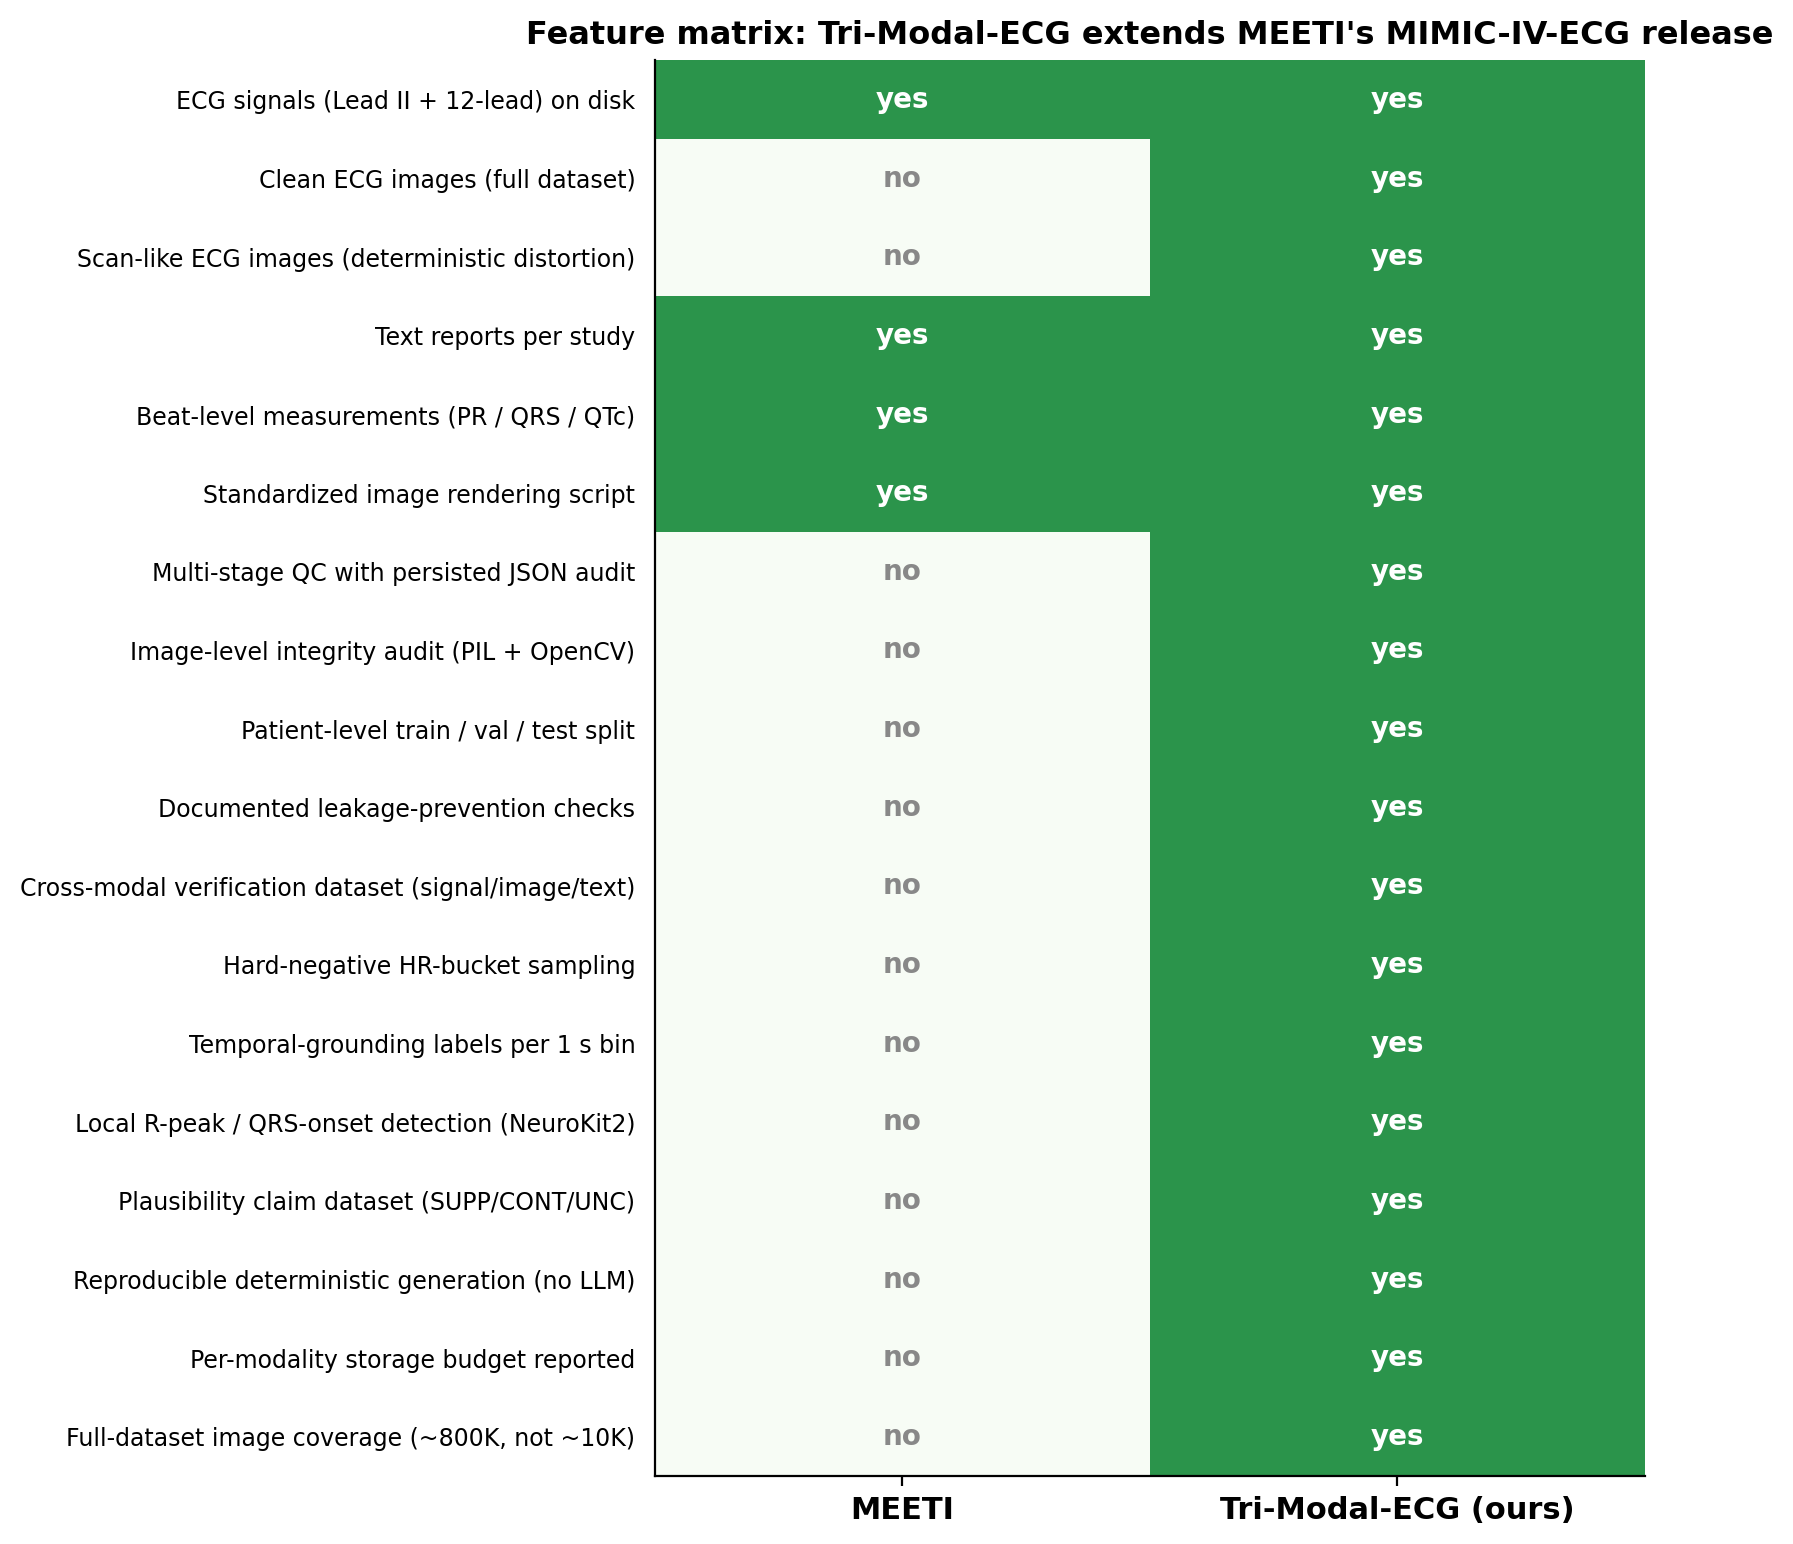
\includegraphics[width=0.92\linewidth]{fig_feature_matrix.png}
 \caption{Feature-level comparison of Tri-Modal-ECG and the MEETI release \cite{zhang2024meeti}. ``yes/no'' is decided from the released artefact: cells in the MEETI column reflect what is shipped in the MEETI repository (signals, $\sim$10{,}000 plotted images, beat-level features extracted by FeatureDB, MIMIC-IV report, GPT-4o interpretations); cells in our column reflect what is shipped in this release. Tri-Modal-ECG matches MEETI on the four core modalities and additionally provides full-coverage clean and scan-like images, a multi-stage persisted QC, patient-level splits with leakage checks, three deterministic benchmark tasks, and per-modality storage budgets.}
 \label{fig:feature_matrix}
\end{figure}

\begin{figure}[!ht]
 \centering
 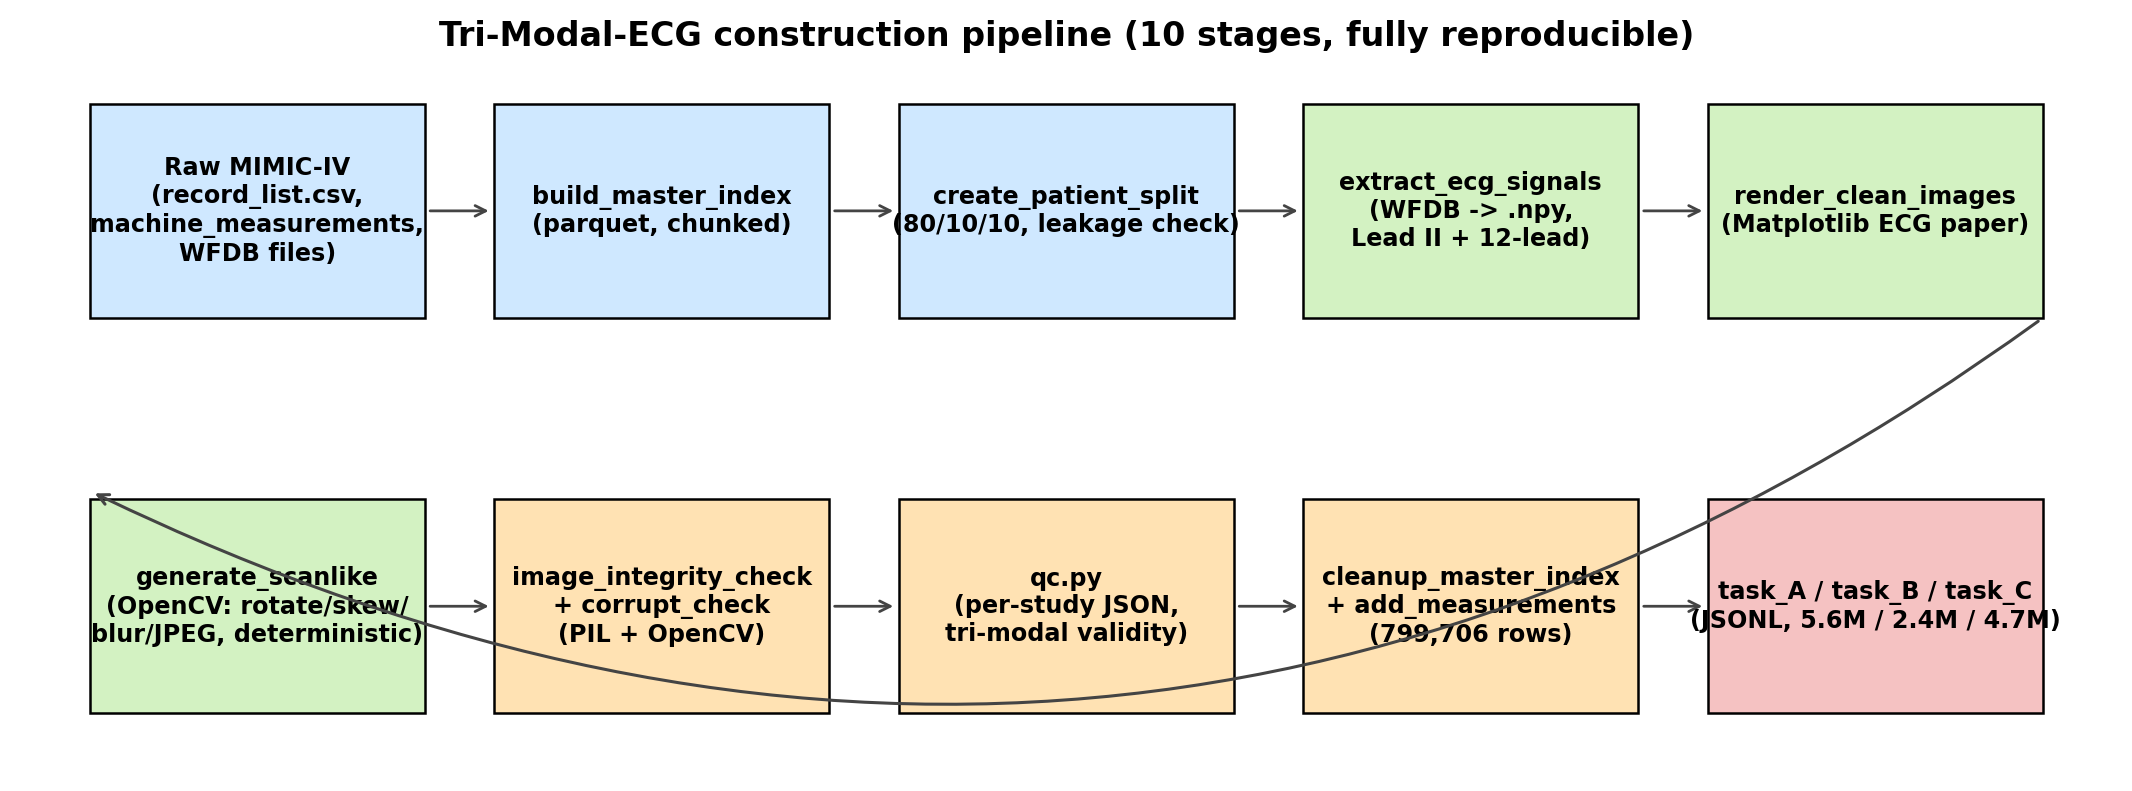
\includegraphics[width=\linewidth]{fig_pipeline_paper.png}
 \caption{Tri-Modal-ECG construction pipeline (10 stages). Blue boxes are indexing stages (master index from \texttt{record\_list.csv} and \texttt{machine\_measurements.csv}, patient-level split, leakage check). Green boxes are signal/image generation (WFDB \cite{xiao2018physionet} extraction to NumPy \cite{harris2020array}, Matplotlib \cite{hunter2007matplotlib} clean rendering, OpenCV \cite{bradski2000opencv} deterministic scan-like augmentation). Orange boxes are quality control (image integrity check using PIL+OpenCV decoders, per-study QC JSON, cleaned-index gating). Red box is the three benchmark tasks (verification / temporal grounding / plausibility) emitted as JSONL streams. Every stage is independently re-runnable from its on-disk inputs.}
 \label{fig:pipeline_paper}
\end{figure}

\section*{Methods}

\subsection*{Source data}

Tri-Modal-ECG is built directly on top of MIMIC-IV-ECG version 1.0 \cite{gow2023mimic, johnson2020mimic}, a publicly accessible diagnostic 12-lead ECG corpus drawn from routine clinical care at Beth Israel Deaconess Medical Center. From the upstream release we use three files: \texttt{record\_list.csv} ($800{,}035$ rows mapping \texttt{study\_id} to a WFDB record path), \texttt{machine\_measurements.csv} ($800{,}035$ rows of machine-generated text report fragments \texttt{report\_0}$\dots$\texttt{report\_17} and structured measurements (\texttt{rr\_interval}, \texttt{p\_onset}, \texttt{p\_end}, \texttt{qrs\_onset}, \texttt{qrs\_end}, \texttt{t\_end}, \texttt{p\_axis}, \texttt{qrs\_axis}, \texttt{t\_axis})), and the underlying WFDB waveform records under \texttt{data/files/}. Each waveform is 10{,}000-sample 12-lead but truncated to a uniform $5{,}000\times12$ matrix at $500$~Hz upon load with the WFDB-Python toolkit \cite{xiao2018physionet}; this corresponds to a standard 10-second diagnostic ECG.

\subsection*{Master index and patient-level split}

We build a master index by concatenating \texttt{report\_0}$\dots$\texttt{report\_17} into a single \texttt{T\_machine} text field per study, joined to the waveform path and \texttt{subject\_id}, and persisted as a single Apache Parquet file \cite{vaynberg2020apache}. Splits are constructed at the patient level: unique \texttt{subject\_id}s are shuffled with NumPy \cite{harris2020array} seed 42 and partitioned 80/10/10 into train, validation, and test subsets; every study inherits the split of its patient. We then verify that the three patient sets are pairwise disjoint, eliminating the dominant leakage mode for ECG datasets in which the same patient contributes multiple recordings (Figure~\ref{fig:ecgs_per_patient}, Table~\ref{tab:split}).

\begin{figure}[!ht]
 \centering
 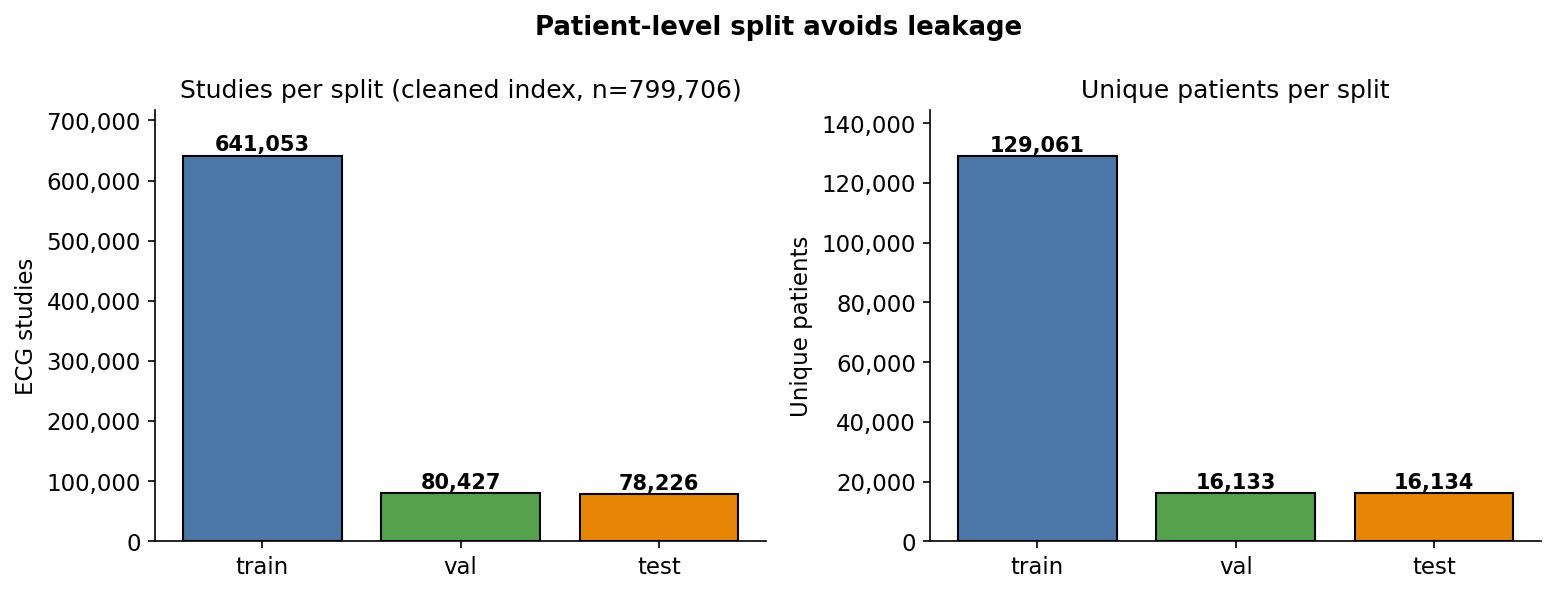
\includegraphics[width=0.95\linewidth]{fig_split_distribution.png}
 \caption{Studies and unique patients per split in the cleaned tri-modal dataset. The patient and study counts both follow the intended 80/10/10 ratio, and the construction script verifies $\text{train}\cap\text{val}=\text{train}\cap\text{test}=\text{val}\cap\text{test}=\emptyset$ at the patient level.}
 \label{fig:split}
\end{figure}

\begin{figure}[!ht]
 \centering
 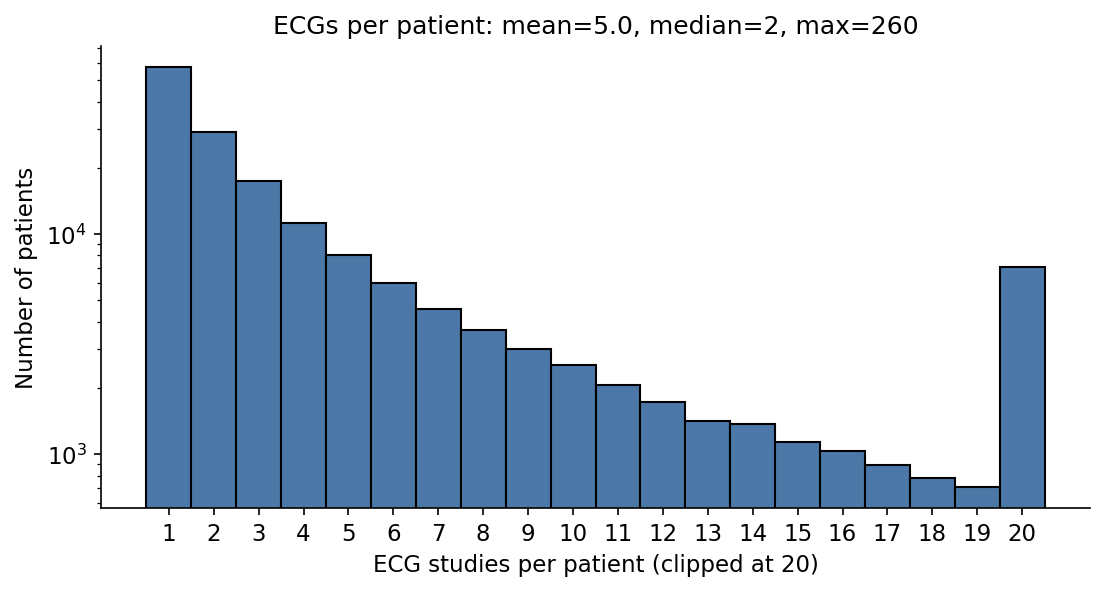
\includegraphics[width=0.7\linewidth]{fig_ecgs_per_patient.png}
 \caption{Distribution of ECGs per patient (cleaned dataset, log-scale $y$-axis, clipped at 20 ECGs per patient). The long tail---a small subset of patients contributes a disproportionate number of recordings---is the reason a study-level random split would massively contaminate validation and test, and motivates the patient-level partition described above.}
 \label{fig:ecgs_per_patient}
\end{figure}

\subsection*{Signal extraction}

For every study in the split index we read the WFDB record \cite{xiao2018physionet}, validate that all twelve leads are present, that Lead~II is one of them, and that the recording length is exactly $5{,}000$ samples, and persist three artefacts: \bpath{processed/signals_lead2/{study_id}.npy} (length-$5000$ float array), \bpath{processed/signals_12lead/{study_id}.npy} (shape-$(5000,12)$ float matrix), and \bpath{processed/signal_metadata/{study_id}.json} (lead names, sampling rate, file checksum). Lead~II is used by all downstream image and Task~B steps because it is the standard rhythm channel and is present in every diagnostic 12-lead ECG. Figure~\ref{fig:12lead} shows the raw 12-lead matrix for one cleaned study, exactly as it lands on disk; Figure~\ref{fig:lead2_conditions} shows Lead~II strips spanning the heart-rate and QRS-duration ranges in our dataset.

\begin{figure}[!ht]
 \centering
 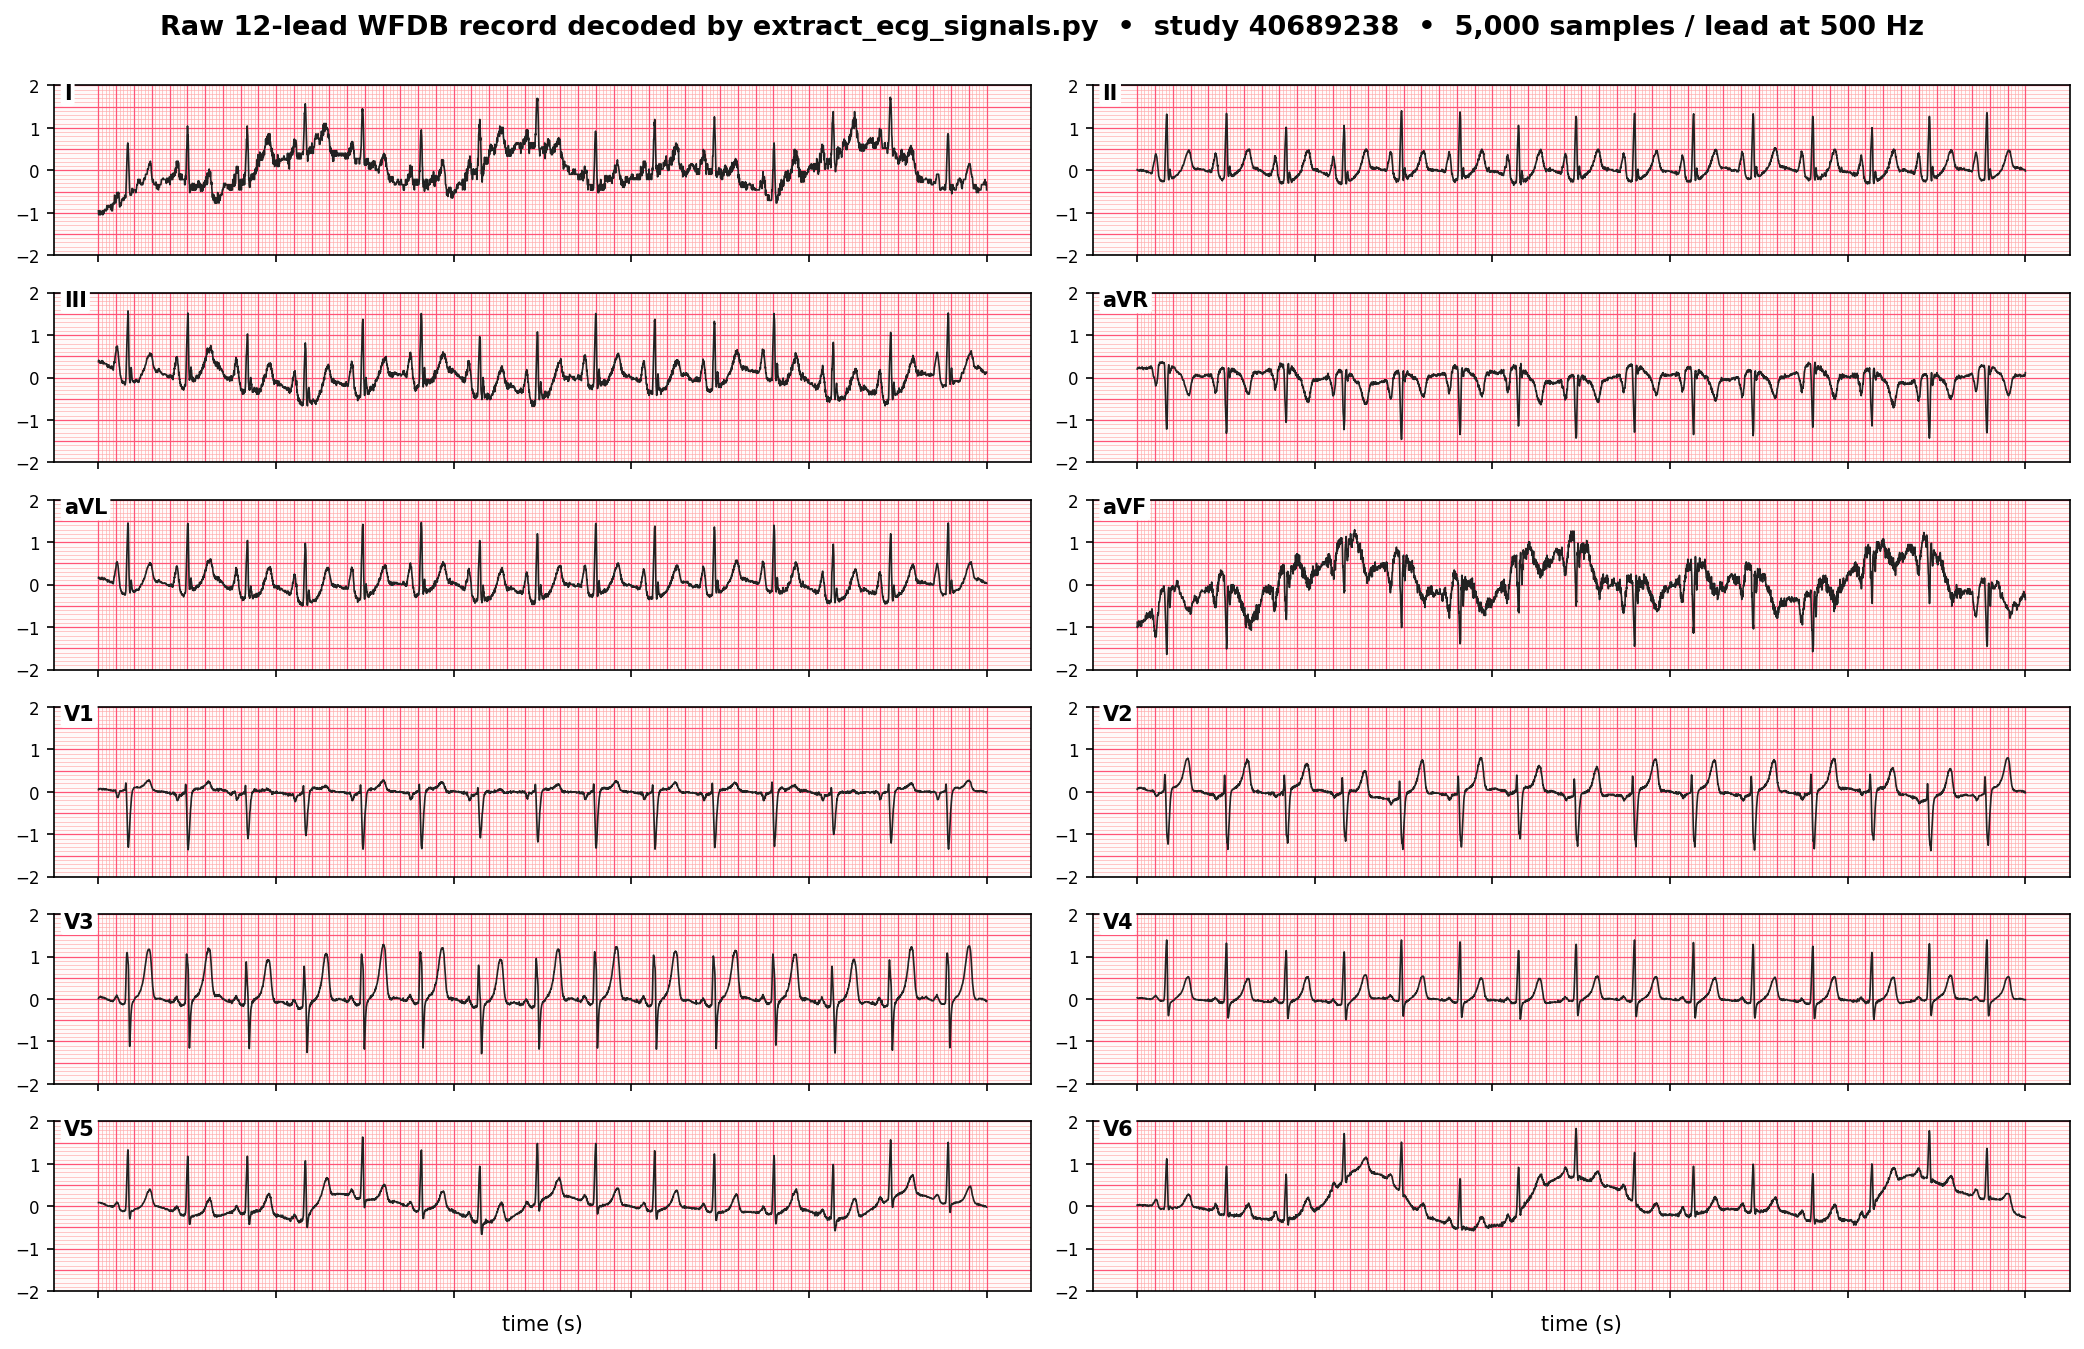
\includegraphics[width=\linewidth]{fig_12lead_montage.png}
 \caption{Raw 12-lead waveform matrix for a single cleaned study, exactly as stored in \texttt{signals\_12lead/\{study\_id\}.npy} (shape $5000\times12$, $500$~Hz). Lead~II (top right panel) is the rhythm strip used to render the clean ECG-paper image and to drive Task~B's local detection.}
 \label{fig:12lead}
\end{figure}

\begin{figure}[!ht]
 \centering
 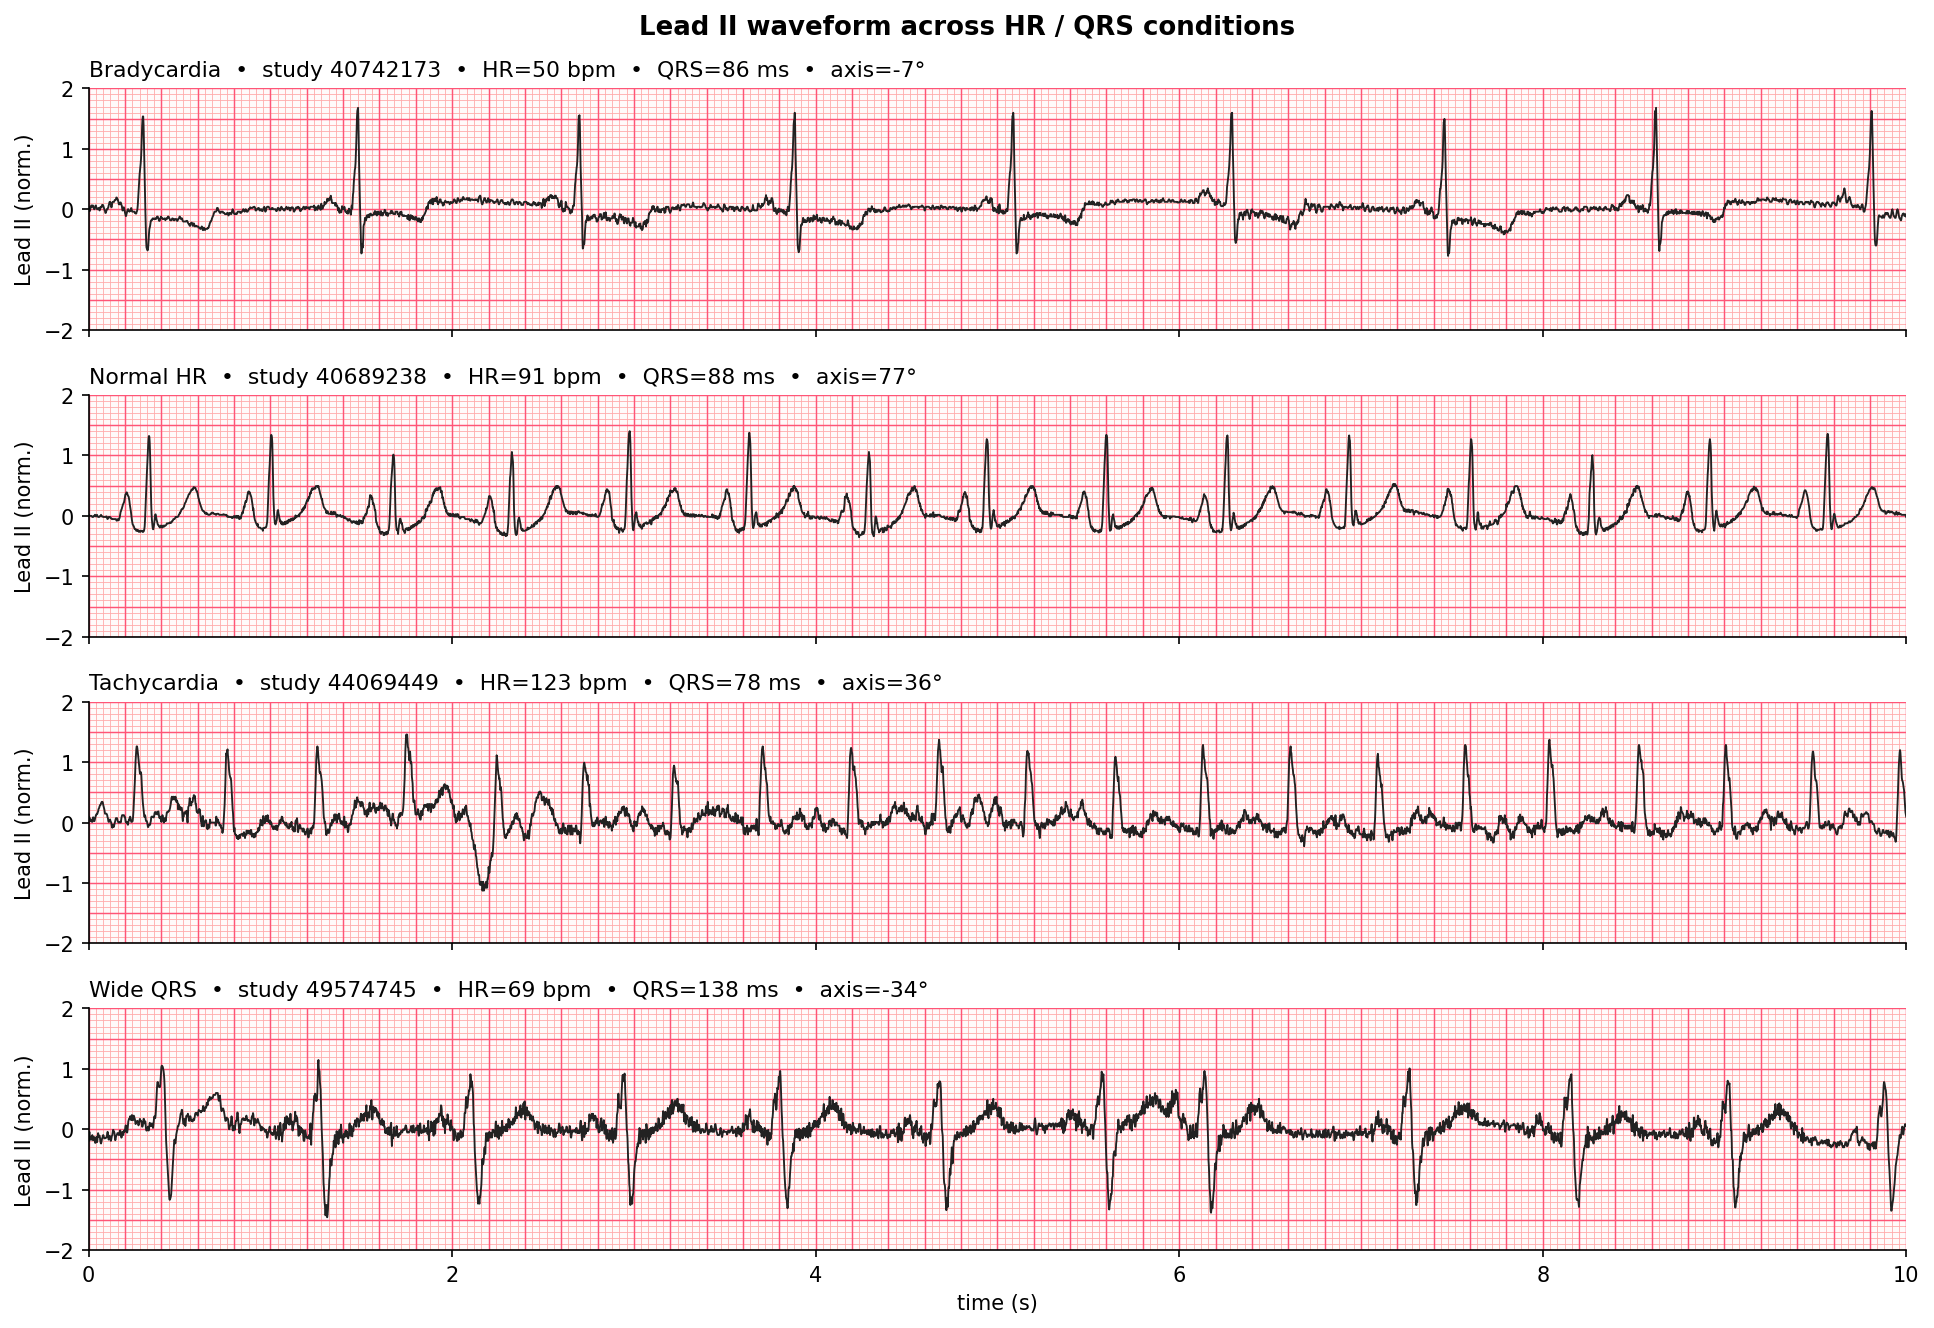
\includegraphics[width=\linewidth]{fig_lead2_conditions.png}
 \caption{Lead~II strips for four cleaned studies spanning the dataset's physiology range (bradycardia, normal rhythm, tachycardia, wide-QRS). All panels share the same time axis ($0$--$10$~s) and the same 99th-percentile amplitude normalization applied during clean-image rendering.}
 \label{fig:lead2_conditions}
\end{figure}

\subsection*{Clean ECG image rendering}

Each Lead~II array is rendered to a clean ECG-paper PNG with Matplotlib \cite{hunter2007matplotlib} using fixed parameters: figure size $12\times 2.5$~in, time axis $0$--$10$~s, $y$-range $[-2,2]$, light ECG-paper background colour \texttt{\#fffafa}, major $x$ grid every $0.2$~s and minor every $0.04$~s, major $y$ every $0.5$ and minor every $0.1$. Amplitude is normalised by dividing the signal by its 99th-percentile absolute amplitude and scaling by $1.2$, which clips outliers but preserves morphology (Figure~\ref{fig:normalization}). Studies for which the 99th-percentile amplitude is exactly zero (a flatline or fully saturated record) are detected, logged, and excluded rather than producing a meaningless image. Workers use Matplotlib's headless \texttt{Agg} backend; we leave two CPU cores free during rendering so the host system remains responsive.

\begin{figure}[!ht]
 \centering
 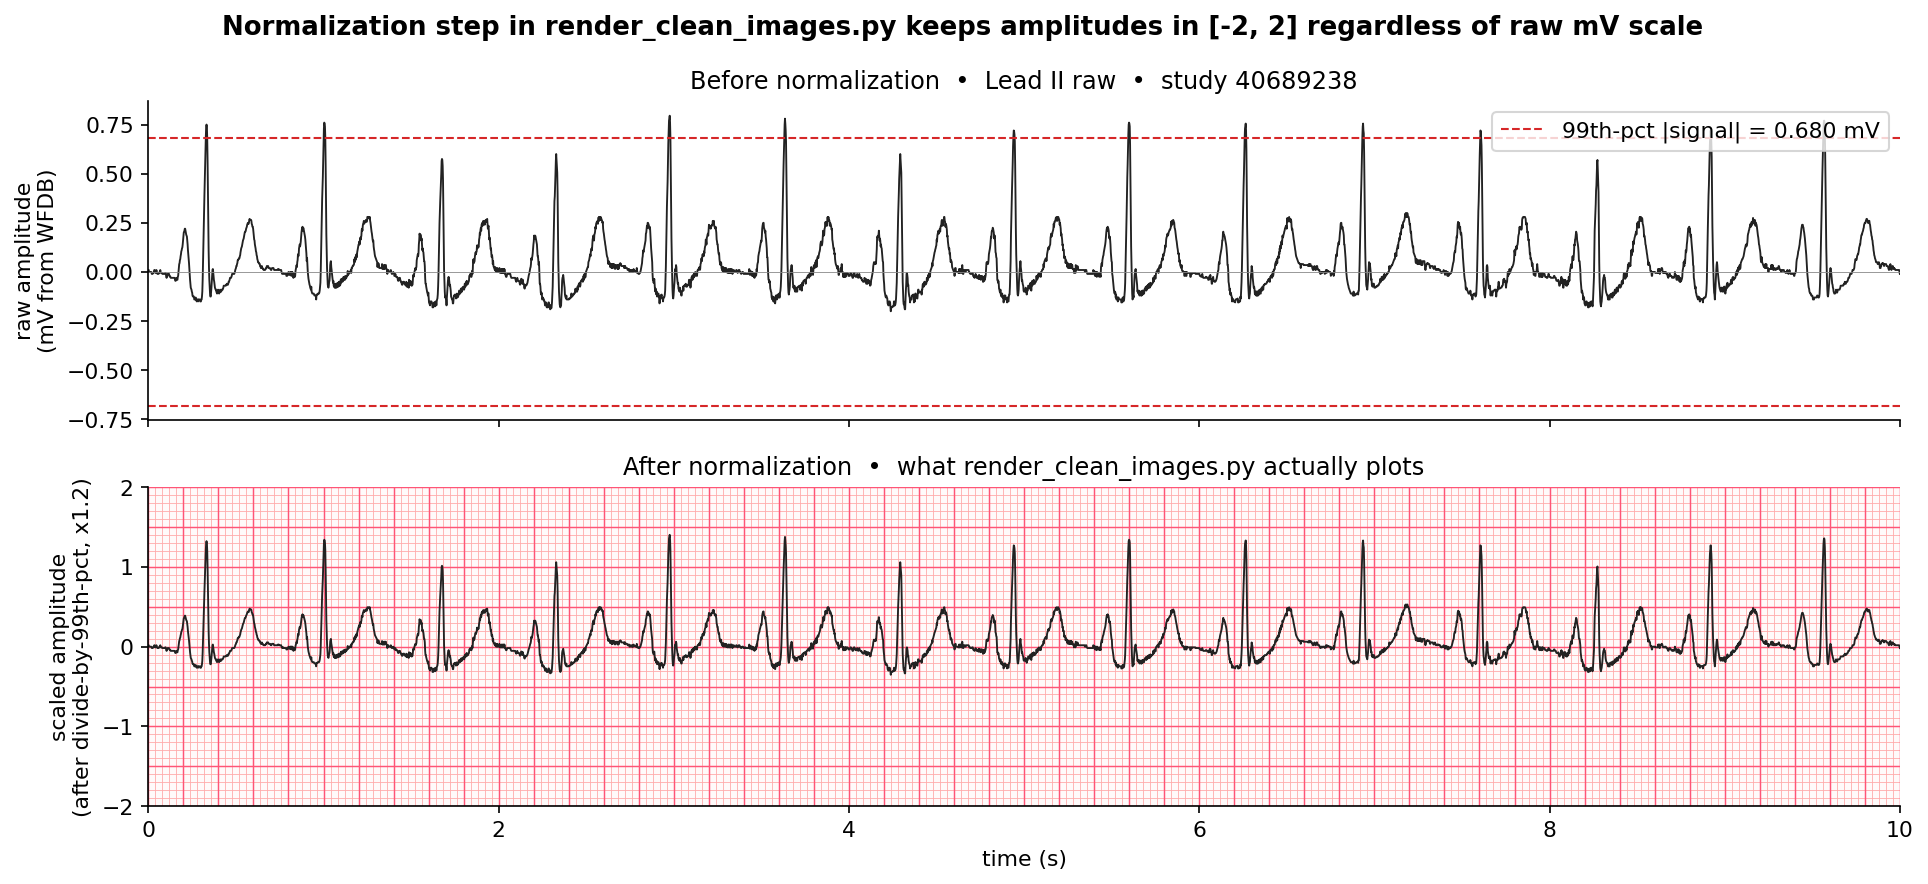
\includegraphics[width=0.8\linewidth]{fig_normalization.png}
 \caption{Effect of the 99th-percentile amplitude normalization (\texttt{render\_clean\_images.py}). Top: raw mV signal. Bottom: normalised signal that is actually drawn into the PNG. The normaliser is robust against single-sample artefacts but preserves the wave-by-wave morphology that downstream image models rely on.}
 \label{fig:normalization}
\end{figure}

\subsection*{Scan-like image generation}

Real-world ECG images often reach a model as scans or photos of paper, not as pixel-perfect plots. We therefore release a second image stream: a scan-like JPG produced from each clean PNG by a deterministic OpenCV \cite{bradski2000opencv} augmentation chain. For each study we (i) seed a NumPy generator from the integer \texttt{study\_id}, (ii) downscale the width to at most $1{,}600$ pixels, (iii) rotate by $\pm$2$^\circ$, (iv) apply a small perspective shift sampled in $[-1\%,+1\%]$ of width, (v) Gaussian-blur with kernel size $3$ or $5$, (vi) jitter brightness and contrast, and (vii) JPEG-encode with quality in $[70,95]$. Figure~\ref{fig:scanlike_pipeline} shows the six-step chain on one example, and Figure~\ref{fig:clean_vs_scan} shows clean / scan-like pairs across multiple physiological conditions. Because the seed depends on \texttt{study\_id} and not on a wallclock or worker index, the augmented JPG of a given record is bit-for-bit identical across rebuilds, which protects downstream evaluations against silent drift.

\begin{figure}[!ht]
 \centering
 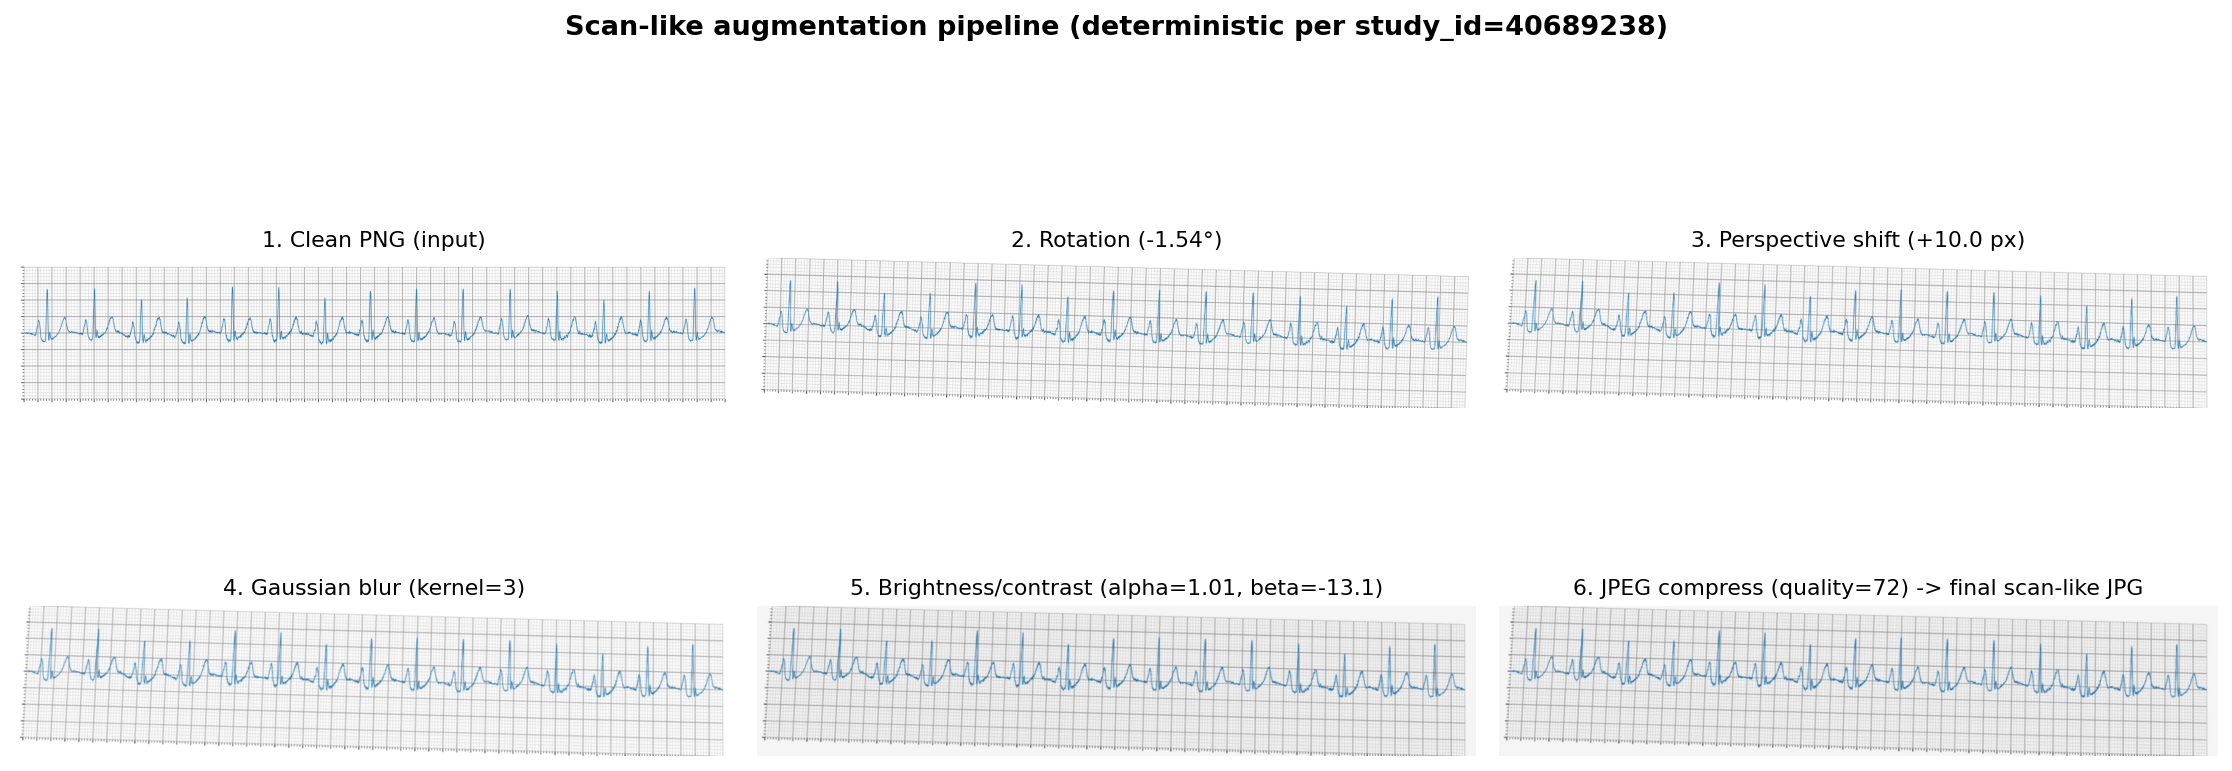
\includegraphics[width=\linewidth]{fig_scanlike_pipeline.png}
 \caption{Six-step deterministic scan-like augmentation chain applied to one clean PNG. The augmentation is seeded by \texttt{study\_id}; the rightmost panel matches the JPG that ends up on disk. The transform models the dominant degradations of real scanned clinical documents (mild rotation, perspective skew, optical blur, JPEG block artefacts) without altering the cardiac waveform.}
 \label{fig:scanlike_pipeline}
\end{figure}

\begin{figure}[!ht]
 \centering
 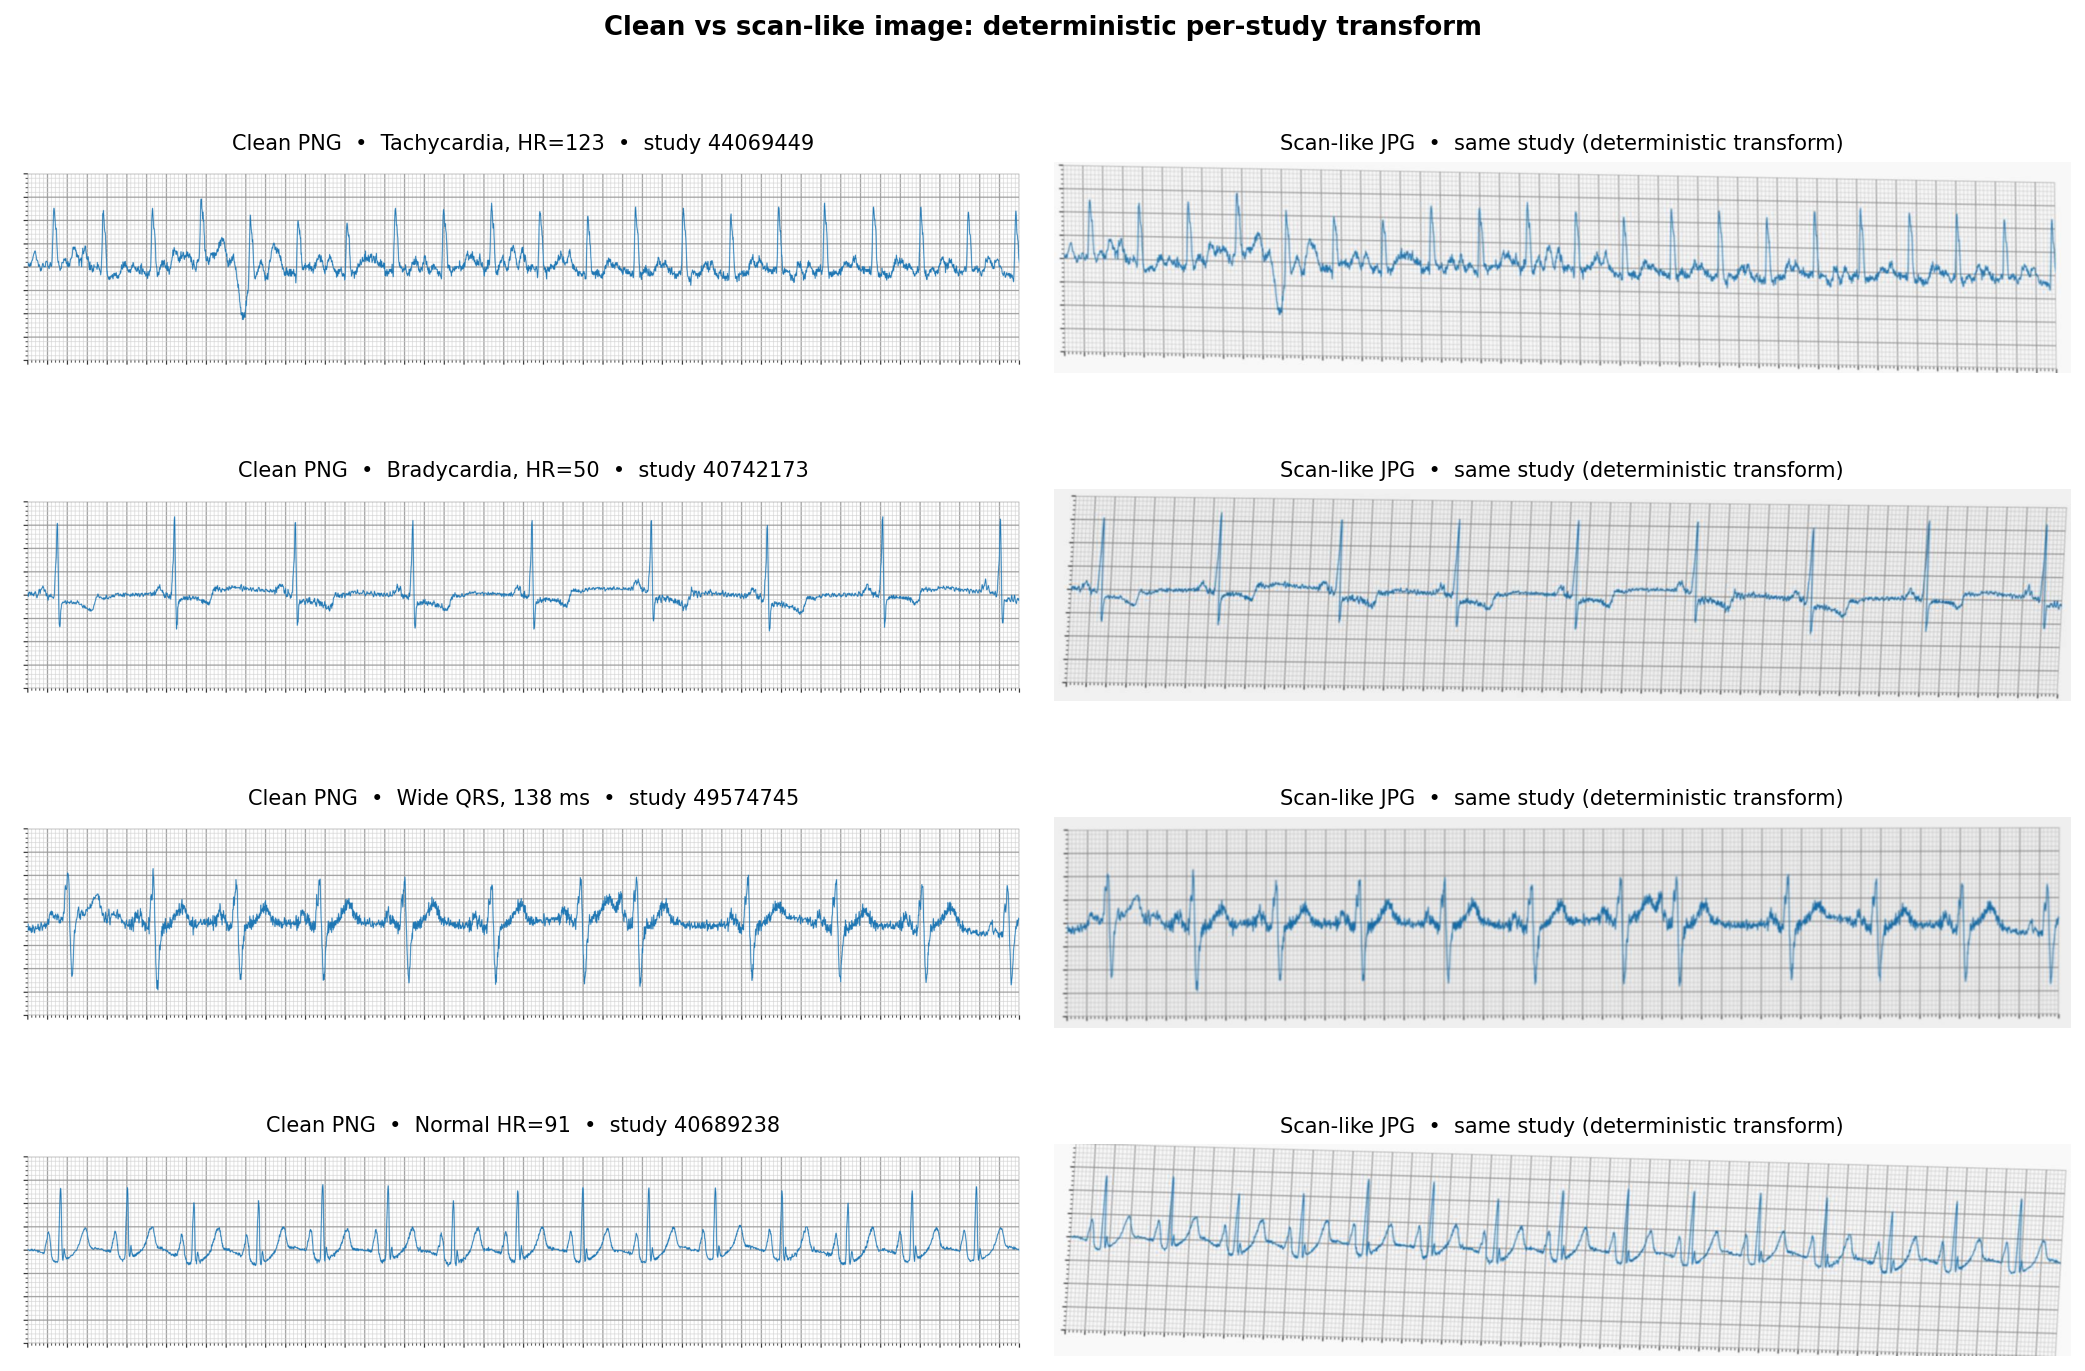
\includegraphics[width=\linewidth]{fig_clean_vs_scan.png}
 \caption{Clean PNG (left) and the matched scan-like JPG (right) for four cleaned studies spanning tachycardia, bradycardia, wide-QRS, and normal-HR rhythms. The deterministic transform preserves clinically relevant waveform features but reproduces realistic document degradation; both modalities are released for every study.}
 \label{fig:clean_vs_scan}
\end{figure}

\subsection*{Multi-stage quality control}

Quality control happens at four levels and is fully reproducible from on-disk artefacts. (1)~\emph{Image integrity audit}: each clean PNG is opened with both PIL (\texttt{img.verify()}) and OpenCV (\texttt{cv2.imread}) and required to have non-zero dimensions; each scan-like JPG is opened with OpenCV; missing files and decoder failures are written to per-modality regeneration lists. (2)~\emph{Regeneration loop}: missing or corrupt clean images are recomputed from their Lead~II \texttt{.npy} and scan-like images are re-derived from the resulting clean PNGs. (3)~\emph{Per-study tri-modal QC}: \texttt{qc.py} writes one JSON per study with \texttt{waveform\_ok} (Lead~II \texttt{.npy} loads and length is $5{,}000$), \texttt{image\_ok} (both clean and scan-like exist), and \texttt{text\_ok} (\texttt{T\_machine} non-empty); see Listing~\ref{lst:qcjson}. (4)~\emph{Cleaned-index gating}: \texttt{cleanup\_master\_index.py} keeps only studies with \texttt{waveform\_ok} $\wedge$ \texttt{image\_ok} $\wedge$ \texttt{text\_ok}, producing \texttt{index\_clean.parquet} ($799{,}706$ rows). Figure~\ref{fig:regeneration} shows the recovery effect of the regeneration loop: an intermediate run reported $173{,}784$ scan-like errors, after which the audit reports zero corrupt files and at most two missing files per modality. Figure~\ref{fig:qc_outcome} shows the final tri-modal QC pass/fail breakdown; Figure~\ref{fig:modality_coverage} shows per-modality file coverage.

\begin{lstlisting}[caption={Per-study QC JSON written by \texttt{qc.py}.},label={lst:qcjson},language=]
{
  "study_id": 40000017,
  "waveform_ok": true,
  "image_ok": true,
  "text_ok": true,
  "notes": ""
}
\end{lstlisting}

\begin{figure}[!ht]
 \centering
 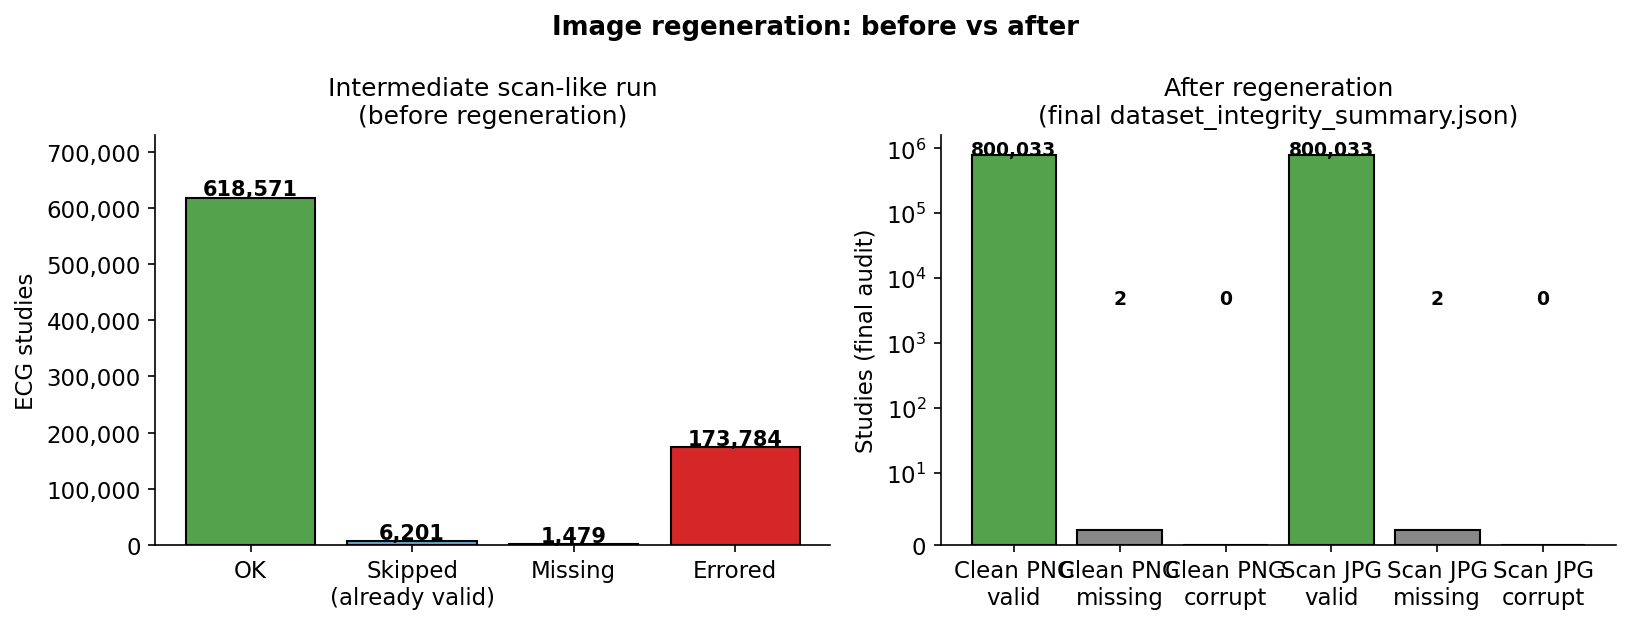
\includegraphics[width=0.95\linewidth]{fig_regeneration_before_after.png}
 \caption{Image regeneration loop, before (intermediate scan-like run) and after (final \texttt{dataset\_integrity\_summary.json}). The intermediate run reported 173{,}784 scan-like errors caused by transient I/O and decoder issues; iterative recomputation from the persisted Lead~II arrays reduced this to two missing scan-like images and zero corrupt scan-like images for the entire $800{,}035$-record table. The right panel uses a symmetric-log axis so the residual failures remain visible.}
 \label{fig:regeneration}
\end{figure}

\begin{figure}[!ht]
 \centering
 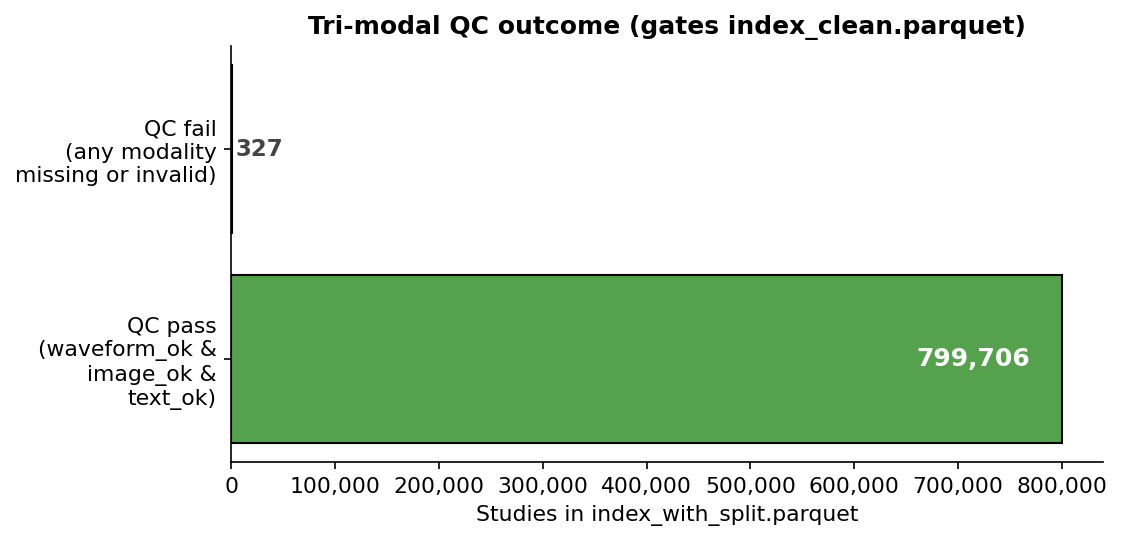
\includegraphics[width=0.7\linewidth]{fig_qc_outcome.png}
 \caption{Final tri-modal QC outcome on \texttt{index\_with\_split.parquet}: every study must pass the waveform, image and text checks to enter the cleaned index. $799{,}706$ of $800{,}033$ studies pass; the remaining $327$ are removed because at least one modality is missing or invalid. This gate is the single source of truth for which studies appear in any downstream task.}
 \label{fig:qc_outcome}
\end{figure}

\begin{figure}[!ht]
 \centering
 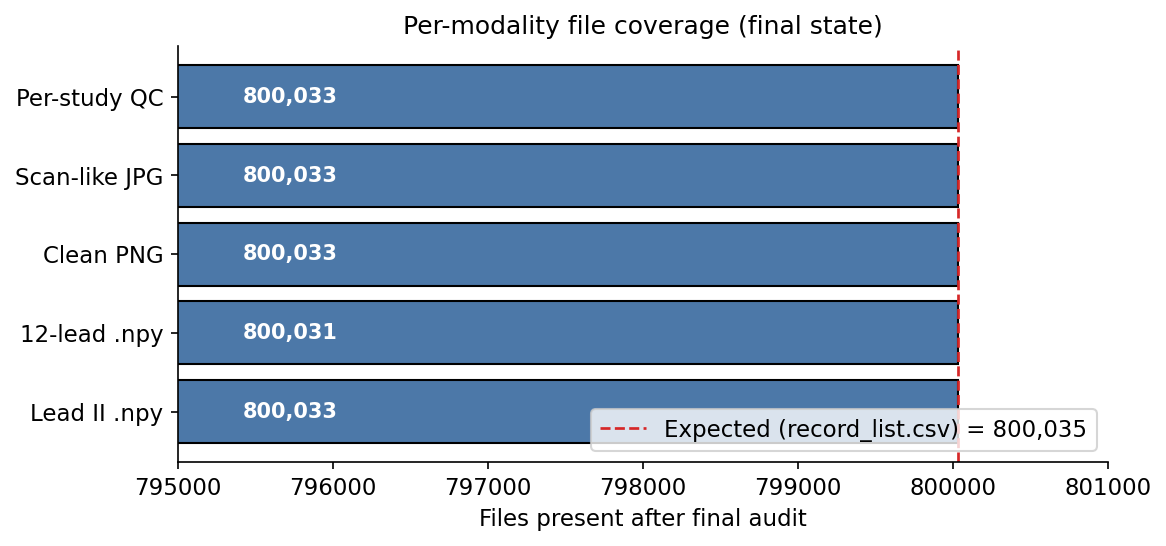
\includegraphics[width=0.7\linewidth]{fig_modality_coverage.png}
 \caption{Per-modality file coverage at the end of QC, plotted against the $800{,}035$ records expected from \texttt{record\_list.csv}. Lead~II arrays, 12-lead arrays, clean PNGs, and scan-like JPGs all reach within two files of the upper bound; per-study QC JSONs and signal metadata are produced for the smaller post-split index ($800{,}033$).}
 \label{fig:modality_coverage}
\end{figure}

\subsection*{Measurement enrichment}

After the cleaned index is produced, we merge nine structured fields from \bpath{machine_measurements.csv} (\texttt{rr\_interval}, \texttt{p\_onset}, \texttt{p\_end}, \texttt{qrs\_onset}, \texttt{qrs\_end}, \texttt{t\_end}, \texttt{p\_axis}, \texttt{qrs\_axis}, \texttt{t\_axis}) into the cleaned index, producing \bpath{index_clean_with_measurements.parquet}, the source of truth for Task~A and Task~C. To suppress the MIMIC-IV-ECG sentinel codes (\texttt{29999, 32767, 65535, $-32768$, $0$}) used to mark unavailable measurements we apply physiological-plausibility filters when reporting summary statistics in Section ``Technical Validation''; the underlying parquet retains the raw values so that other workflows can choose their own thresholds.

\section*{The three benchmark tasks}

\subsection*{Task A: cross-modal verification}

Task A asks: do this signal, this image, and this text belong to the same ECG study? For each cleaned study we emit two positive rows (\texttt{image\_type=clean} and \texttt{image\_type=scanlike}) and up to five negative rows: \texttt{TEXT\_SWAP}, \texttt{IMAGE\_SWAP}, \texttt{SIGNAL\_SWAP}, \texttt{PARTIAL\_MISMATCH} (image and text from another study, signal from anchor), and a same-heart-rate-bucket \texttt{HARD\_NEGATIVE\_TEXT} (text swapped from a study in the same HR bucket; only emitted if a same-bucket alternative exists). HR buckets are computed from \texttt{rr\_interval} as \texttt{brady} ($<60$ bpm), \texttt{normal\_low} ($60$--$80$), \texttt{normal\_high} ($80$--$100$), and \texttt{tachy} ($\geq 100$); see Figure~\ref{fig:hr_bucket_logic} for an end-to-end illustration of the same-bucket text swap. Figure~\ref{fig:taskA_negatives} walks through the full row-construction logic on a real anchor study, and Figure~\ref{fig:taskA_distribution} reports the final negative-type counts.

\begin{figure}[!ht]
 \centering
 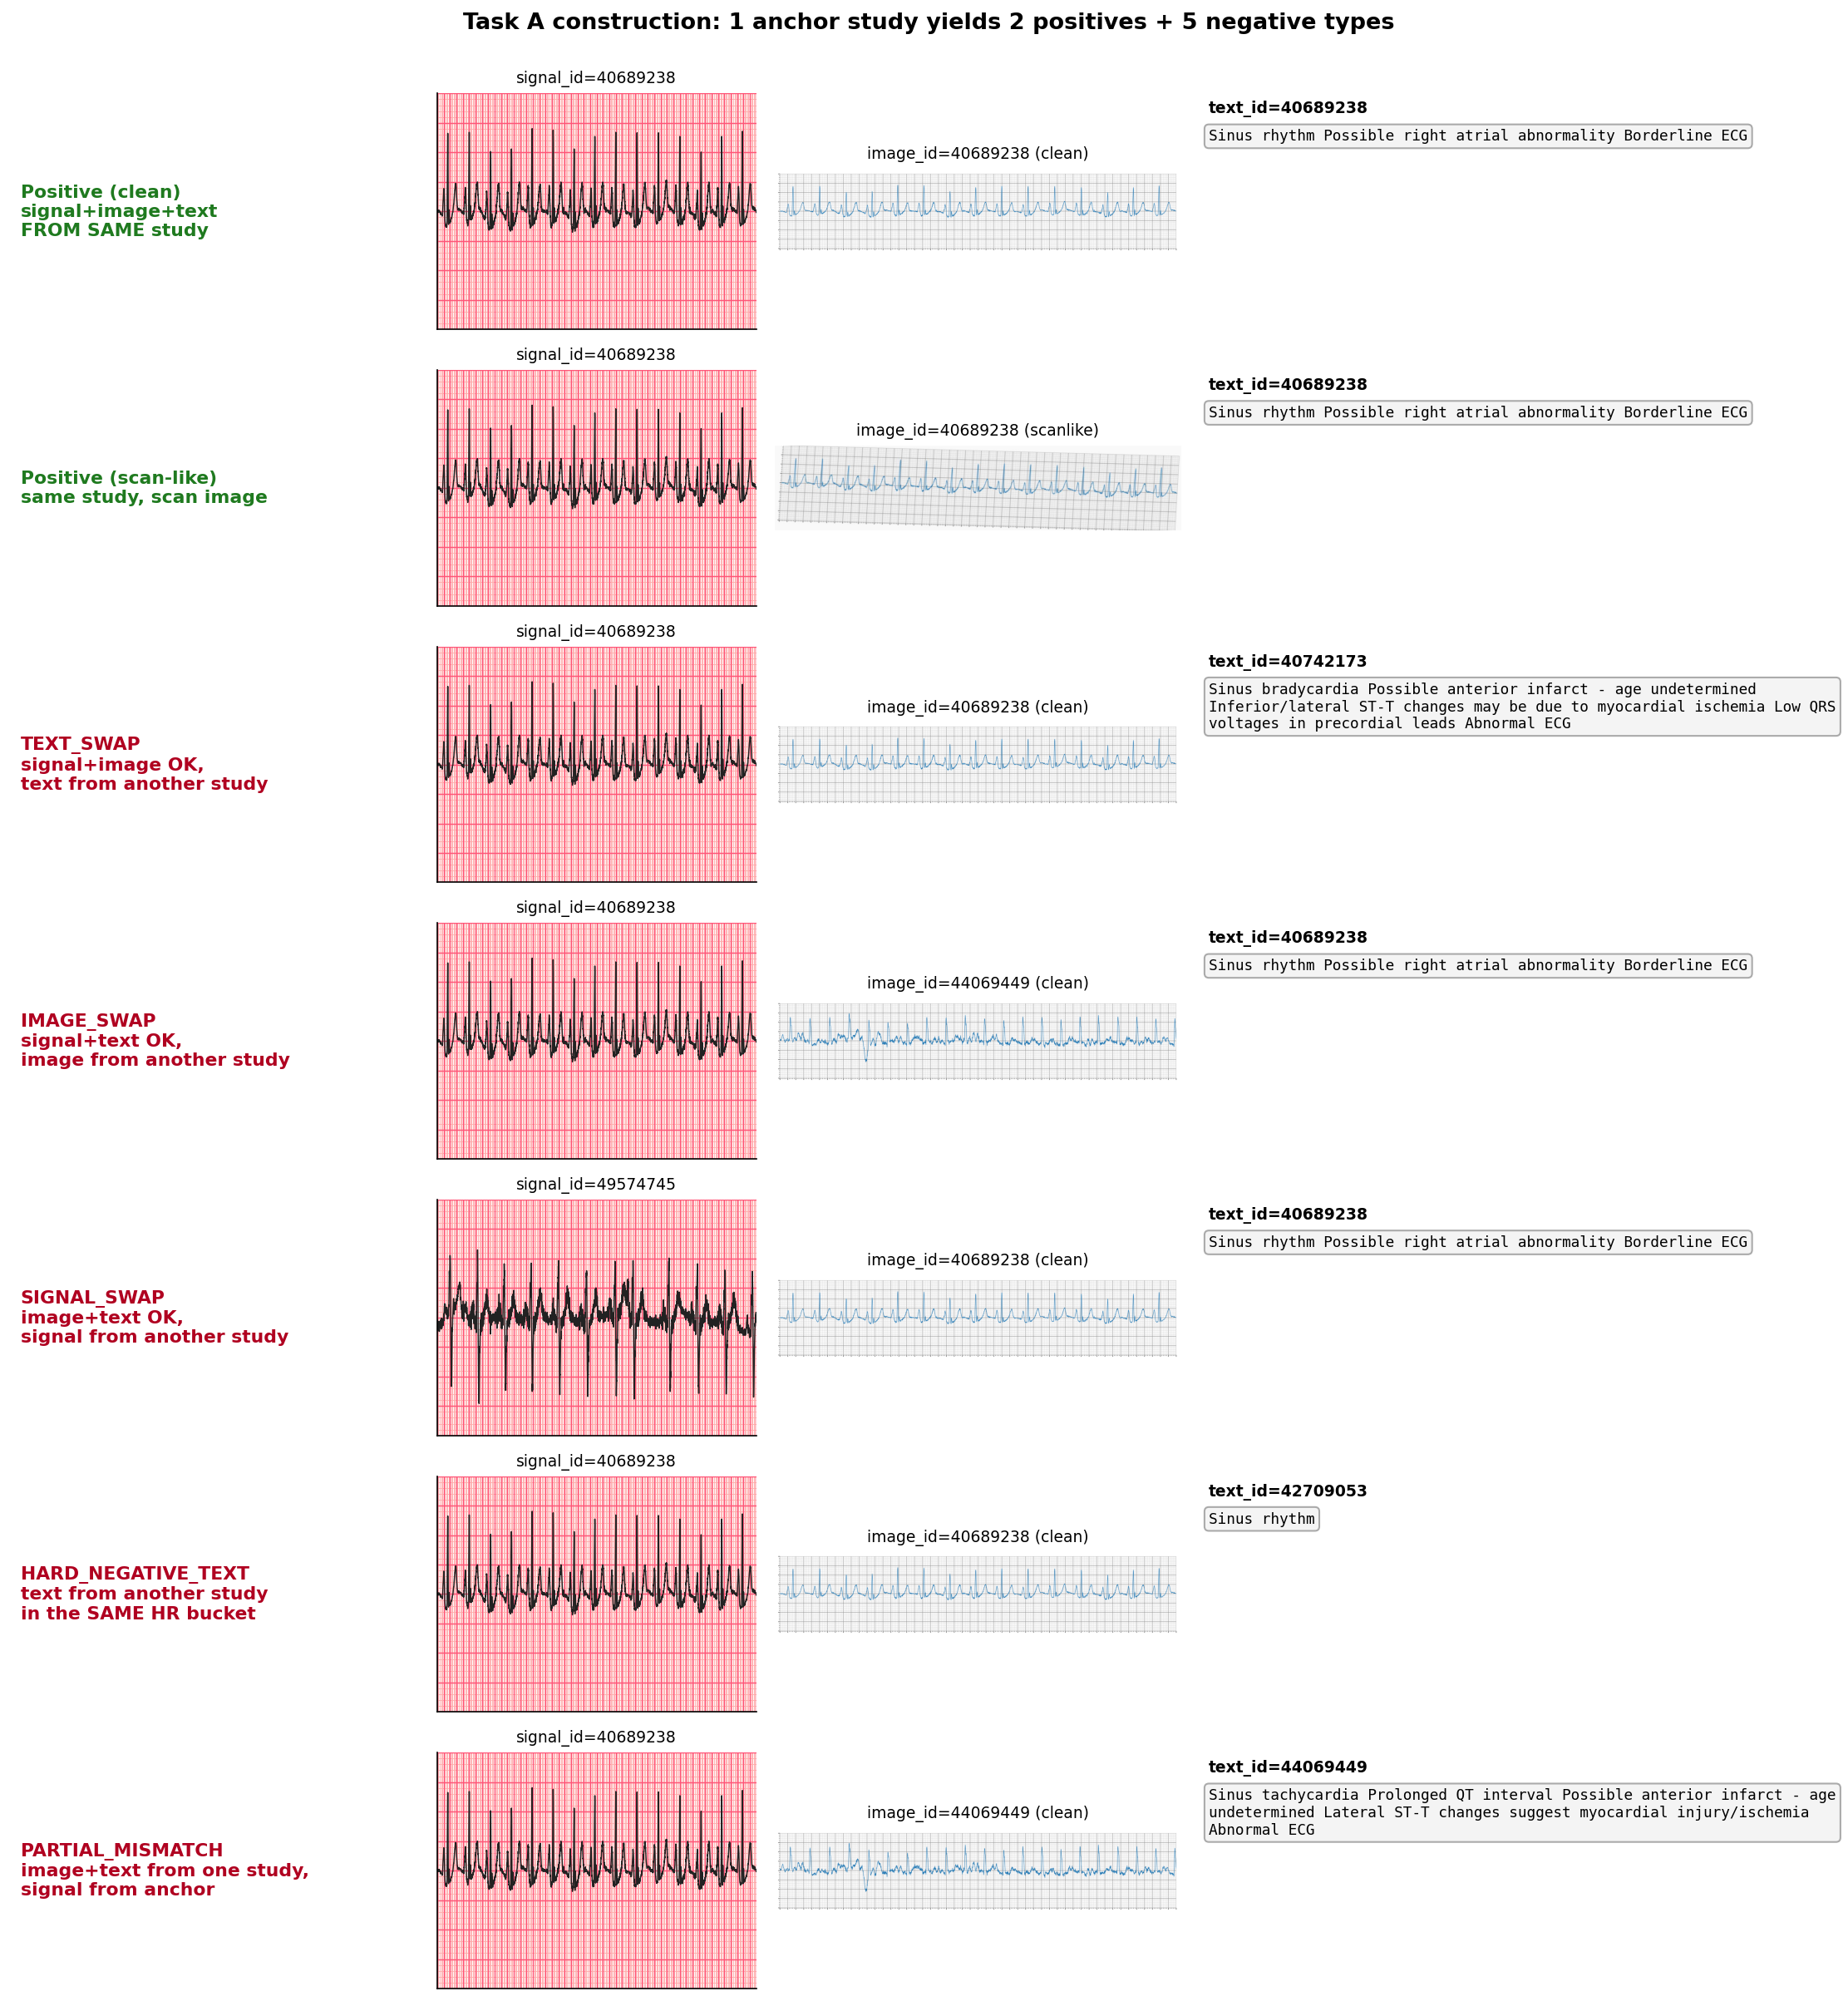
\includegraphics[width=\linewidth]{fig_taskA_negatives.png}
 \caption{Task~A row construction on a single anchor study. Green-titled rows are positives (clean and scan-like image, respectively). Red-titled rows are the five negative types. Each row's three columns show which study contributed the signal, the image, and the text; \texttt{TEXT\_SWAP} only changes the text source, \texttt{IMAGE\_SWAP} only changes the image source, etc. \texttt{HARD\_NEGATIVE\_TEXT} swaps text from a study in the same HR bucket, so heart-rate alone cannot solve the task.}
 \label{fig:taskA_negatives}
\end{figure}

\begin{figure}[!ht]
 \centering
 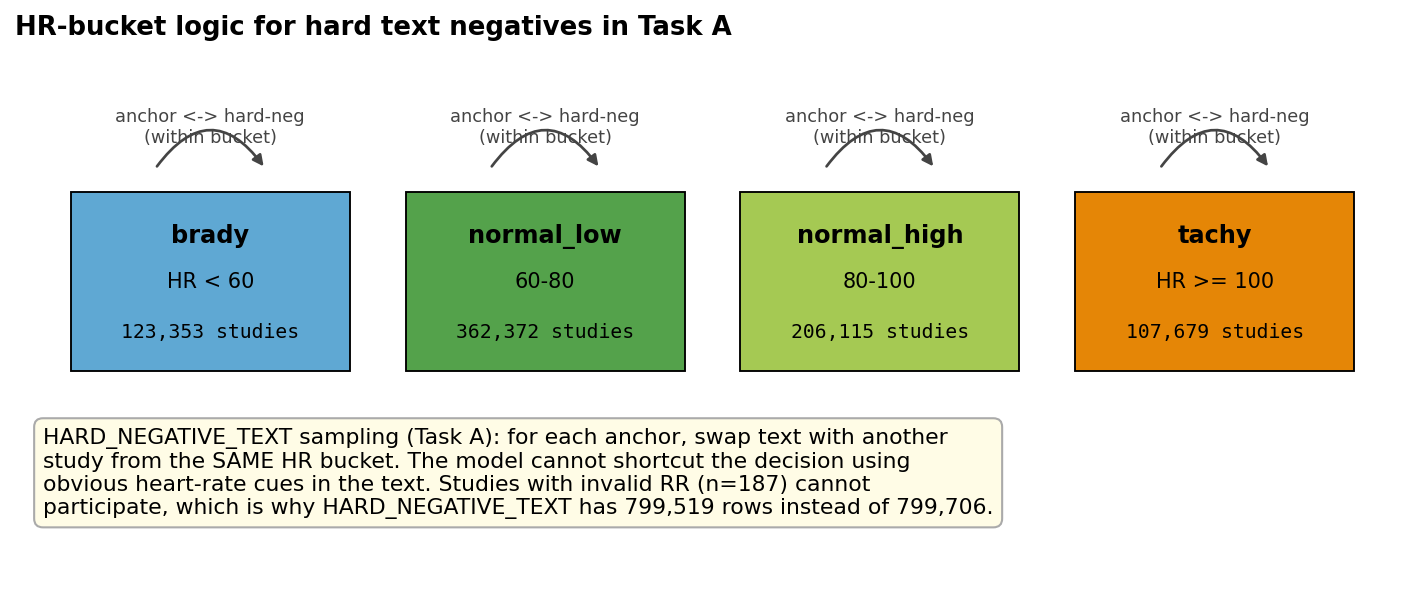
\includegraphics[width=\linewidth]{fig_hr_bucket_logic.png}
 \caption{Heart-rate buckets used to construct \texttt{HARD\_NEGATIVE\_TEXT} rows. Studies are partitioned into four buckets (\texttt{brady}, \texttt{normal\_low}, \texttt{normal\_high}, \texttt{tachy}) using the cut-points marked in Figure~\ref{fig:hr_distribution}; the hard-negative text is sampled from a study in the \emph{same} bucket as the anchor.}
 \label{fig:hr_bucket_logic}
\end{figure}

\begin{figure}[!ht]
 \centering
 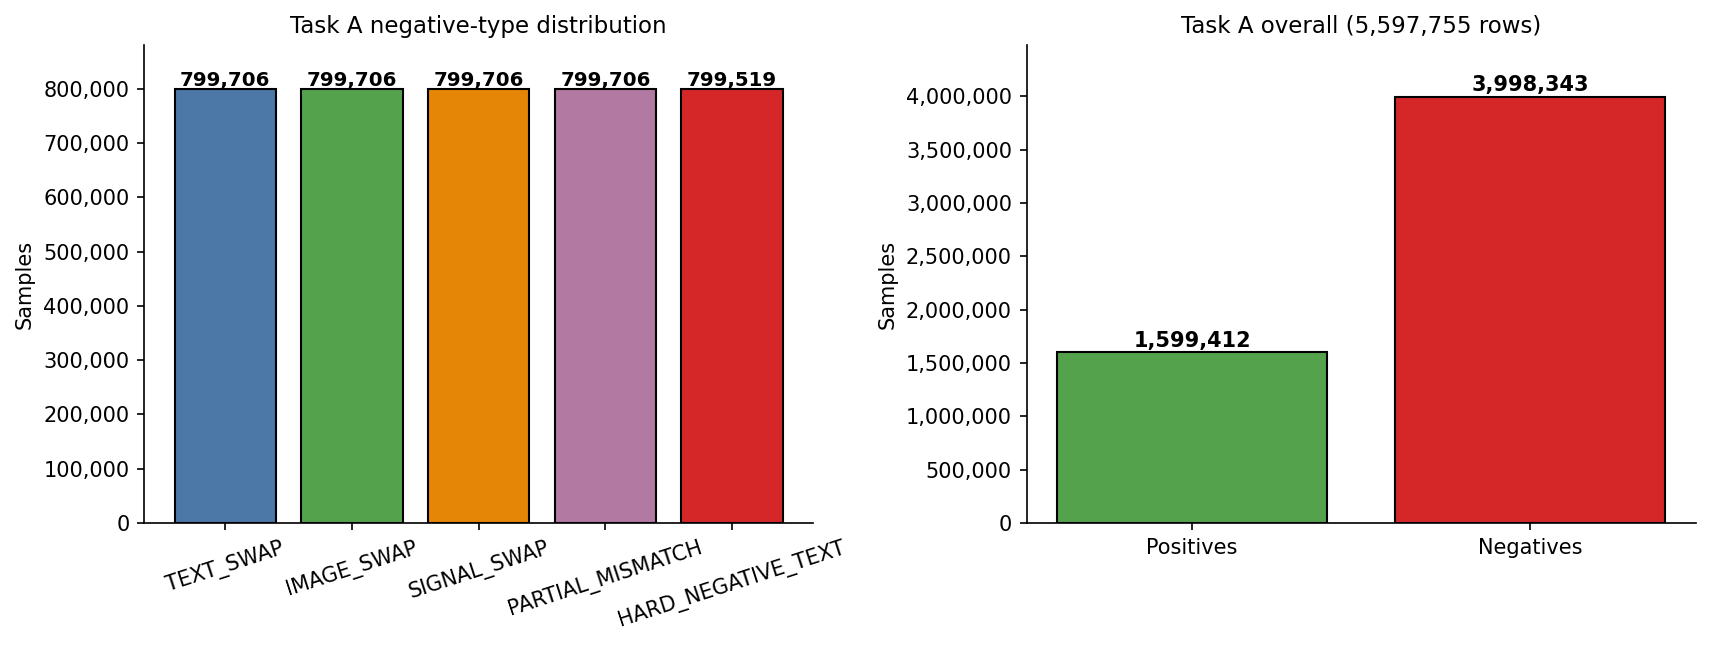
\includegraphics[width=\linewidth]{fig_taskA_distribution.png}
 \caption{Task~A negative-type and positive/negative distribution computed from \texttt{processed/taskA\_stats.json}. The five negative types are nearly equal in size because each is generated once per study; \texttt{HARD\_NEGATIVE\_TEXT} is the only exception, missing $187$ rows that correspond to the studies whose RR interval is invalid and therefore cannot be assigned a HR bucket.}
 \label{fig:taskA_distribution}
\end{figure}

\subsection*{Task B: temporal grounding (per-second labels via local detection)}

Task B associates a physiological query with the temporal regions of a 10-second ECG that satisfy it. Each study is divided into ten one-second bins (each bin is exactly $500$ samples at $500$~Hz) and we emit one row per (\texttt{study\_id}, \texttt{query}) pair carrying a length-10 binary label vector. The three queries are \texttt{HIGH\_HEART\_RATE} (local instantaneous HR $> 100$ bpm), \texttt{LOW\_HEART\_RATE} (local HR $< 60$ bpm), and \texttt{WIDE\_QRS} (a QRS complex with onset inside the bin whose duration exceeds $120$~ms).

\paragraph{Local detection logic.} An earlier baseline of Task~B used the global \texttt{rr\_interval} to set all ten bins to either $0$ or $1$, which carried no temporal signal. We replaced that logic with per-bin local detection backed by NeuroKit2 \cite{makowski2021neurokit2}. Specifically: (i) R-peak positions are detected on the full Lead~II signal with the Pan-Tompkins algorithm \cite{pan1985realtime} after a bandpass-filter clean (\texttt{nk.ecg\_clean}); (ii) we apply a start-of-signal artefact filter that drops the first detected R-peak when its first RR interval is both shorter than $50\%$ of the median of the remaining RR intervals \emph{and} shorter than $350$~ms (= 175 samples = $171$~bpm). This filter is necessary because Pan-Tompkins routinely emits a spurious peak in the first $\sim$300~ms of the recording due to filter ringing on the signal-onset transient; without the filter, $\sim$1--2\% of studies receive a false bin-0 label (an artificial $\sim$200~bpm first interval that contradicts the true rhythm); (iii) instantaneous HR is computed at the midpoint of each detected RR interval as $60\cdot \mathrm{FS}/\text{RR}_{\text{samples}}$ and per-bin HR is the mean of the midpoints inside that bin (with nearest-midpoint fallback for empty bins); (iv) QRS onsets and offsets are produced beat-by-beat by NeuroKit2's wavelet delineator (\texttt{ecg\_delineate}, method \texttt{dwt}) following the Mart\'{\i}nez et al.\ approach \cite{martinez2004wavelet}, and a bin is labelled $1$ if any beat with QRS onset inside that bin has duration $>60$ samples (=$120$~ms). When R-peak detection fails we fall back to the global \texttt{rr\_interval} rule for HR queries (and zeros for \texttt{WIDE\_QRS}, which cannot be inferred without QRS boundaries); the QC-cleaned index makes such fallbacks rare.

Figure~\ref{fig:taskB_local} contrasts the labels under the old and the new rule: under the old rule the per-bin positive fraction is identical across all ten bins for each query; under the new rule the per-bin fractions vary, demonstrating that the temporal localization signal in the labels is real. Figure~\ref{fig:taskB_examples} shows three real cleaned studies with mixed labels overlaid on the Lead~II strip---a \texttt{HIGH\_HEART\_RATE} bin only goes positive where the local instantaneous HR actually exceeds $100$~bpm. Table~\ref{tab:taskB_perbin} reports the exact per-bin positive count for each query, and Figure~\ref{fig:taskB_distribution} plots the per-query distribution.

\begin{figure}[!ht]
 \centering
 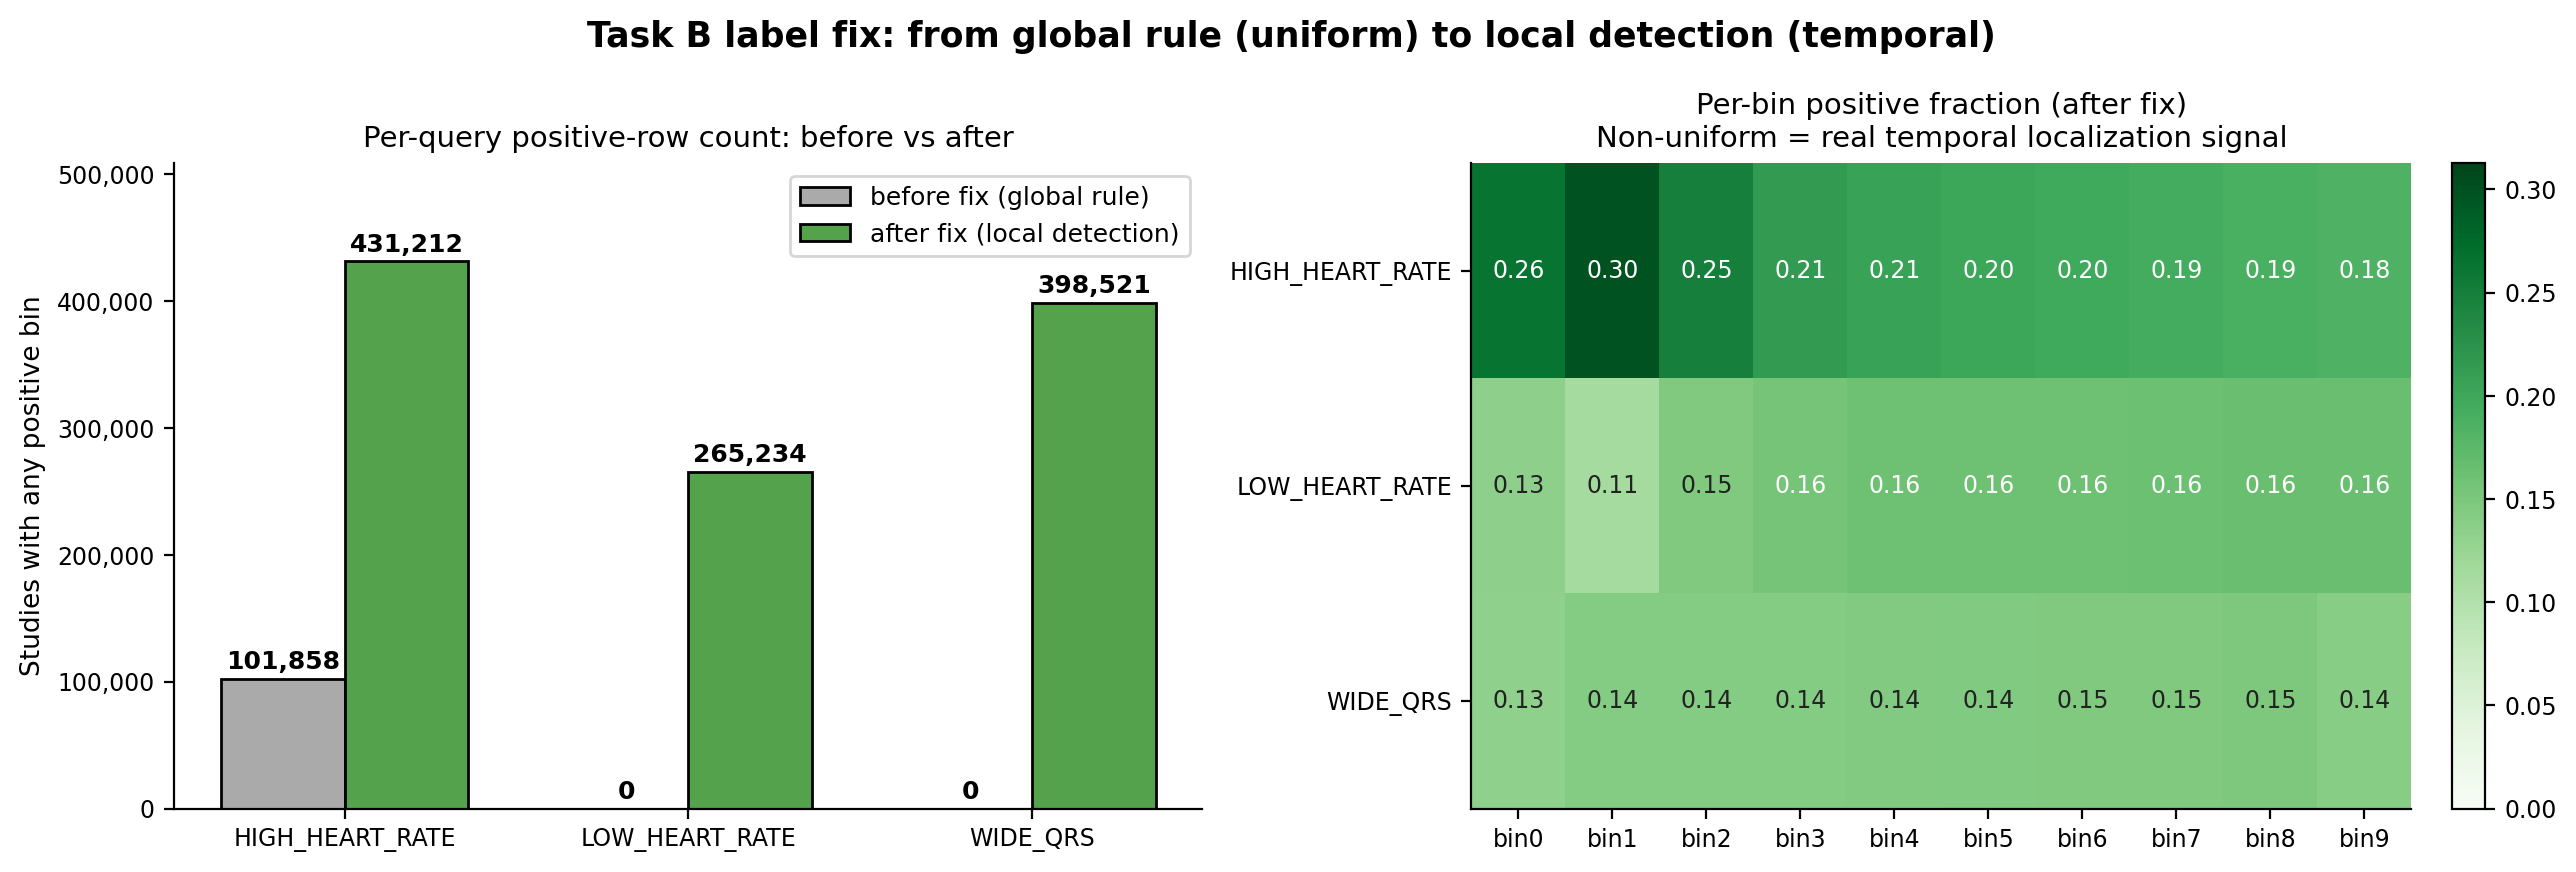
\includegraphics[width=\linewidth]{fig_taskB_before_after.png}
 \caption{Task~B label fix. Left: per-query count of studies with at least one positive bin, before vs after the fix. Under the old global-RR rule, \texttt{LOW\_HEART\_RATE} and \texttt{WIDE\_QRS} produced exactly zero positive rows because the rule only checked $\text{HR}>100$. After the fix, all three queries produce realistic positive counts that match the underlying physiology. Right: the post-fix per-bin positive fraction for the three queries; the non-uniform pattern across bins is the visual proof that local detection (rather than a global stamp) drives the labels.}
 \label{fig:taskB_local}
\end{figure}

\begin{figure}[!ht]
 \centering
 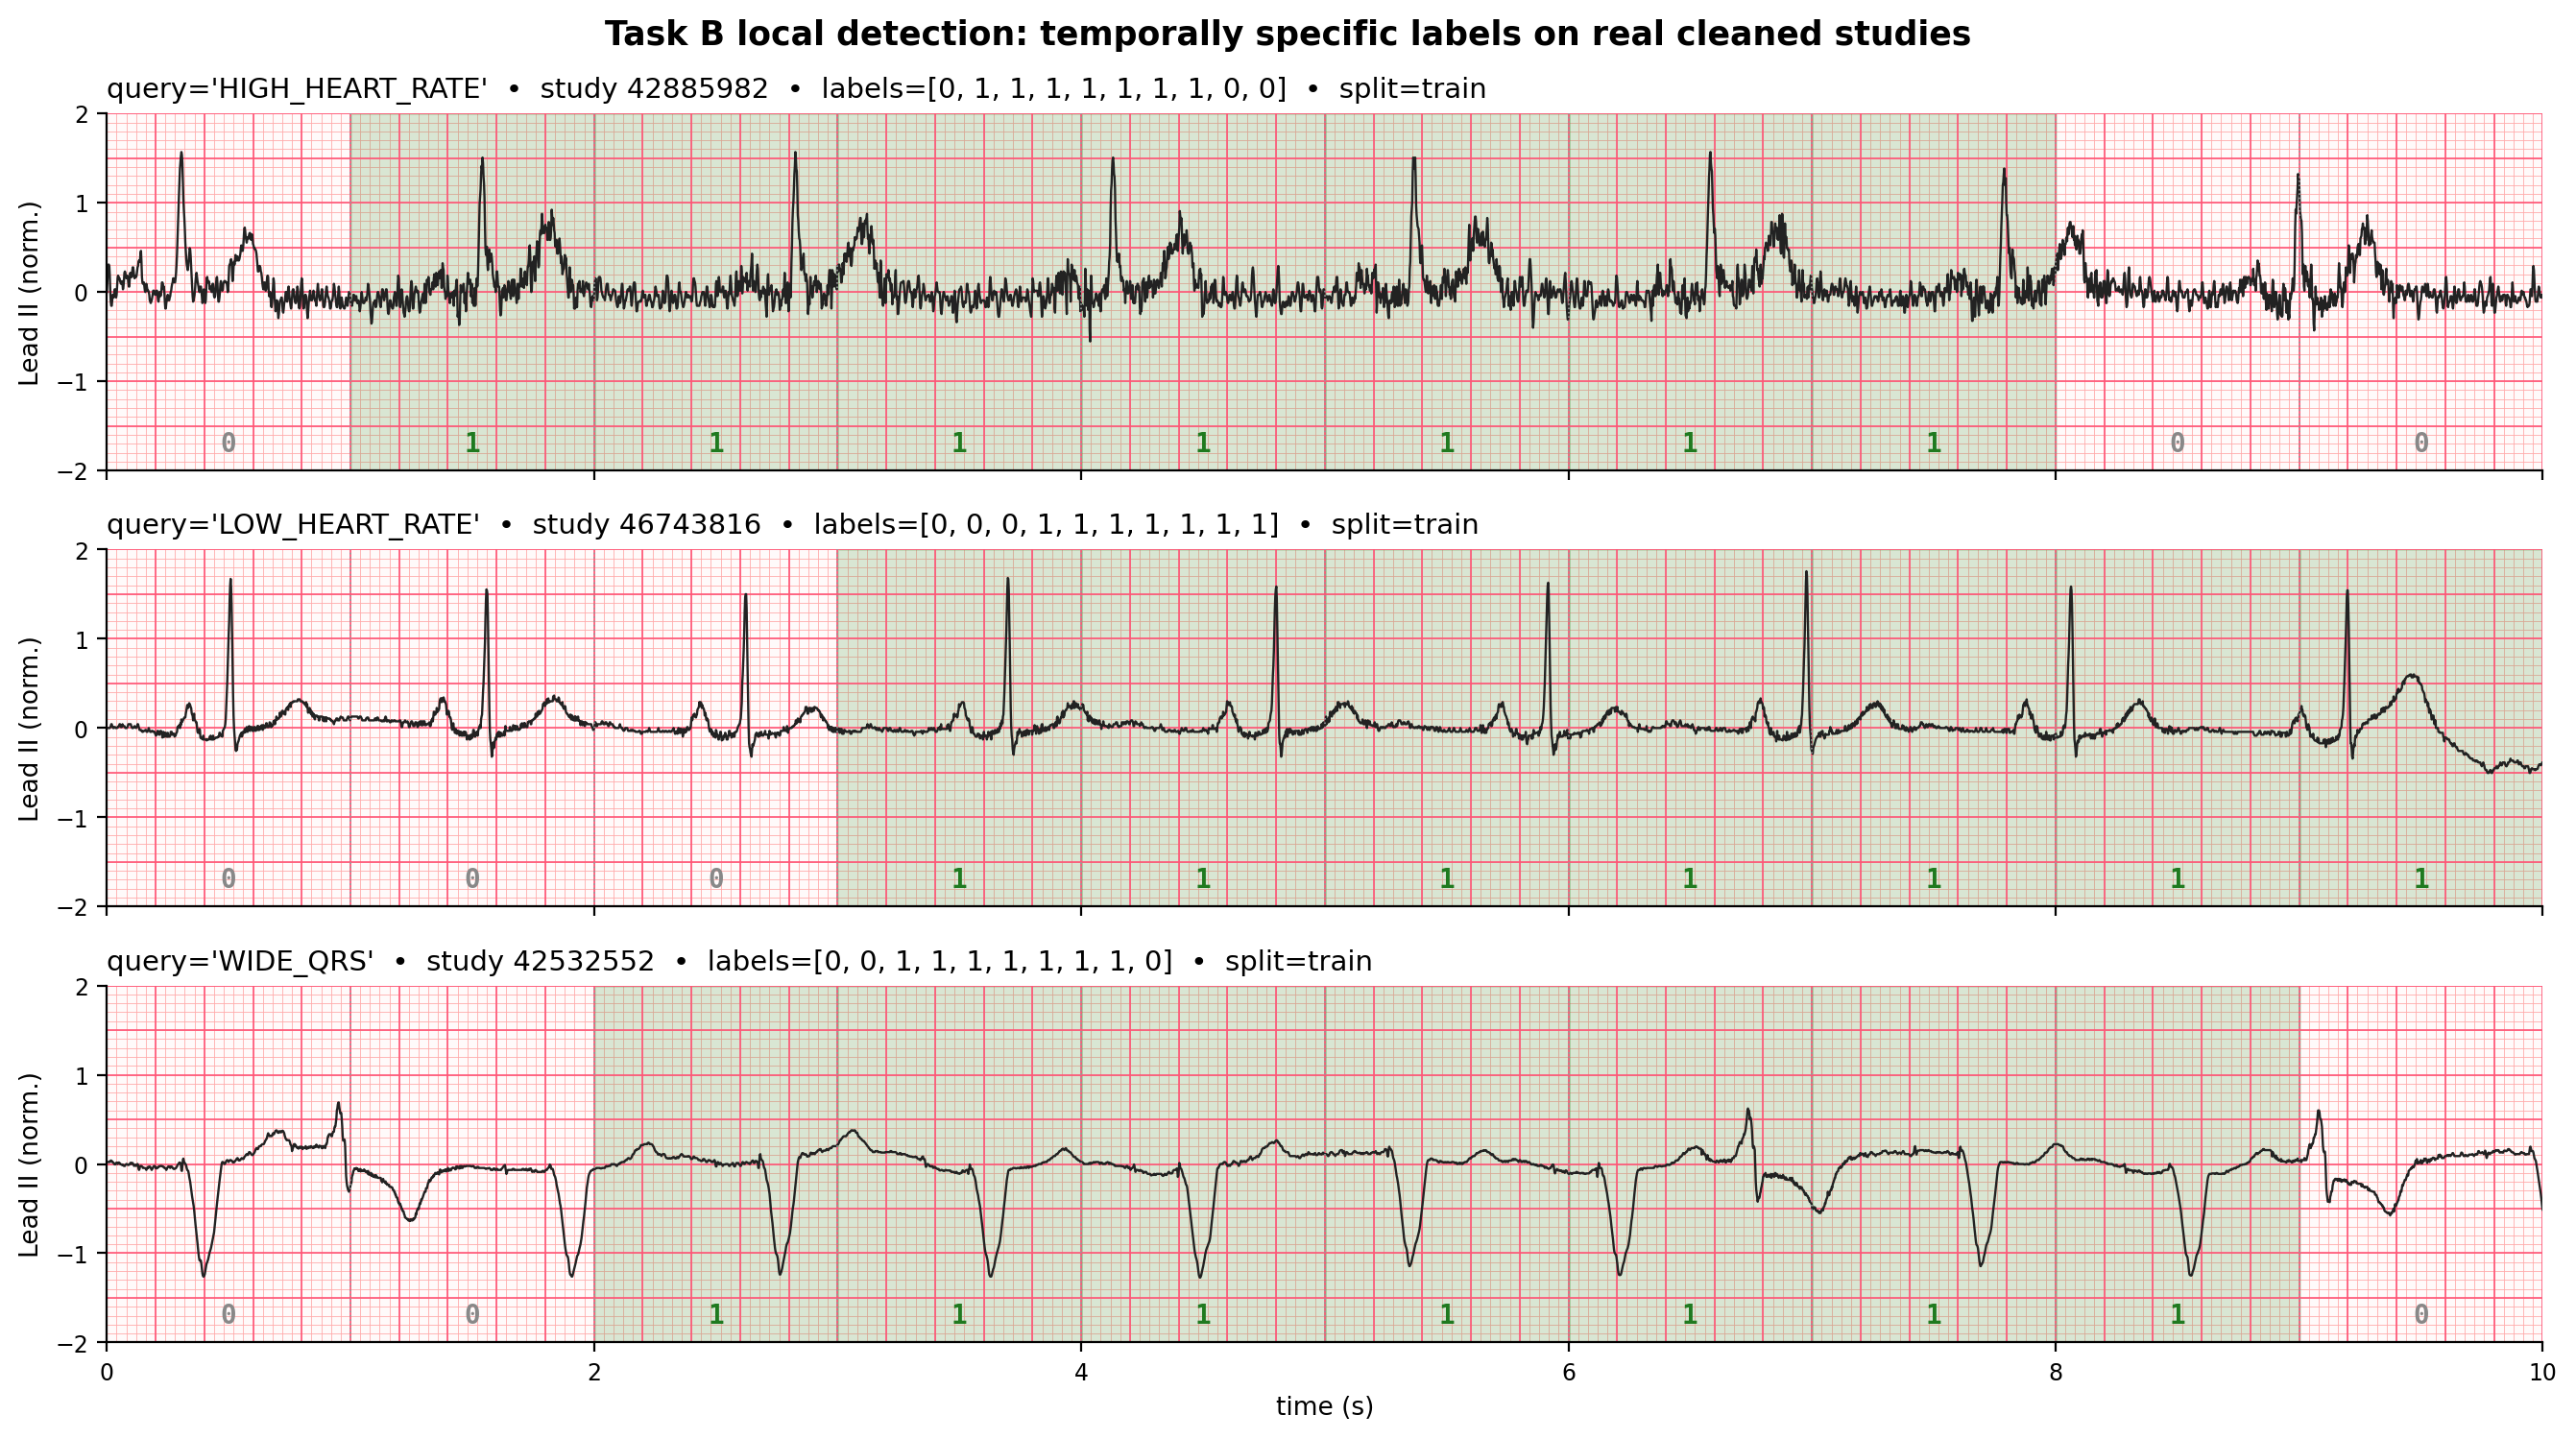
\includegraphics[width=\linewidth]{fig_taskB_examples.png}
 \caption{Task~B local detection on three real cleaned studies, one per query. Each panel overlays the per-bin label vector on the Lead~II waveform; bins labelled $1$ are shaded green. \textbf{Top:} \texttt{HIGH\_HEART\_RATE} study with a sustained tachycardic run --- bins 1--7 fire because the local instantaneous HR exceeds $100$~bpm there, while bins 0 and 8--9 stay $0$ where the rhythm is at or below the threshold. \textbf{Middle:} \texttt{LOW\_HEART\_RATE} study where the rate slows after roughly $3$~s and remains bradycardic for the rest of the strip, so bins 3--9 fire and the early bins stay $0$. \textbf{Bottom:} \texttt{WIDE\_QRS} study where wide-QRS beats appear from bin 2 through bin 8 (the wavelet delineator measures QRS duration $>120$~ms for those beats), and the very first and last bins do not fire because their beats either had borderline-narrow QRS or the delineator returned NaN boundaries. The old global rule would have collapsed each panel to all-zero or all-one; the per-bin patterns shown here are what makes the labels useful for temporal-grounding training.}
 \label{fig:taskB_examples}
\end{figure}

\begin{figure}[!ht]
 \centering
 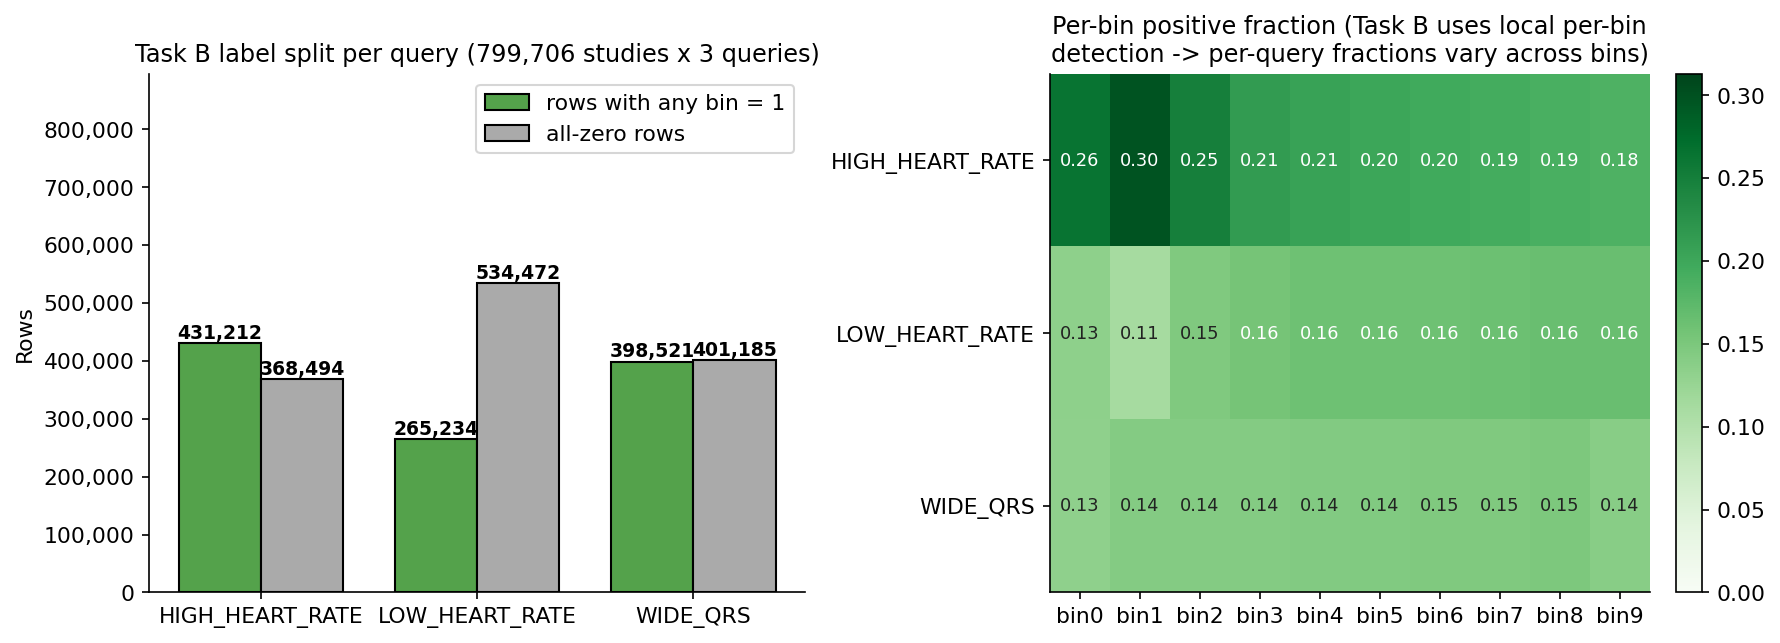
\includegraphics[width=\linewidth]{fig_taskB_distribution.png}
 \caption{Task~B per-query positive rate (left, fraction of studies with any positive bin) and per-bin positive fraction (right) computed by streaming the final \texttt{taskB\_temporal\_grounding.jsonl}. The per-bin fractions vary within each query, indicating real temporal information.}
 \label{fig:taskB_distribution}
\end{figure}

\begin{table}[!ht]
\centering
\caption{Task~B per-bin positive count per query (computed by streaming \texttt{taskB\_temporal\_grounding.jsonl}; total studies $=799{,}706$). The non-uniform within-query pattern across the ten bins is the quantitative counterpart of Figure~\ref{fig:taskB_local} and rules out the trivial all-bins-equal degenerate solution.}
\label{tab:taskB_perbin}
\renewcommand{\arraystretch}{1.15}
\resizebox{\textwidth}{!}{%
\begin{tabular}{l r r r r r r r r r r}
\toprule
Query & bin 0 & bin 1 & bin 2 & bin 3 & bin 4 & bin 5 & bin 6 & bin 7 & bin 8 & bin 9 \\
\midrule
\texttt{HIGH\_HEART\_RATE} & 210{,}266 & 238{,}254 & 198{,}553 & 171{,}331 & 164{,}817 & 161{,}081 & 156{,}830 & 153{,}509 & 151{,}130 & 147{,}643 \\
\texttt{LOW\_HEART\_RATE}  & 106{,}898 & 89{,}106 & 116{,}779 & 124{,}069 & 128{,}435 & 128{,}119 & 128{,}507 & 129{,}945 & 131{,}636 & 131{,}057 \\
\texttt{WIDE\_QRS}         & 105{,}904 & 113{,}366 & 113{,}933 & 113{,}917 & 114{,}615 & 115{,}530 & 116{,}503 & 117{,}265 & 118{,}486 & 111{,}269 \\
\bottomrule
\end{tabular}}
\end{table}

\subsection*{Task C: physiological plausibility}

Task C evaluates whether a short physiological text claim about a study is supported, contradicted, or undecidable given the study's structured measurements. We emit eight claims per study---\texttt{tachycardia present}, \texttt{bradycardia present}, \texttt{normal heart rate}, \texttt{wide qrs complex}, \texttt{normal qrs duration}, \texttt{left axis deviation}, \texttt{right axis deviation}, \texttt{axis normal}---paired with one of three labels: \texttt{SUPPORTED}, \texttt{CONTRADICTED}, or \texttt{UNCERTAIN} (only if the underlying measurement is missing or invalid). The decision rules are deterministic: HR is computed from \texttt{rr\_interval} as $60{,}000/\text{rr}$, QRS duration from $\text{qrs\_end}-\text{qrs\_onset}$, and axis from \texttt{qrs\_axis} (left $<-30^\circ$, right $>+90^\circ$, normal otherwise). Where possible, a single measurement emits two rows---a \texttt{SUPPORTED} row for the matching claim and a \texttt{CONTRADICTED} row for its inverse---which preserves the natural physiological distribution while balancing both label classes (Figure~\ref{fig:taskC_walkthrough}). The result is a $4{,}726{,}480$-row corpus where SUPPORTED and CONTRADICTED are nearly balanced (Figure~\ref{fig:taskC_distribution}, Figure~\ref{fig:taskC_heatmap}), and where UNCERTAIN appears only on heart-rate claims for the $187$ studies with invalid RR (374 rows after both heart-rate claims fire).

\begin{figure}[!ht]
 \centering
 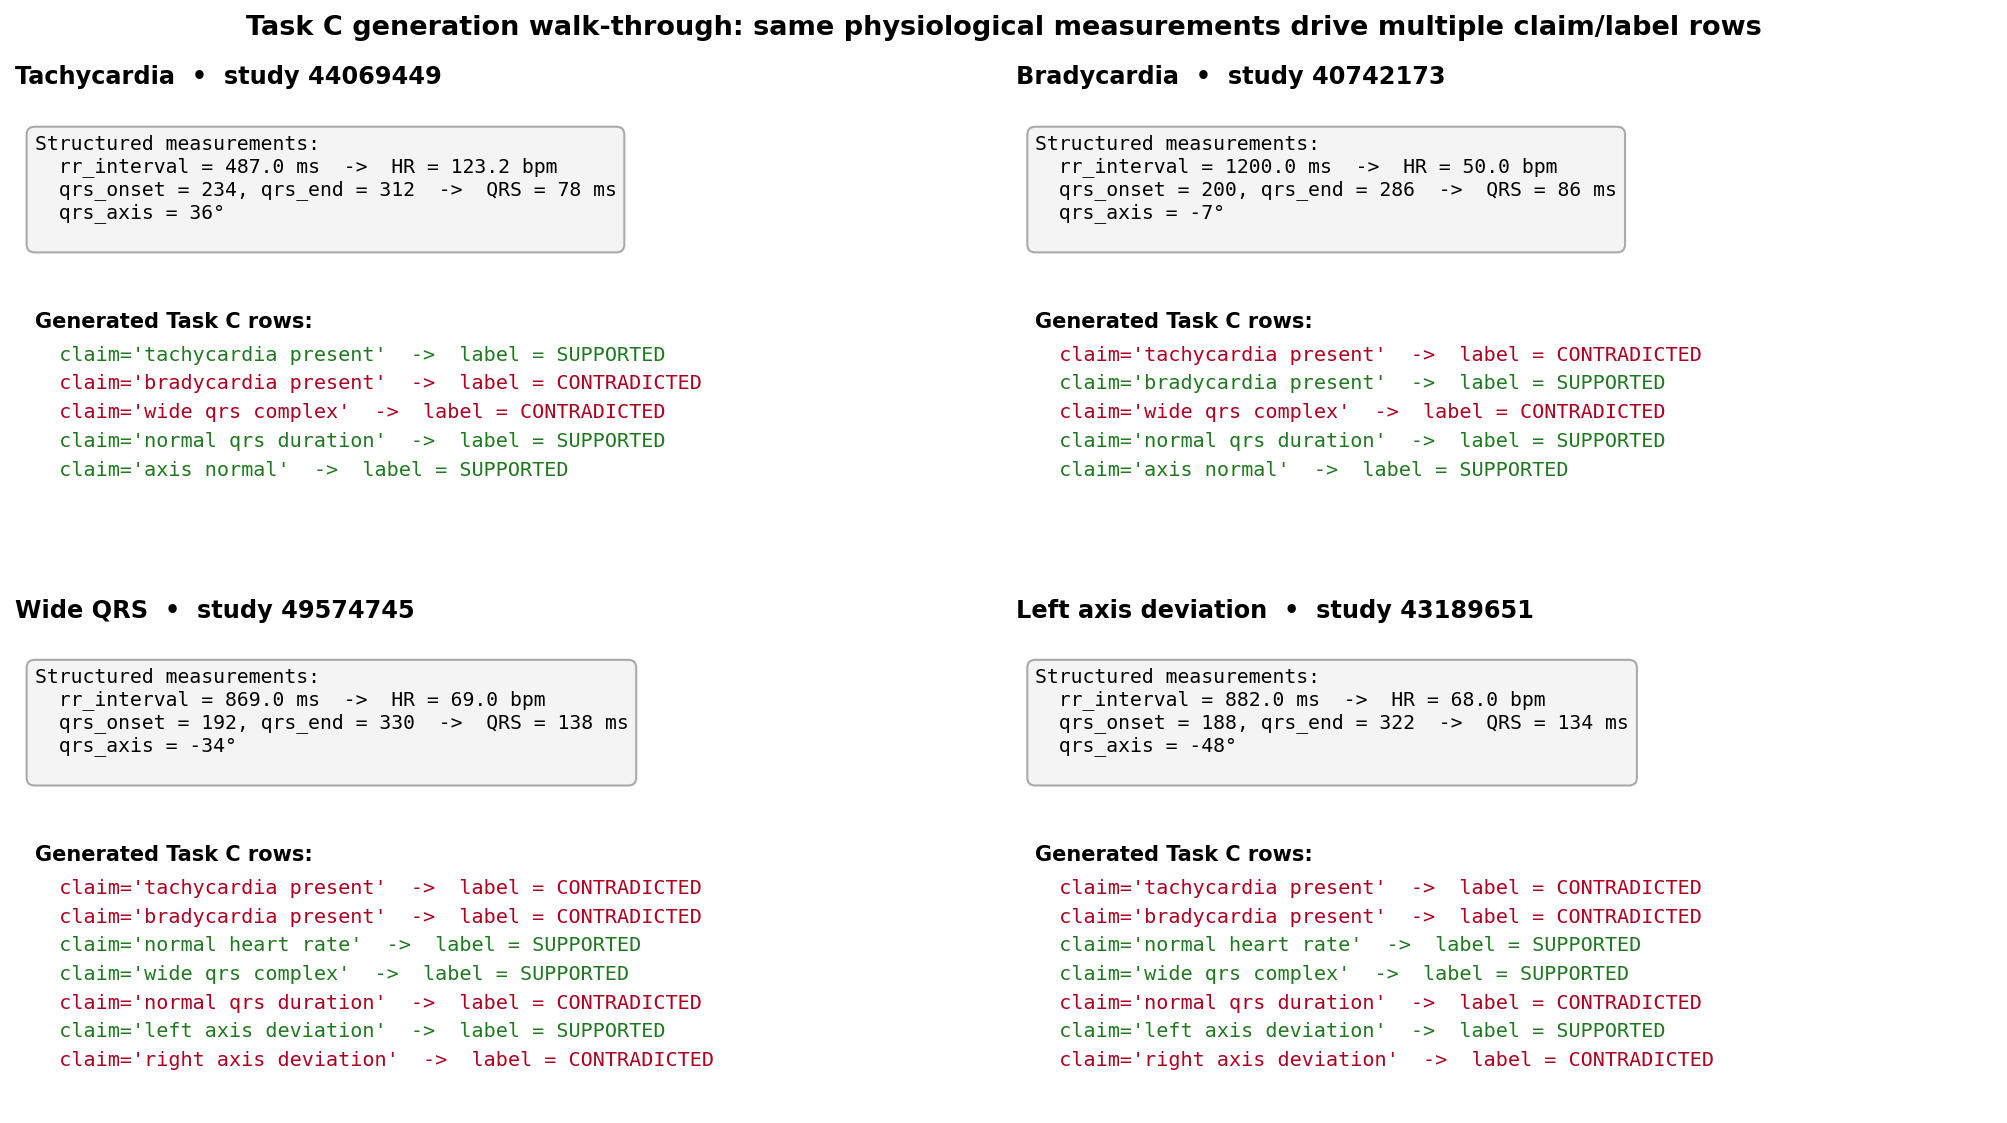
\includegraphics[width=\linewidth]{fig_taskC_walkthrough.png}
 \caption{Task~C generation walk-through. Each panel reproduces \texttt{task\_C.py}'s logic on a real cleaned study, prints the structured measurements that drive the claims, and shows the (claim, label) rows that the script writes to JSONL. The four condition branches (tachy, brady, wide QRS, axis) cover all eight claim strings.}
 \label{fig:taskC_walkthrough}
\end{figure}

\begin{figure}[!ht]
 \centering
 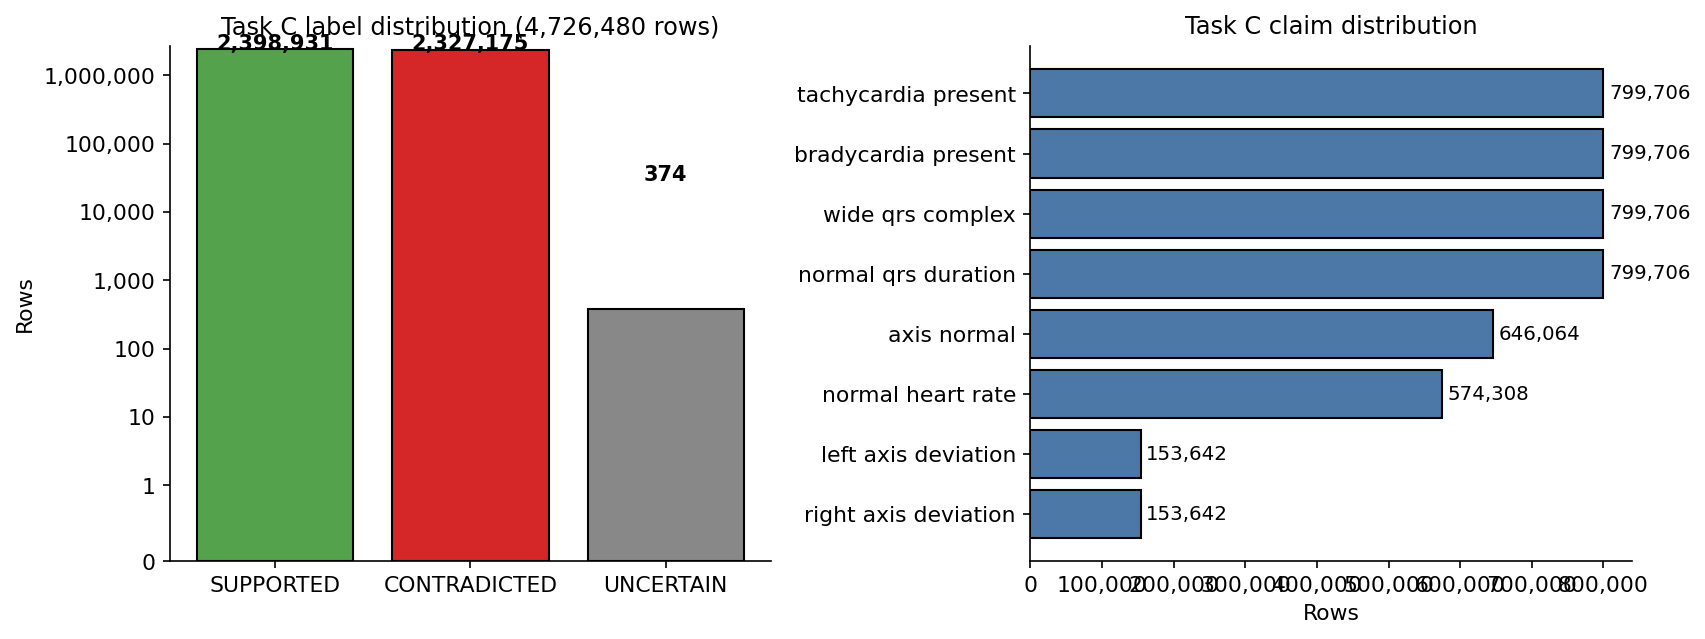
\includegraphics[width=\linewidth]{fig_taskC_distribution.png}
 \caption{Task~C label and claim distribution computed by streaming \texttt{taskC\_plausibility.jsonl}. Left: SUPPORTED, CONTRADICTED, and UNCERTAIN counts on a symmetric-log $y$-axis, so the small UNCERTAIN bar (374 rows from invalid RR) is still visible. Right: per-claim row count.}
 \label{fig:taskC_distribution}
\end{figure}

\begin{figure}[!ht]
 \centering
 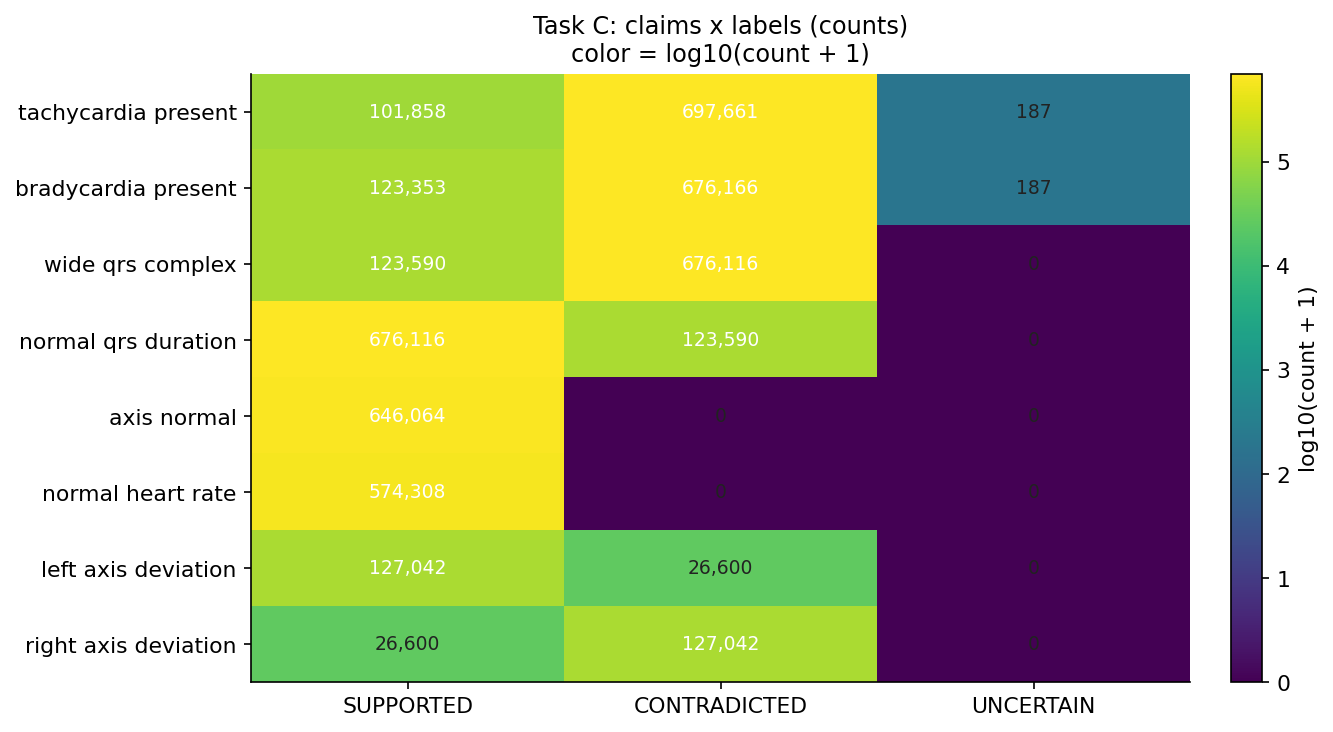
\includegraphics[width=0.8\linewidth]{fig_taskC_heatmap.png}
 \caption{Task~C claim$\times$label heatmap (color = $\log_{10}(\text{count}+1)$). Every claim has non-trivial \texttt{SUPPORTED} mass; the four heart-rate / QRS claims also have many \texttt{CONTRADICTED} rows because they are emitted as the inverse of the matching SUPPORTED row from the same measurement. UNCERTAIN appears only on the two heart-rate claims (the $187$ studies with invalid RR contribute $374$ rows).}
 \label{fig:taskC_heatmap}
\end{figure}

\section*{Data Records}

\subsection*{File layout}

The Tri-Modal-ECG dataset is organised under \texttt{processed/} of the project repository (Listing~\ref{lst:layout}). Top-level directories carry one file per study, named by \texttt{study\_id}. Three Apache Parquet indexes describe the dataset at increasing levels of curation; three JSONL files carry the benchmark tasks; per-study QC JSONs persist the validity of every record.

\begin{lstlisting}[caption={On-disk layout of the released dataset.},label={lst:layout},language=,basicstyle=\ttfamily\scriptsize]
processed/
  index/
    index.parquet                          (800,035 rows)
    index_with_split.parquet               (800,033 rows + train/val/test)
    index_clean.parquet                    (799,706 rows; tri-modal valid)
    index_clean_with_measurements.parquet  (+ rr_interval, p_*, qrs_*, t_* axes)
    splits.json                            (patient ID lists per split)
  signals_lead2/{study_id}.npy             (length-5000 float, 16.5 GB)
  signals_12lead/{study_id}.npy            (5000x12 float, 196.6 GB)
  signal_metadata/{study_id}.json          (lead names, sampling rate, ...)
  images_clean/{study_id}.png              (Matplotlib clean PNG, 147.6 GB)
  images_scanlike/{study_id}.jpg           (deterministic scan-like JPG, 71.6 GB)
  qc/{study_id}.json                       (waveform/image/text validity)
  taskA_verification.jsonl                 (5,597,755 rows, 995 MB)
  taskA_stats.json                         (per-negative-type counts)
  taskB_temporal_grounding.jsonl           (2,399,118 rows, 262 MB)
  taskC_plausibility.jsonl                 (4,726,480 rows, 451 MB)
\end{lstlisting}

\subsection*{Modality alignment and storage}

Each cleaned study is jointly addressable by its \texttt{study\_id} across all four modalities. Figure~\ref{fig:modality_montage} shows one record's four artefacts side-by-side as a ``data card''. Storage is dominated by the lossless 12-lead arrays and the clean PNGs (Figure~\ref{fig:storage}); the scan-like JPGs are $\approx$48\% the size of the corresponding PNGs even after the augmentation chain, and the Lead~II-only arrays are an order of magnitude smaller than the 12-lead arrays. Table~\ref{tab:storage} reports the per-modality file count and total bytes.

\begin{figure}[!ht]
 \centering
 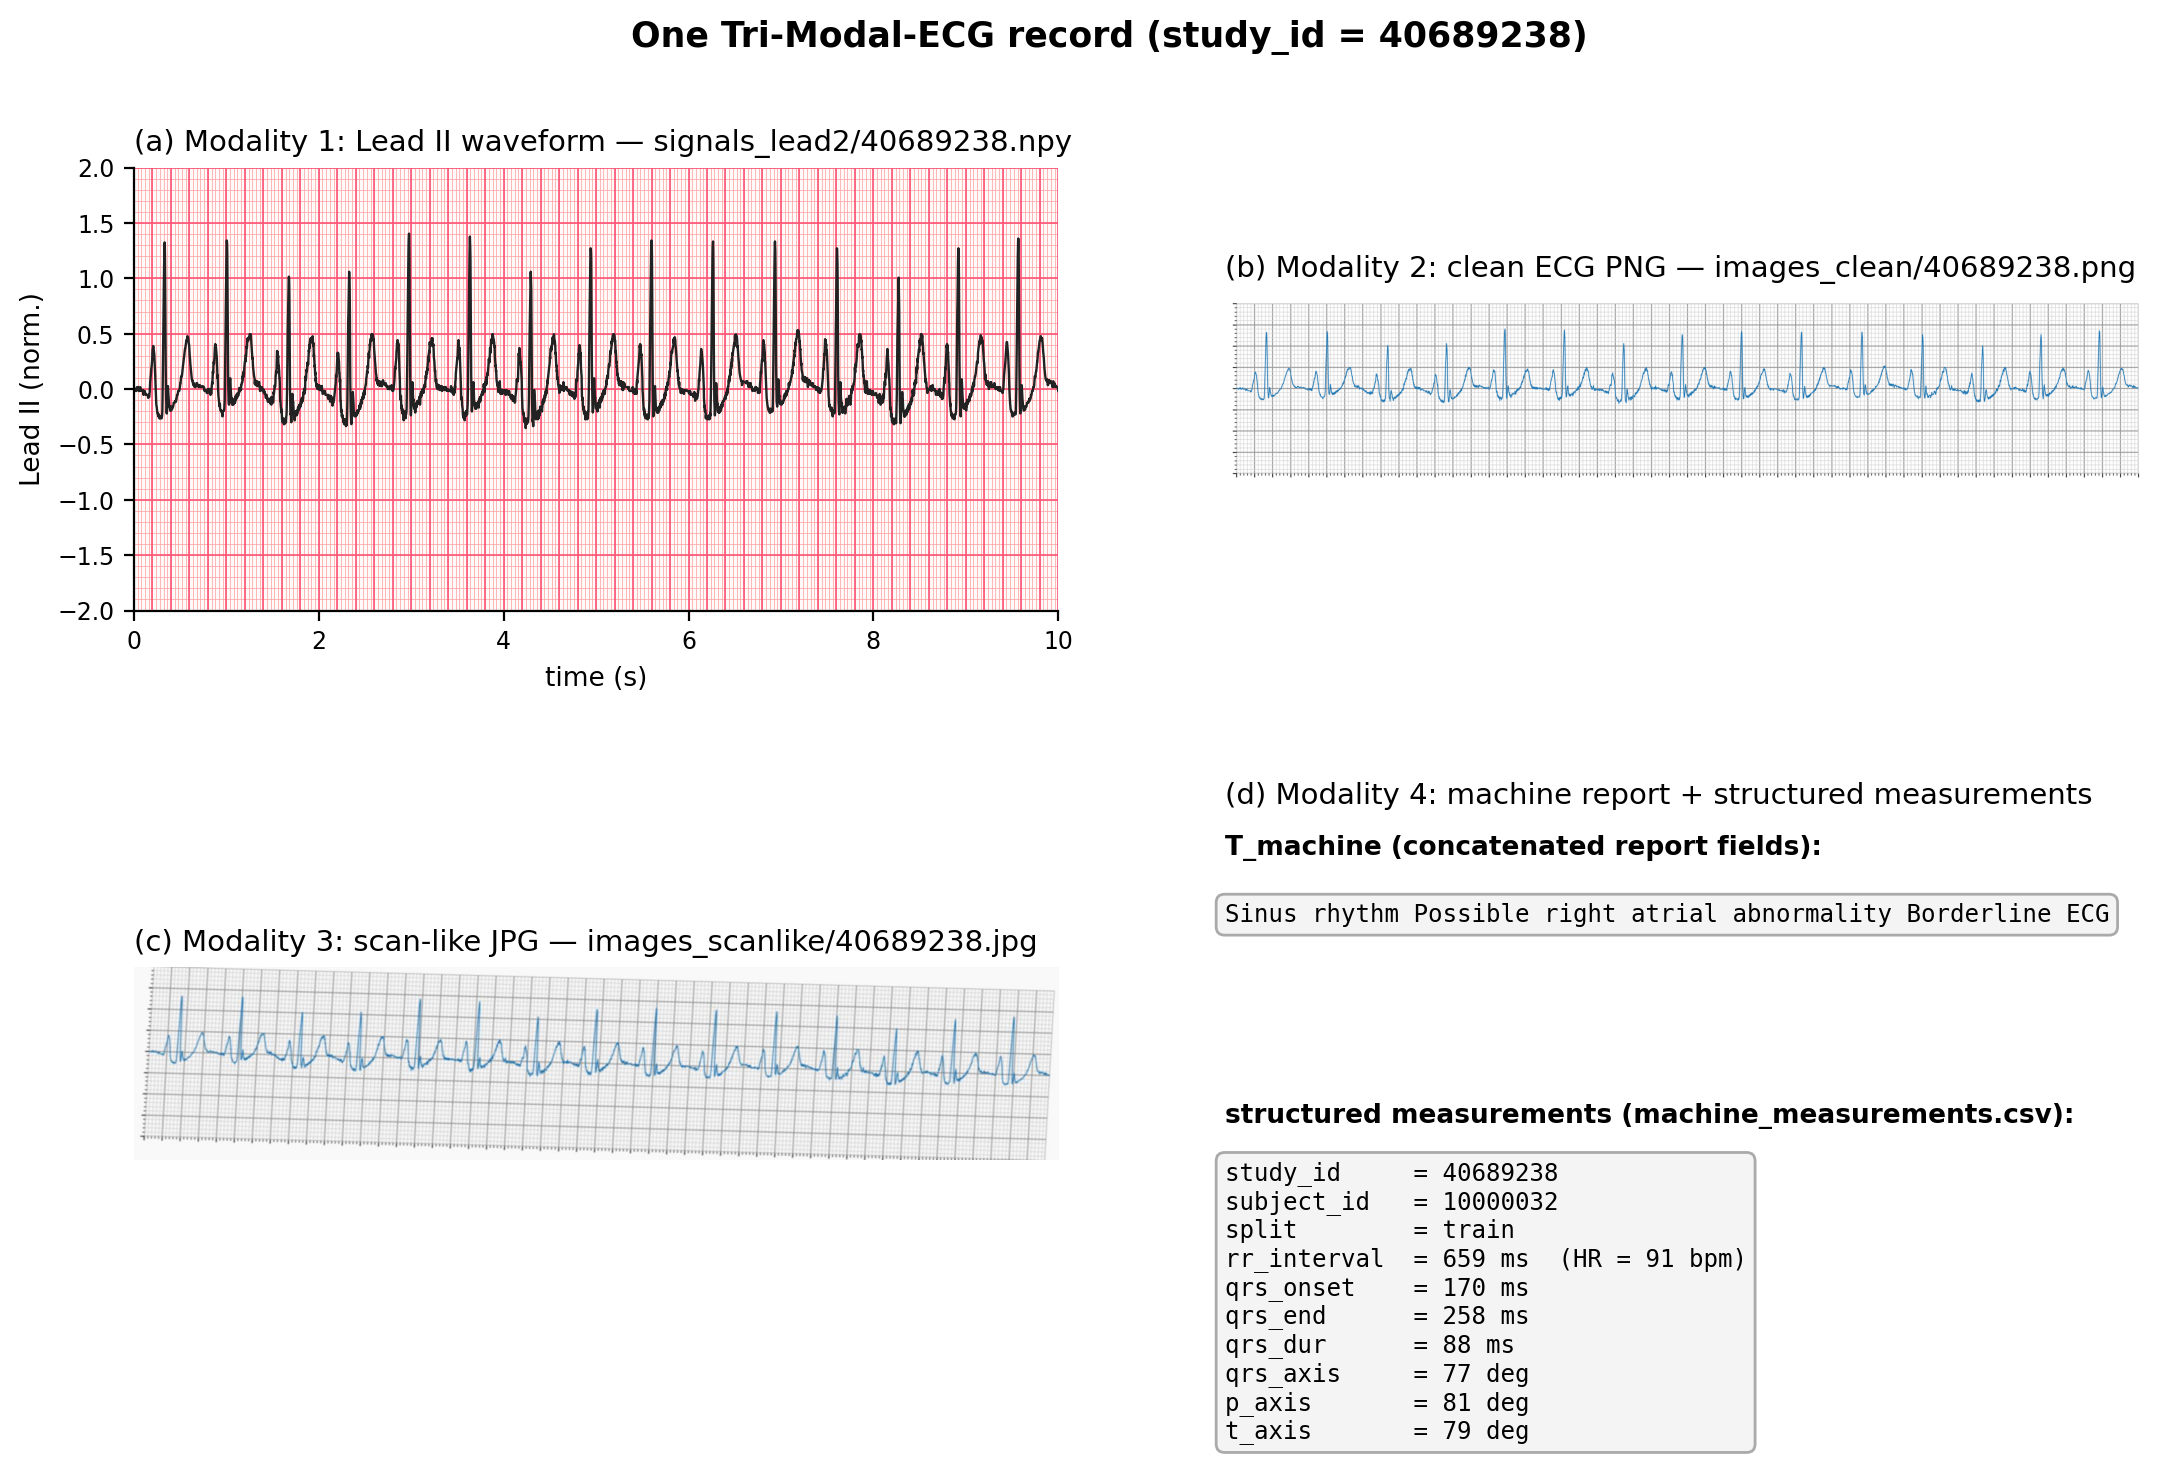
\includegraphics[width=\linewidth]{fig_modality_montage.png}
 \caption{One Tri-Modal-ECG record viewed across its four modalities (study \texttt{40689238}, \texttt{normal\_high} HR group). (a) Lead~II waveform array. (b) Clean ECG-paper PNG rendered from (a). (c) Scan-like JPG produced deterministically from (b). (d) The MIMIC-IV machine report and the structured measurements joined into the cleaned index. All four artefacts share the same \texttt{study\_id}.}
 \label{fig:modality_montage}
\end{figure}

\begin{figure}[!ht]
 \centering
 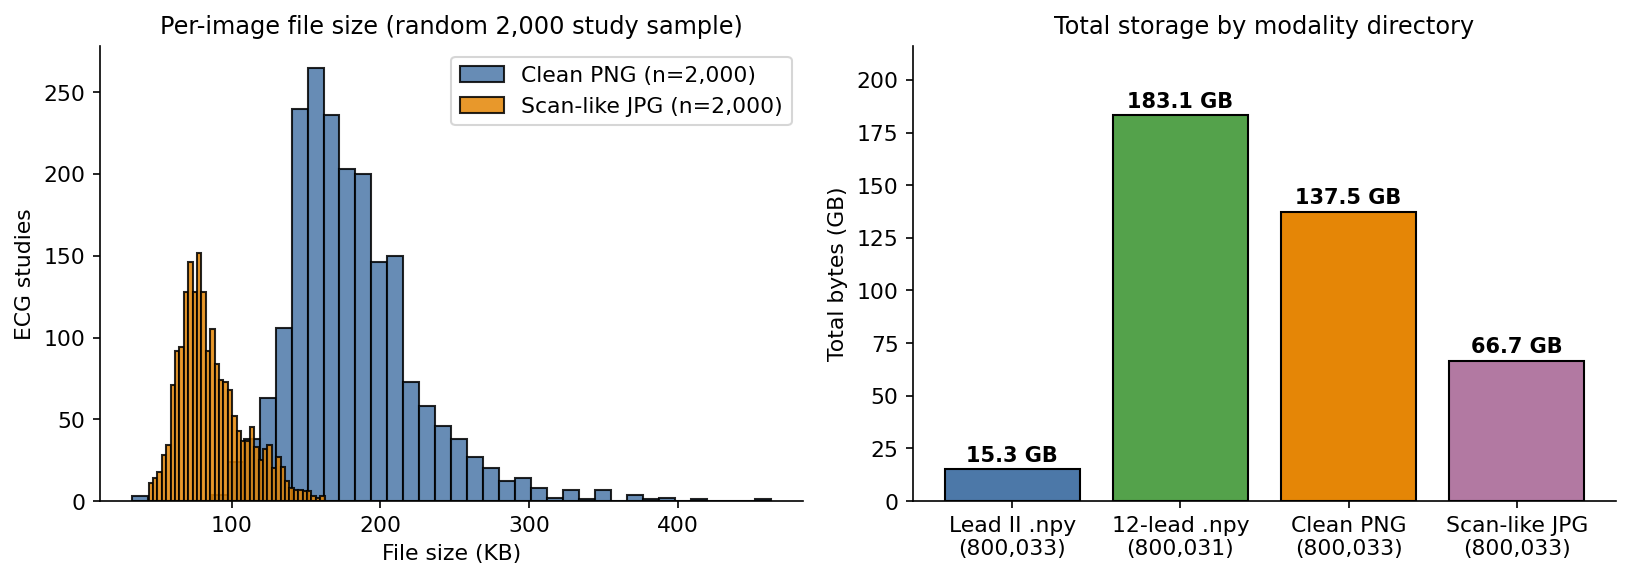
\includegraphics[width=\linewidth]{fig_storage_comparison.png}
 \caption{Storage footprint by modality. Left: per-image file size distribution (2{,}000 randomly sampled studies). Right: total bytes per directory after deduplication. Lossless PNGs dominate the on-disk footprint; the JPEG-encoded scan-like images are roughly half the size despite the per-study augmentation chain.}
 \label{fig:storage}
\end{figure}

\begin{table}[!ht]
\centering
\caption{Per-modality file count and total bytes for the released dataset. The lower file count for QC and signal metadata (each $800{,}033$) reflects the post-split index size; the cleaned tri-modal index ($799{,}706$ rows) is a strict subset.}
\label{tab:storage}
\renewcommand{\arraystretch}{1.25}
\begin{tabular}{l r r}
\toprule
Directory / file & Files & Total bytes \\
\midrule
\texttt{signals\_lead2/}                  & 800{,}033 &  16{,}472{,}663{,}136 \\
\texttt{signals\_12lead/}                 & 800{,}031 & 196{,}615{,}360{,}384 \\
\texttt{signal\_metadata/}                & 781{,}230 & 79{,}708{,}082 \\
\texttt{images\_clean/}                   & 800{,}033 & 147{,}623{,}940{,}034 \\
\texttt{images\_scanlike/}                & 800{,}033 &  71{,}565{,}027{,}783 \\
\texttt{qc/}                              & 800{,}033 & 72{,}808{,}556 \\
\texttt{taskA\_verification.jsonl}        & 1 file (5{,}597{,}755 rows) & 995{,}525{,}090 \\
\texttt{taskB\_temporal\_grounding.jsonl} & 1 file (2{,}399{,}118 rows) & 261{,}586{,}328 \\
\texttt{taskC\_plausibility.jsonl}        & 1 file (4{,}726{,}480 rows) & 450{,}748{,}659 \\
\bottomrule
\end{tabular}
\end{table}

\subsection*{Index schemas}

Table~\ref{tab:index_schema} summarises the columns shipped with the cleaned, measurement-enriched index. Tables~\ref{tab:taskA_schema}, \ref{tab:taskB_schema}, \ref{tab:taskC_schema} describe the JSONL row schema for the three benchmark tasks.

\begin{table}[!ht]
\centering
\caption{Schema of \texttt{index\_clean\_with\_measurements.parquet} (799{,}706 rows). All columns are sourced from MIMIC-IV-ECG except \texttt{split}, which is assigned by our patient-level partitioner.}
\label{tab:index_schema}
\renewcommand{\arraystretch}{1.2}
\begin{tabular}{@{}l l p{0.55\linewidth}@{}}
\toprule
Column & Type & Description \\
\midrule
\texttt{study\_id}    & int64  & MIMIC-IV-ECG study identifier (primary key) \\
\texttt{subject\_id}  & int64  & MIMIC-IV patient identifier \\
\texttt{path}         & string & Relative WFDB path inside \texttt{data/files/} \\
\texttt{T\_machine}   & string & Concatenation of \texttt{report\_0}--\texttt{report\_17} from the MIMIC release \\
\texttt{split}        & string & One of \texttt{train}, \texttt{val}, \texttt{test} (assigned per patient) \\
\texttt{rr\_interval} & float  & RR interval (ms) \\
\texttt{p\_onset}, \texttt{p\_end}     & float & P-wave timing (ms) \\
\texttt{qrs\_onset}, \texttt{qrs\_end} & float & QRS-complex timing (ms) \\
\texttt{t\_end}       & float  & End of T wave (ms) \\
\texttt{p\_axis}, \texttt{qrs\_axis}, \texttt{t\_axis} & float & Electrical axes (deg.) \\
\bottomrule
\end{tabular}
\end{table}

\begin{table}[!ht]
\centering
\caption{Schema of one row in \texttt{taskA\_verification.jsonl}.}
\label{tab:taskA_schema}
\renewcommand{\arraystretch}{1.2}
\begin{tabular}{l l p{0.55\linewidth}}
\toprule
Field & Type & Description \\
\midrule
\texttt{anchor\_study\_id} & int   & Anchor study \\
\texttt{signal\_id}        & int   & \texttt{study\_id} contributing the Lead~II signal \\
\texttt{image\_id}         & int   & \texttt{study\_id} contributing the image \\
\texttt{text\_id}          & int   & \texttt{study\_id} contributing the text report \\
\texttt{image\_type}       & string & \texttt{clean} or \texttt{scanlike} \\
\texttt{y\_match}          & int (0/1) & 1 if all three IDs equal the anchor \\
\texttt{neg\_type}         & string or null & One of \texttt{TEXT\_SWAP}, \texttt{IMAGE\_SWAP}, \texttt{SIGNAL\_SWAP}, \texttt{PARTIAL\_MISMATCH}, \texttt{HARD\_NEGATIVE\_TEXT}; \texttt{null} for positives \\
\texttt{split}             & string & Inherited from the anchor's patient split \\
\bottomrule
\end{tabular}
\end{table}

\begin{table}[!ht]
\centering
\caption{Schema of one row in \texttt{taskB\_temporal\_grounding.jsonl}. Each row carries a length-10 binary vector, one per one-second bin.}
\label{tab:taskB_schema}
\renewcommand{\arraystretch}{1.2}
\begin{tabular}{l l p{0.55\linewidth}}
\toprule
Field & Type & Description \\
\midrule
\texttt{study\_id} & int    & Cleaned study identifier \\
\texttt{query}     & string & One of \texttt{HIGH\_HEART\_RATE}, \texttt{LOW\_HEART\_RATE}, \texttt{WIDE\_QRS} \\
\texttt{labels}    & list[int] (length 10) & 1 if the bin satisfies the query (local detection), else 0 \\
\texttt{split}     & string & Inherited from the patient split \\
\bottomrule
\end{tabular}
\end{table}

\begin{table}[!ht]
\centering
\caption{Schema of one row in \texttt{taskC\_plausibility.jsonl}.}
\label{tab:taskC_schema}
\renewcommand{\arraystretch}{1.2}
\begin{tabular}{l l p{0.55\linewidth}}
\toprule
Field & Type & Description \\
\midrule
\texttt{study\_id} & int    & Cleaned study identifier \\
\texttt{claim}     & string & One of eight claim strings (see text) \\
\texttt{label}     & string & \texttt{SUPPORTED}, \texttt{CONTRADICTED}, or \texttt{UNCERTAIN} \\
\texttt{split}     & string & Inherited from the patient split \\
\bottomrule
\end{tabular}
\end{table}

\subsection*{Reading the dataset}

Below is a minimal Python snippet that opens the four modalities of one record together. The snippet does not require any custom library: NumPy \cite{harris2020array}, Pillow, and pandas with PyArrow \cite{vaynberg2020apache} cover the full read path.

\begin{lstlisting}[caption={Reading one Tri-Modal-ECG record across all four modalities.},label={lst:reader},language=Python]
import json
import numpy as np
import pandas as pd
from PIL import Image

ROOT = "processed"
study_id = 40689238

# 1. Lead-II waveform (length 5000, 500 Hz)
sig_lead2 = np.load(f"{ROOT}/signals_lead2/{study_id}.npy")

# 2. 12-lead waveform (5000 x 12)
sig_12lead = np.load(f"{ROOT}/signals_12lead/{study_id}.npy")

# 3. Clean ECG-paper PNG
img_clean = Image.open(f"{ROOT}/images_clean/{study_id}.png")

# 4. Deterministic scan-like JPG
img_scan = Image.open(f"{ROOT}/images_scanlike/{study_id}.jpg")

# 5. Aligned text + structured measurements
df = pd.read_parquet(f"{ROOT}/index/index_clean_with_measurements.parquet")
row = df[df.study_id == study_id].iloc[0]
print(row.T_machine)
print({c: row[c] for c in ["rr_interval", "qrs_onset", "qrs_end", "qrs_axis"]})

# 6. Per-study QC status
with open(f"{ROOT}/qc/{study_id}.json") as fp:
    print(json.load(fp))
\end{lstlisting}

\section*{Technical Validation}

Technical validation has three components: (i) coverage and integrity of the released artefacts, (ii) descriptive statistics of the structured measurements compared with expected physiological ranges, and (iii) per-task validation of the three benchmark JSONLs.

\subsection*{Coverage and dataset funnel}

The dataset funnel from the raw \texttt{record\_list.csv} to the final cleaned tri-modal index removes 329 studies, every one of which corresponds to a missing or invalid modality (Figure~\ref{fig:funnel}). The post-QC patient-level split is shown in Table~\ref{tab:split} and the per-modality file coverage in Figure~\ref{fig:modality_coverage}. The persisted \texttt{dataset\_integrity\_summary.json} confirms that, of $800{,}035$ expected records, $800{,}033$ have a valid clean PNG and $800{,}033$ have a valid scan-like JPG, and that no decoder failed on any image after the regeneration loop closed (Figure~\ref{fig:regeneration}).

\begin{figure}[!ht]
 \centering
 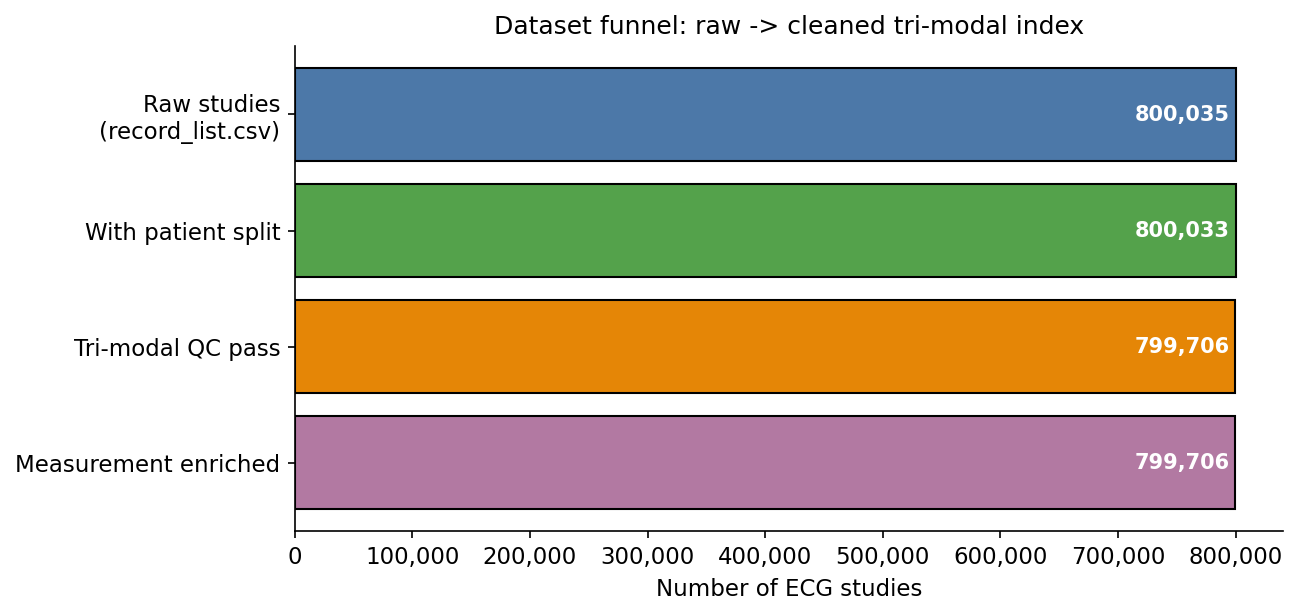
\includegraphics[width=0.7\linewidth]{fig_dataset_funnel.png}
 \caption{Dataset funnel from raw record list ($800{,}035$ studies in MIMIC-IV-ECG) through patient-level split ($800{,}033$), tri-modal QC ($799{,}706$), and measurement enrichment ($799{,}706$). 329 studies are removed in total, each because at least one modality is missing or invalid.}
 \label{fig:funnel}
\end{figure}

\begin{table}[!ht]
\centering
\caption{Patient-level split of the cleaned tri-modal dataset. Patients are pairwise disjoint between splits by construction.}
\label{tab:split}
\renewcommand{\arraystretch}{1.2}
\begin{tabular}{l r r}
\toprule
Split & ECG studies & Unique patients \\
\midrule
Train       & 641{,}053 & 129{,}061 \\
Validation  &  80{,}427 &  16{,}133 \\
Test        &  78{,}226 &  16{,}134 \\
\midrule
Total       & 799{,}706 & 161{,}328 \\
\bottomrule
\end{tabular}
\end{table}

\subsection*{Distribution of structured measurements}

Table~\ref{tab:descriptive} reports central-tendency and dispersion statistics for the structured measurements after suppressing the MIMIC-IV sentinel codes (\texttt{29999, 32767, 65535, $-32768$, $0$}) and applying physiologically-plausible range filters (HR $\in[20,300]$~bpm, $200\leq\text{RR}\leq3000$~ms, $30<\text{P}_\text{dur}<300$~ms, $30<\text{QRS}_\text{dur}<400$~ms, $200<\text{QT}<800$~ms, $|\text{axis}|\leq 180^\circ$). The reported median HR ($74.07$~bpm), median QRS duration ($94$~ms), median QT ($396$~ms) and median QRS axis ($14^\circ$) all sit in the expected adult range and align with values reported by MEETI \cite{zhang2024meeti} on the same upstream measurements.

\begin{table}[!ht]
\centering
\caption{Descriptive statistics of structured measurements (Tri-Modal-ECG cleaned index, $n=799{,}706$). Sentinels and out-of-range values dropped before stats; the ``$n$'' column is the number of remaining valid values. Compare to MEETI \cite{zhang2024meeti} Table~3, which reports similar central tendencies on the same upstream MIMIC-IV-ECG measurements.}
\label{tab:descriptive}
\renewcommand{\arraystretch}{1.25}
\resizebox{\textwidth}{!}{%
\begin{tabular}{l r r r r r r r r}
\toprule
Measurement & $n$ & Mean & Std & Median & IQR & Q1 & Q3 & Range \\
\midrule
HR (bpm)            & 798{,}166 &  78.05 & 20.28 &  74.07 &  24.07 &  64.03 &  88.11 & 20.00, 255.32 \\
RR (ms)             & 798{,}166 & 816.61 & 196.64 & 810.00 & 256.00 & 681.00 & 937.00 & 235.00, 3000.00 \\
P-wave duration (ms) & 568{,}271 & 108.66 &  18.21 & 110.00 &  22.00 &  98.00 & 120.00 & 32.00, 216.00 \\
QRS duration (ms)   & 798{,}104 &  99.72 &  23.07 &  94.00 &  22.00 &  84.00 & 106.00 & 32.00, 391.00 \\
QT interval (ms)    & 798{,}201 & 397.91 &  49.07 & 396.00 &  62.00 & 366.00 & 428.00 & 202.00, 798.00 \\
QRS axis (deg)      & 776{,}506 &  13.28 &  45.38 &  14.00 &  62.00 & $-16.00$ &  46.00 & $-180.00$, 180.00 \\
P axis  (deg)       & 661{,}861 &  45.65 &  29.42 &  51.00 &  31.00 &  33.00 &  64.00 & $-180.00$, 180.00 \\
T axis  (deg)       & 784{,}996 &  40.25 &  56.10 &  42.00 &  51.00 &  16.00 &  67.00 & $-180.00$, 180.00 \\
\bottomrule
\end{tabular}}
\end{table}

\noindent The HR-bucket distribution that drives Task~A and Task~C is shown in Figure~\ref{fig:hr_distribution}; the QRS-duration and QRS-axis distributions that drive Task~C's wide-QRS and axis claims are in Figures~\ref{fig:qrs_duration}--\ref{fig:qrs_axis}. The bucket counts in Figure~\ref{fig:hr_distribution} ($\text{brady}=123{,}353$, $\text{normal\_low}=362{,}372$, $\text{normal\_high}=206{,}115$, $\text{tachy}=107{,}679$, $\text{invalid RR}=187$) sum to the cleaned-index size, confirming that every study is bucketed exactly once.

\begin{figure}[!ht]
 \centering
 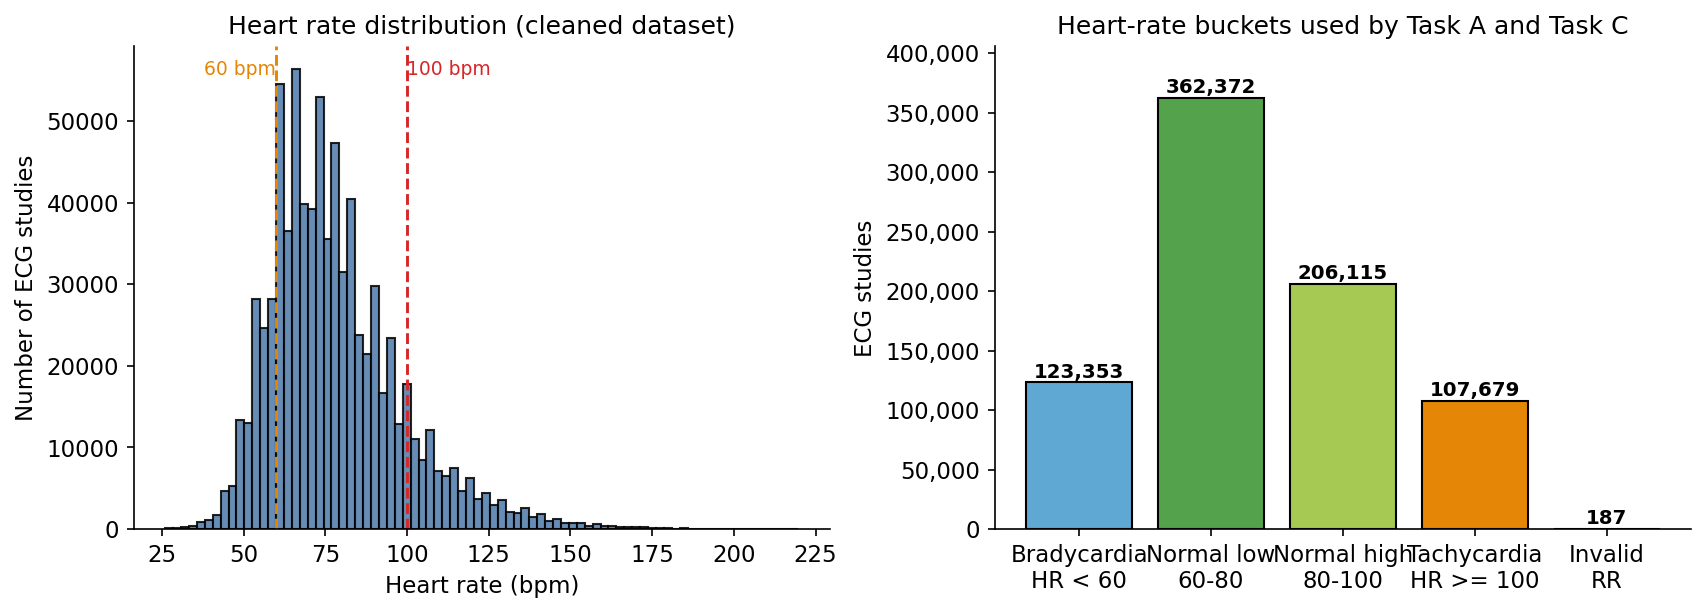
\includegraphics[width=\linewidth]{fig_hr_distribution.png}
 \caption{Heart-rate distribution and the bucket counts used by Task~A and Task~C. Dashed lines mark the 60~bpm and 100~bpm cut-points; bucket counts are written next to the histogram.}
 \label{fig:hr_distribution}
\end{figure}

\begin{figure}[!ht]
 \centering
 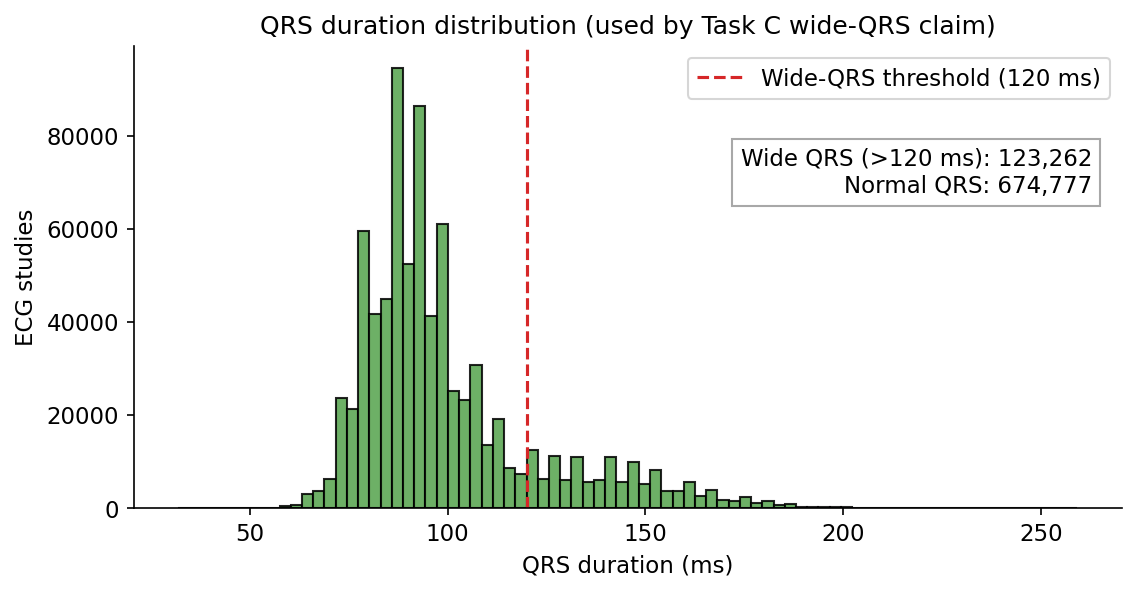
\includegraphics[width=\linewidth]{fig_qrs_duration.png}
 \caption{QRS-duration distribution with the $120$~ms threshold marked. The wide-QRS subset ($n=123{,}590$) is large enough to balance the wide and normal QRS claims in Task~C.}
 \label{fig:qrs_duration}
\end{figure}

\begin{figure}[!ht]
 \centering
 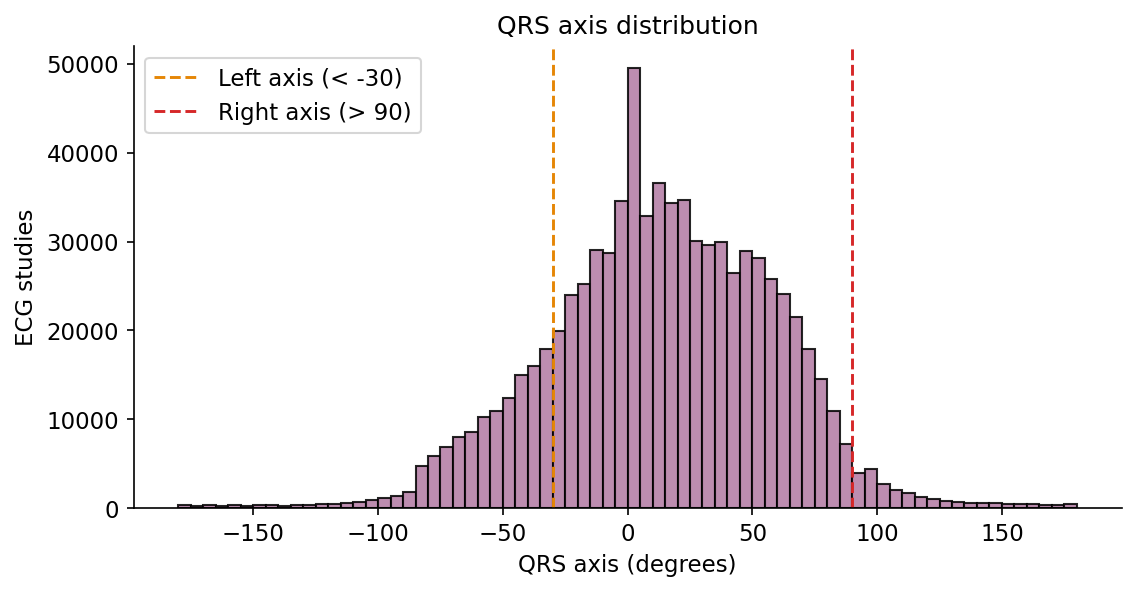
\includegraphics[width=\linewidth]{fig_qrs_axis.png}
 \caption{QRS-axis distribution with the $-30^\circ$ and $+90^\circ$ thresholds. The dataset's distribution shows clear modes around the standard normal-axis range, with a left-axis subset ($127{,}042$ studies) much larger than the right-axis subset ($26{,}600$).}
 \label{fig:qrs_axis}
\end{figure}

\subsection*{Hero examples and axis evidence}

Three ``hero'' figures show the four modalities for representative bradycardia, normal-rhythm, and tachycardia studies, exactly as they will appear to a downstream model (Figures~\ref{fig:hero_brady}--\ref{fig:hero_tachy}); these are the per-study units that Task~A treats as positives. Figure~\ref{fig:axis_examples} presents Lead~II evidence for the three axis branches that drive Task~C's axis claims.

\begin{figure}[!ht]
 \centering
 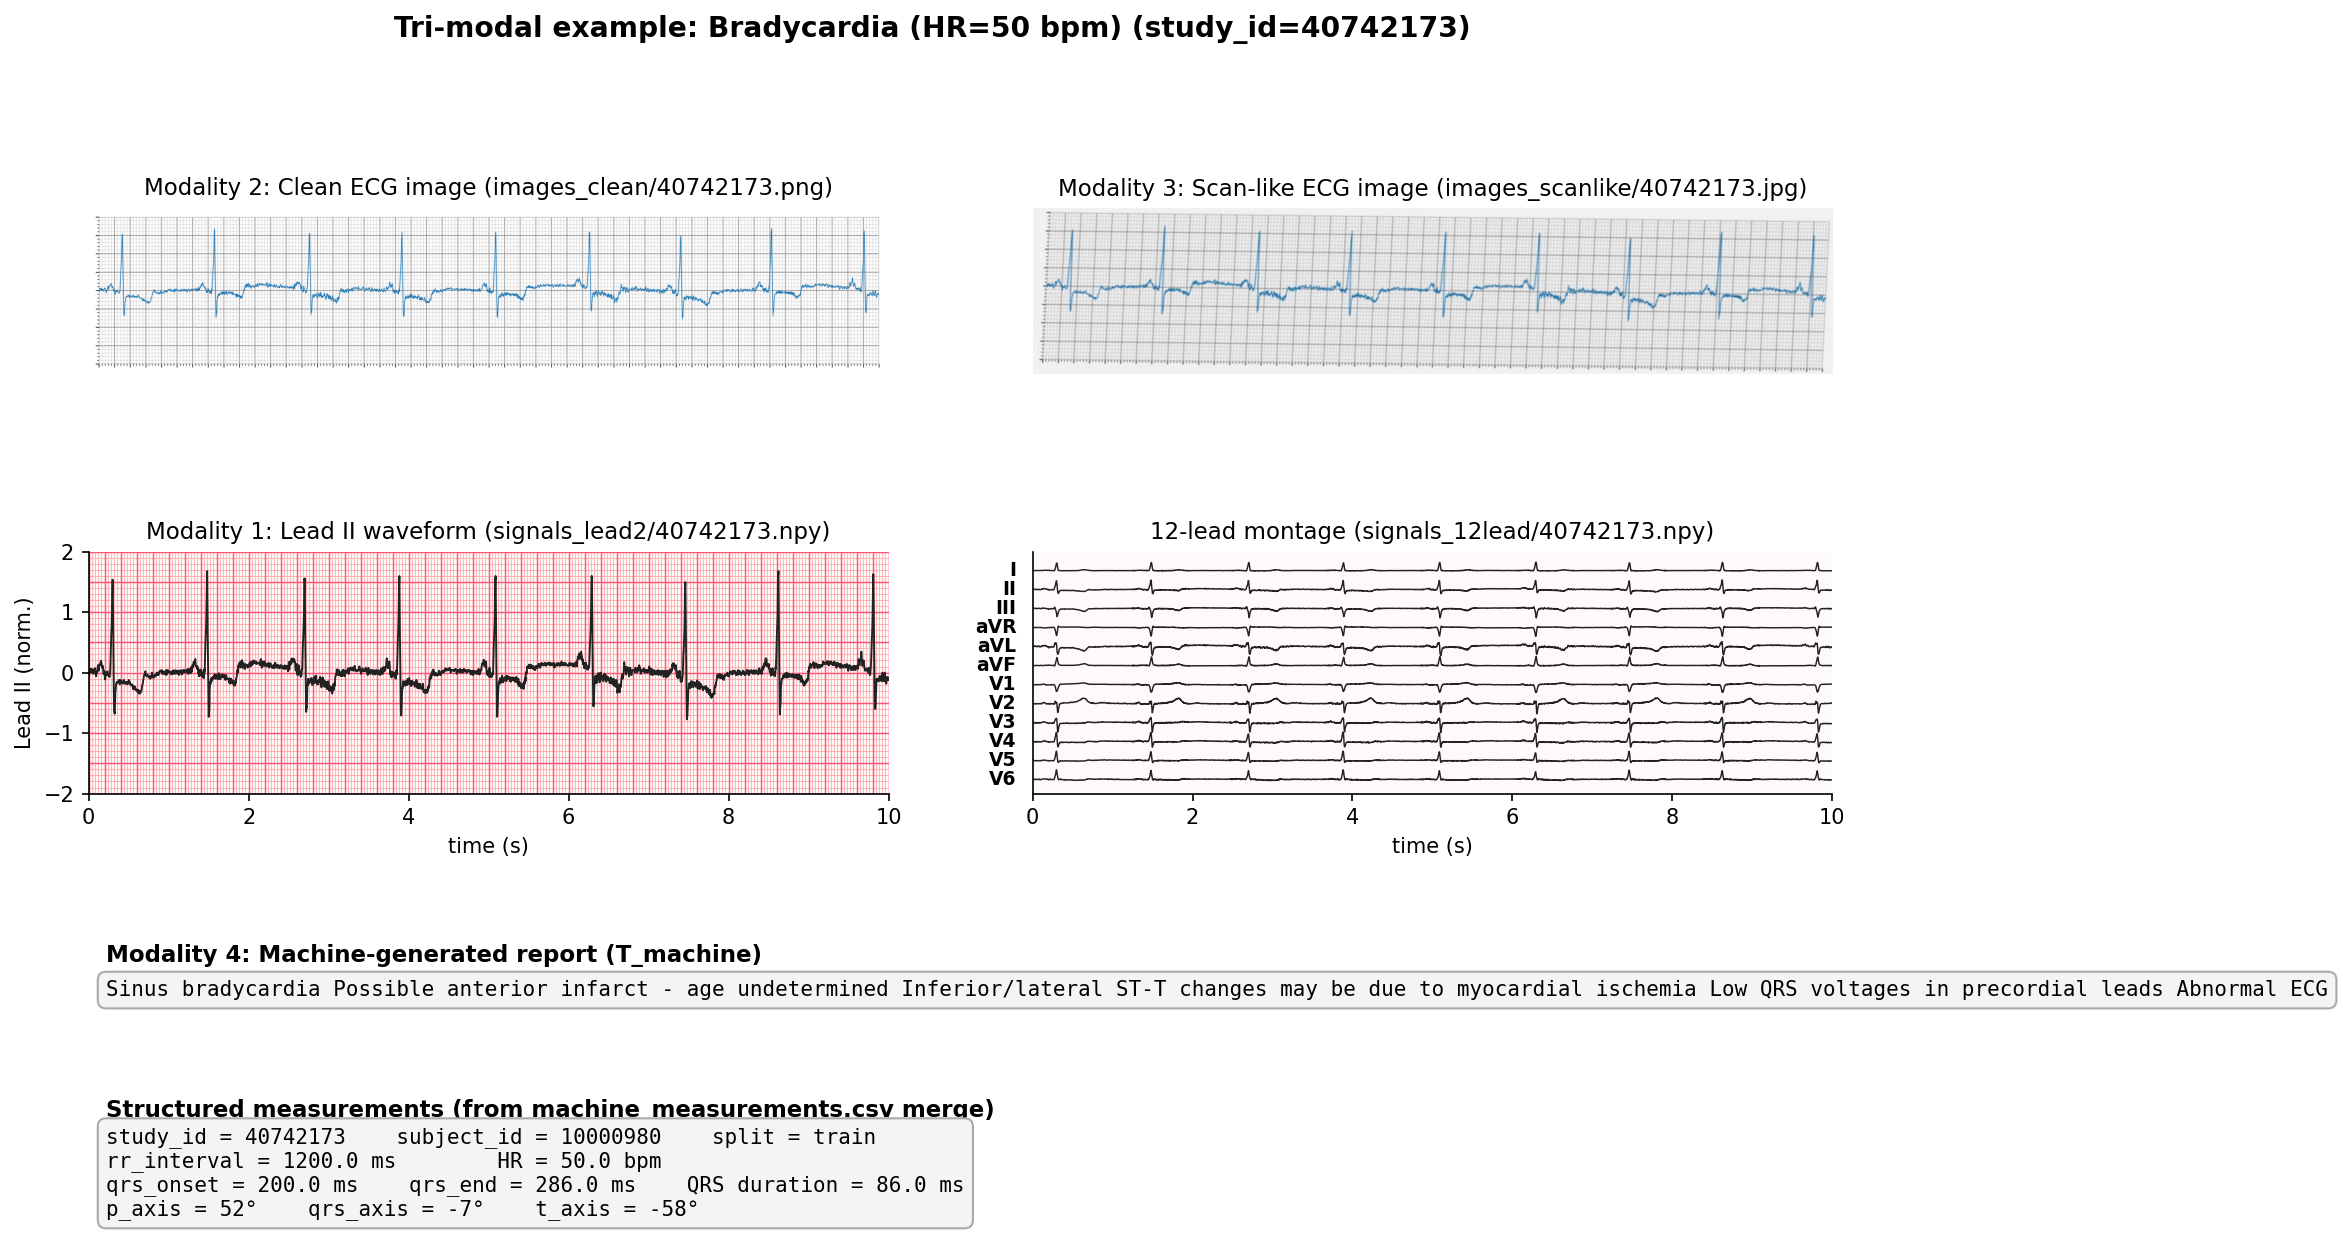
\includegraphics[width=\linewidth]{fig_hero_bradycardia.png}
 \caption{Hero record (bradycardia, HR$=50$~bpm). Top row: Lead~II (left) and 12-lead (right) waveform arrays; bottom row: clean PNG (left) and scan-like JPG (right). The structured-measurement strip on the right matches the Task~C SUPPORTED \texttt{bradycardia present} row that this study contributes.}
 \label{fig:hero_brady}
\end{figure}

\begin{figure}[!ht]
 \centering
 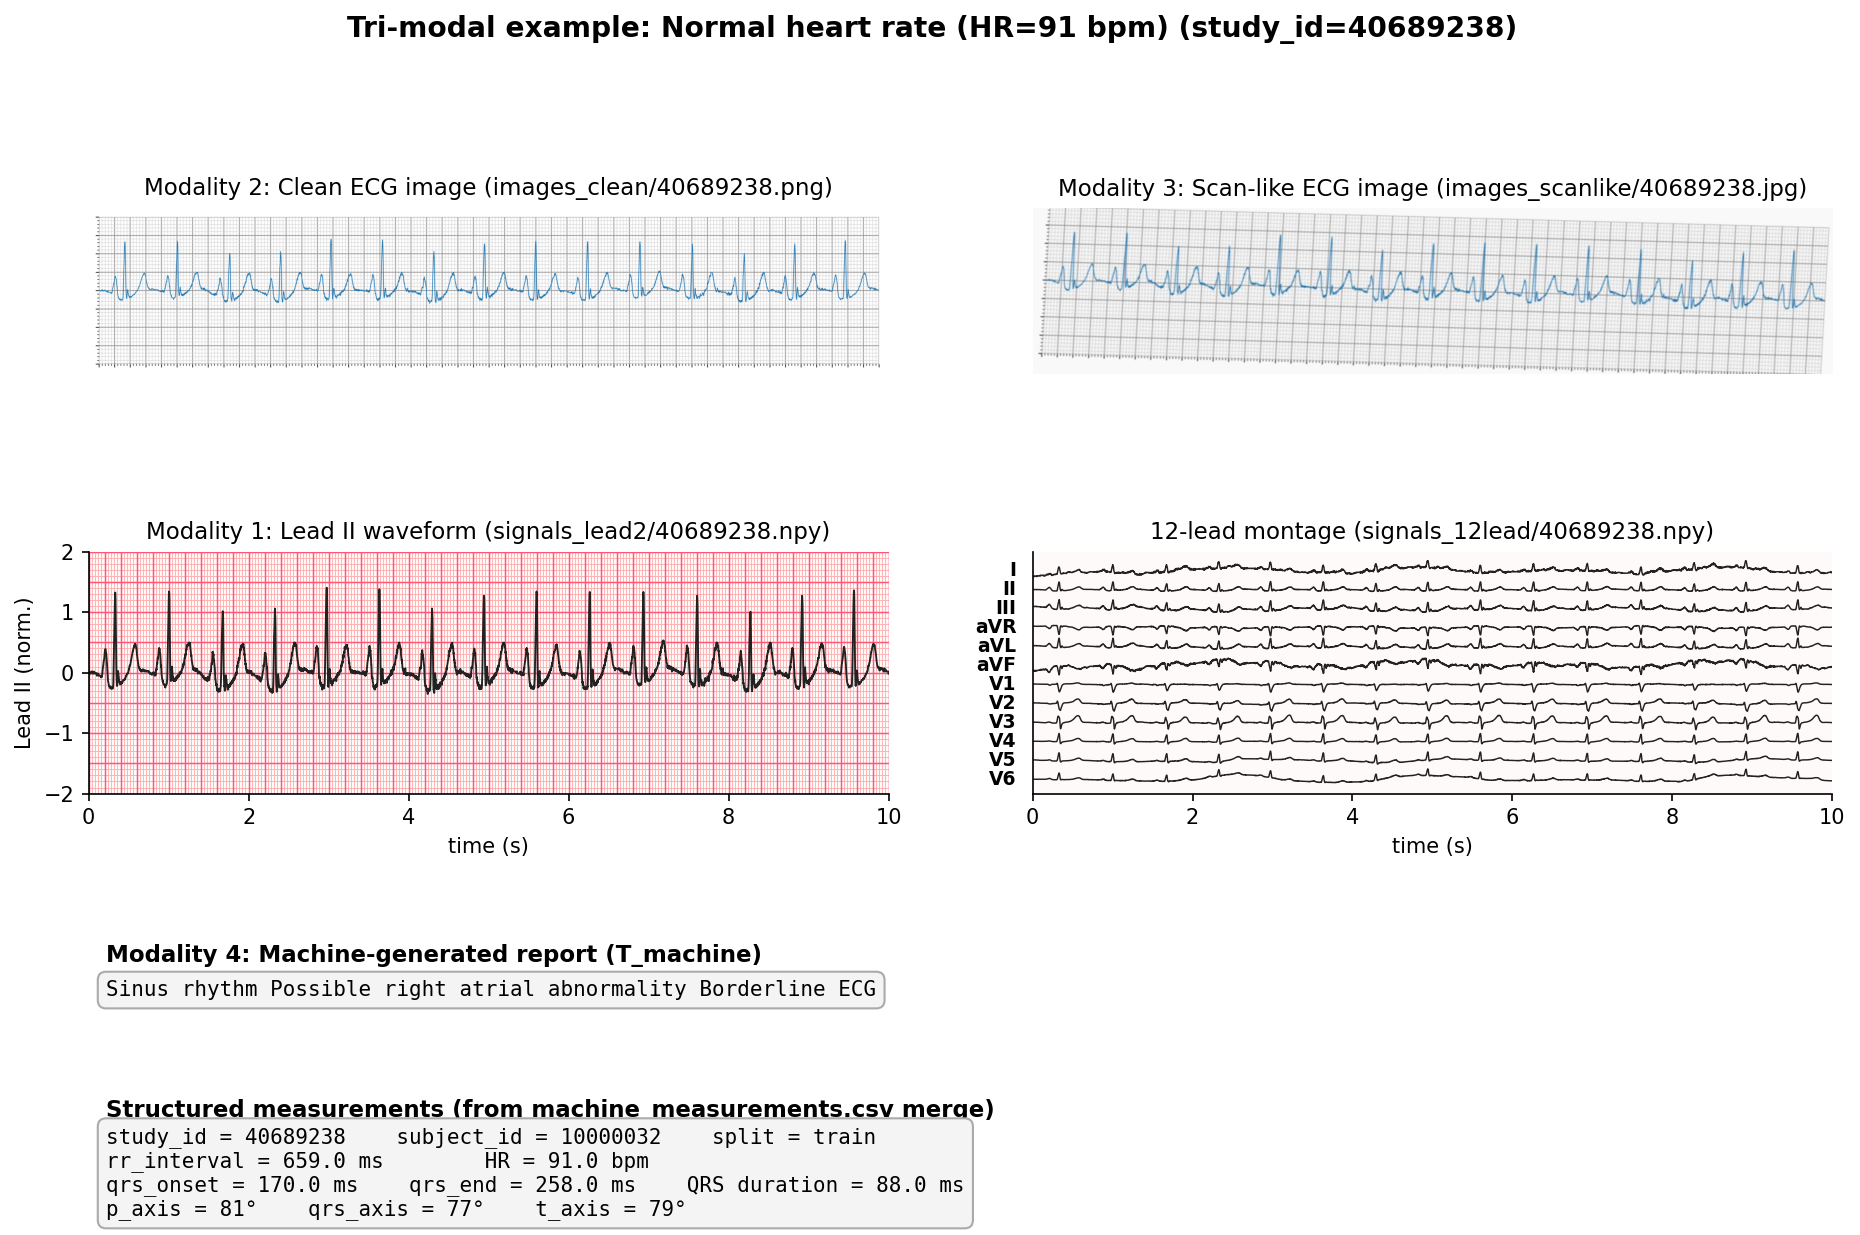
\includegraphics[width=\linewidth]{fig_hero_normal_high.png}
 \caption{Hero record (normal-rhythm, HR$=91$~bpm). The same modality layout as Figure~\ref{fig:hero_brady}; this study contributes Task~C SUPPORTED \texttt{normal heart rate} and \texttt{normal qrs duration} rows.}
 \label{fig:hero_normalhigh}
\end{figure}

\begin{figure}[!ht]
 \centering
 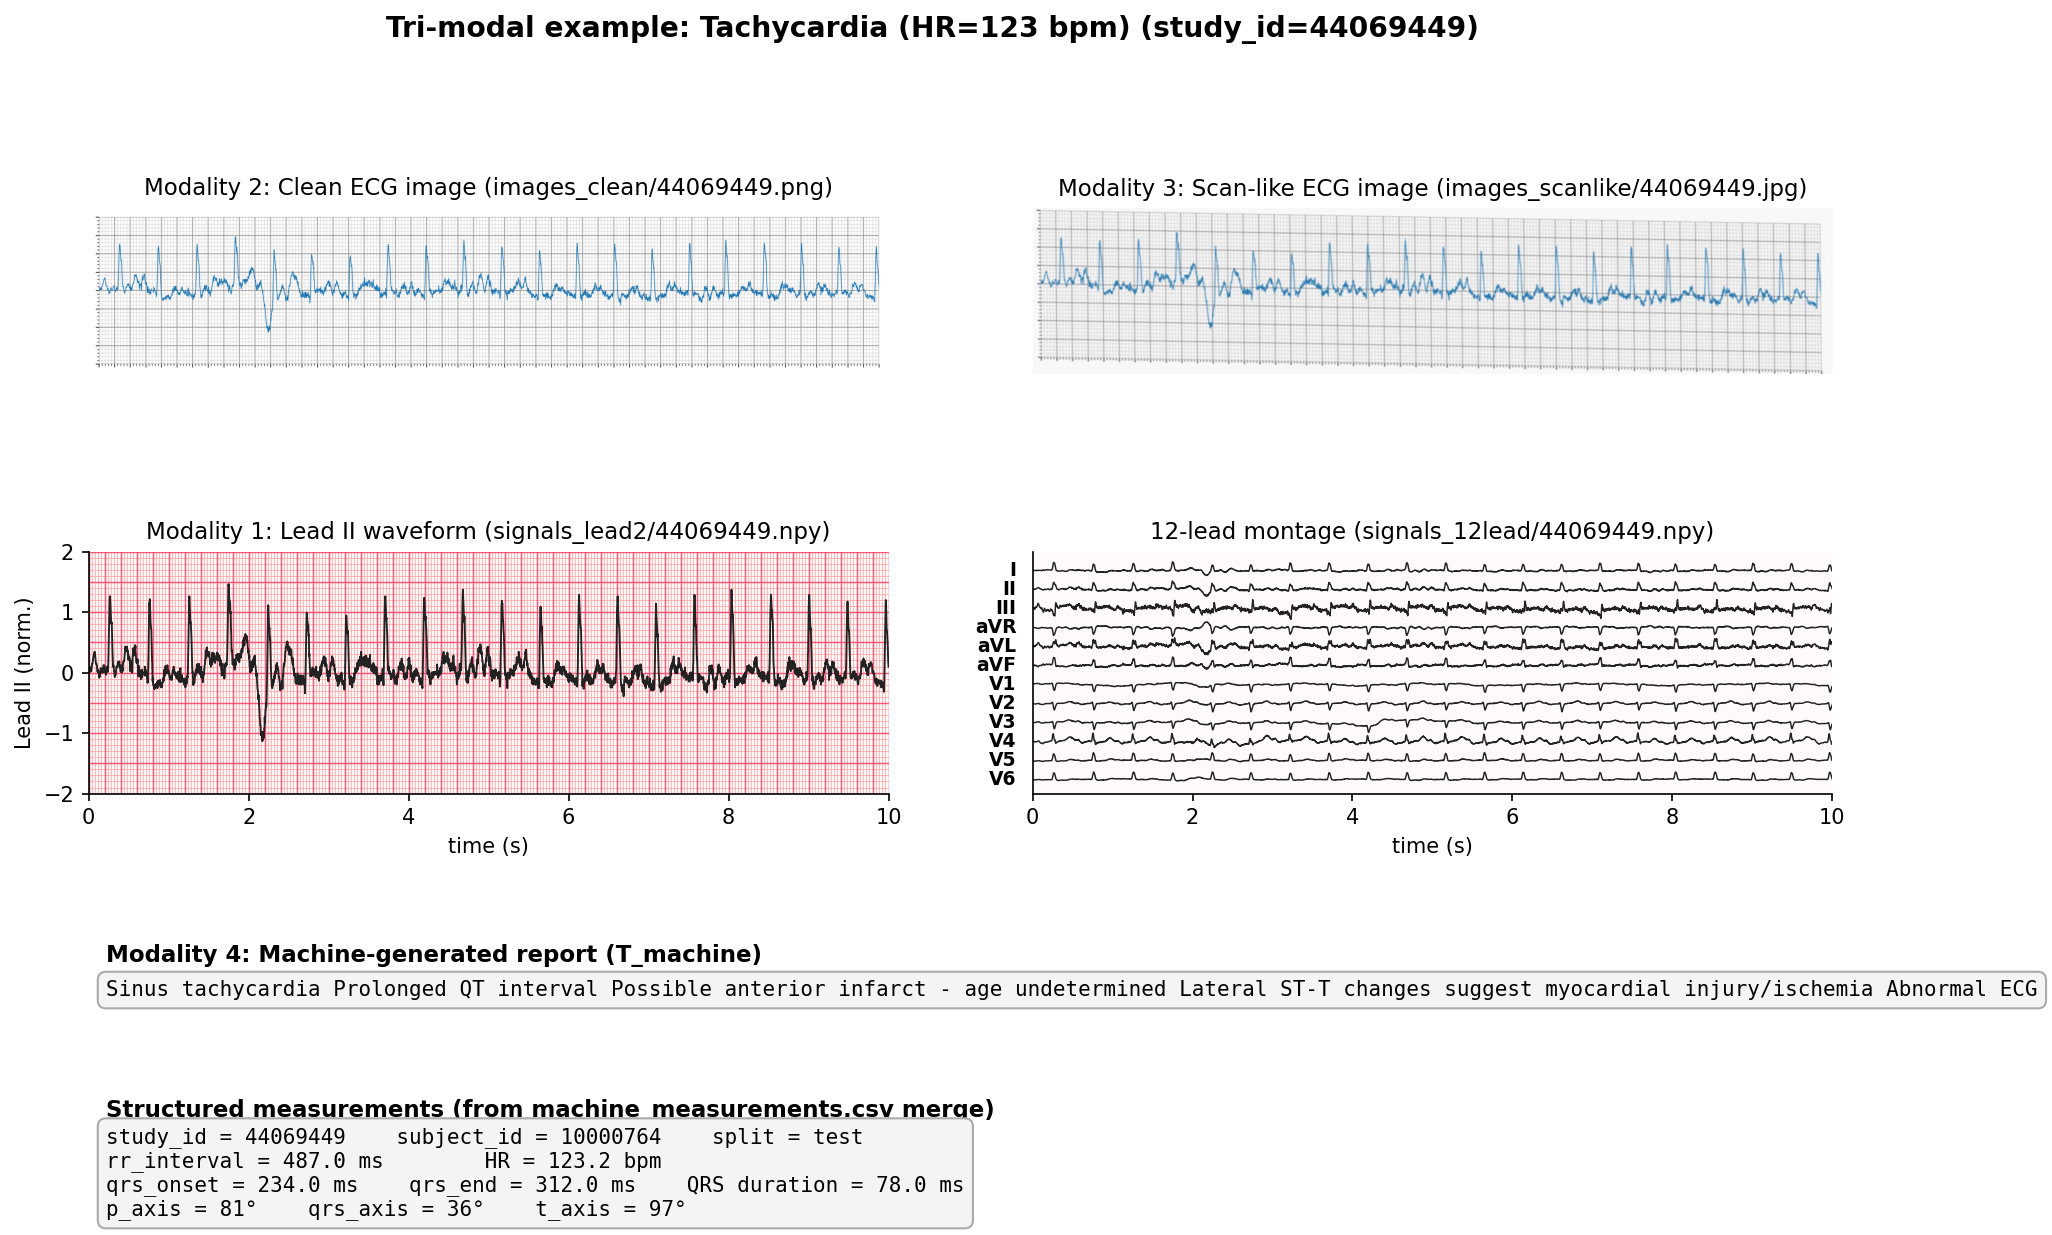
\includegraphics[width=\linewidth]{fig_hero_tachycardia.png}
 \caption{Hero record (tachycardia, HR$=123$~bpm). Same modality layout. This study contributes Task~C SUPPORTED \texttt{tachycardia present} rows and Task~B \texttt{HIGH\_HEART\_RATE} positive bins.}
 \label{fig:hero_tachy}
\end{figure}

\begin{figure}[!ht]
 \centering
 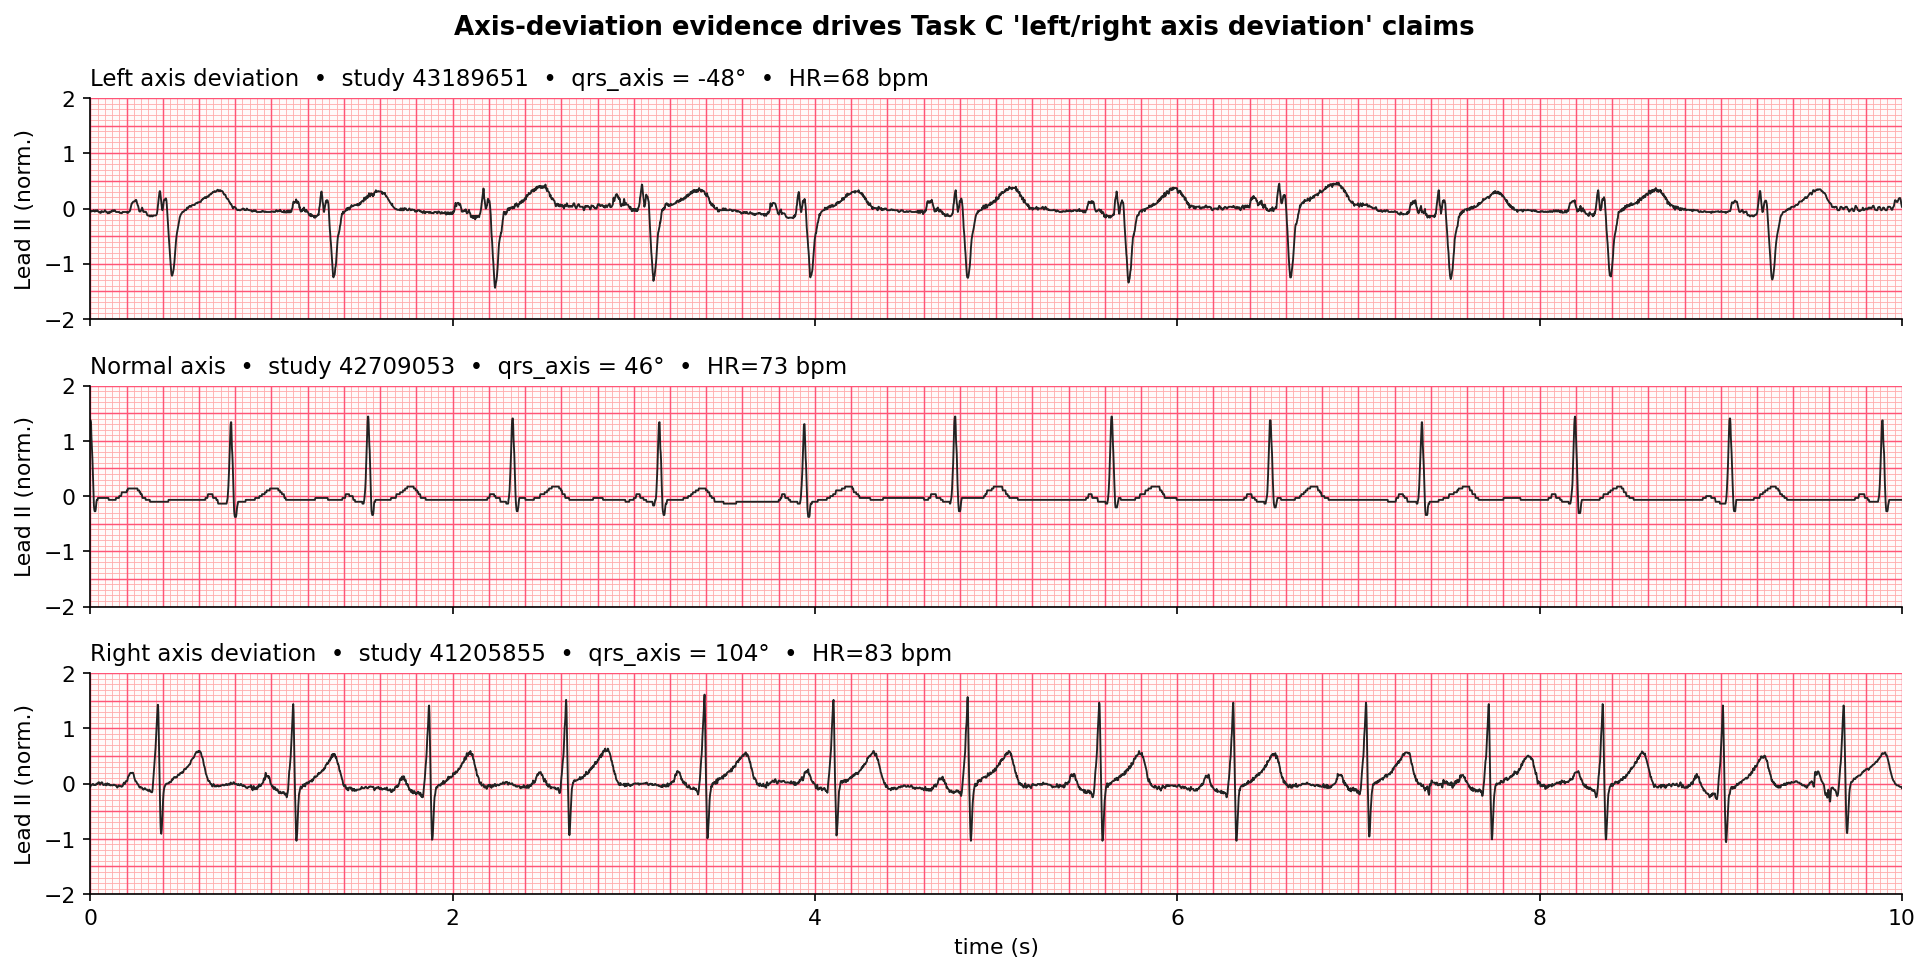
\includegraphics[width=\linewidth]{fig_axis_examples.png}
 \caption{Lead~II evidence for the three axis branches in Task~C. Left: $qrs\_axis=-48^\circ$ (\texttt{left axis deviation} SUPPORTED). Centre: $qrs\_axis=+46^\circ$ (\texttt{axis normal} SUPPORTED). Right: $qrs\_axis=+104^\circ$ (\texttt{right axis deviation} SUPPORTED).}
 \label{fig:axis_examples}
\end{figure}

\subsection*{Task A counts}

Task~A contains $5{,}597{,}755$ rows: each of the $799{,}706$ cleaned studies emits two positive rows (clean and scan-like image) and four canonical negatives (\texttt{TEXT\_SWAP}, \texttt{IMAGE\_SWAP}, \texttt{SIGNAL\_SWAP}, \texttt{PARTIAL\_MISMATCH}); the same-bucket \texttt{HARD\_NEGATIVE\_TEXT} is emitted for $799{,}519$ studies (the $187$ studies with invalid RR cannot be placed in a HR bucket and therefore have no eligible same-bucket sibling). Splits inherit from the patient split: train$=4{,}487{,}216$, val$=562{,}971$, test$=547{,}568$. Image type splits as clean$=4{,}798{,}049$ and scan-like$=799{,}706$ (the scan-like positive is emitted exactly once per study; standard negatives use clean images by construction). See Figure~\ref{fig:taskA_distribution} for the per-negative-type bar chart and \texttt{processed/taskA\_stats.json} for the persisted counts.

\subsection*{Task B counts}

Task~B contains $2{,}399{,}118$ rows = $799{,}706\times 3$ (one per query per study). Train$=1{,}923{,}159$, val$=241{,}281$, test$=234{,}678$. The fraction of studies with at least one positive bin is $53.92\%$ for \texttt{HIGH\_HEART\_RATE}, $33.17\%$ for \texttt{LOW\_HEART\_RATE}, and $49.83\%$ for \texttt{WIDE\_QRS}. Within the studies that have any positive bin, the fraction with \emph{mixed} labels (i.e., the label vector is not all-zero or all-one) is $84.8\%$ for \texttt{HIGH\_HEART\_RATE}, $87.8\%$ for \texttt{LOW\_HEART\_RATE}, and $99.4\%$ for \texttt{WIDE\_QRS}; this is the quantitative counterpart of Figure~\ref{fig:taskB_examples} and confirms that the local detector produces meaningful intra-study temporal variation rather than re-encoding the global \texttt{rr\_interval}.

\subsection*{Task C counts}

Task~C contains $4{,}726{,}480$ rows: $2{,}398{,}931$ \texttt{SUPPORTED}, $2{,}327{,}175$ \texttt{CONTRADICTED}, and $374$ \texttt{UNCERTAIN}. The eight claims and their row counts are summarised in Table~\ref{tab:taskC_claim_counts}. Splits: train$=3{,}789{,}152$, val$=475{,}014$, test$=462{,}314$.

\begin{table}[!ht]
\centering
\caption{Task~C per-claim row counts.}
\label{tab:taskC_claim_counts}
\renewcommand{\arraystretch}{1.2}
\begin{tabular}{l r}
\toprule
Claim & Rows \\
\midrule
\texttt{tachycardia present}    & 799{,}706 \\
\texttt{bradycardia present}    & 799{,}706 \\
\texttt{wide qrs complex}       & 799{,}706 \\
\texttt{normal qrs duration}    & 799{,}706 \\
\texttt{normal heart rate}      & 574{,}308 \\
\texttt{axis normal}            & 646{,}064 \\
\texttt{left axis deviation}    & 153{,}642 \\
\texttt{right axis deviation}   & 153{,}642 \\
\bottomrule
\end{tabular}
\end{table}

\subsection*{Differences from MEETI on shared statistics}

Where both releases describe the same underlying MIMIC-IV-ECG measurement, our central-tendency numbers are very close to those reported in MEETI~\cite{zhang2024meeti}: median HR $74.07$~bpm (MEETI: $74.50$), median QRS duration $94$~ms (MEETI: $91$ for FeatureDB-extracted per-beat duration), median QT $396$~ms (MEETI: $371$), median QRS axis $14^\circ$ (MEETI does not report axis separately). The slight differences are expected because MEETI computes per-beat features with FeatureDB whereas Tri-Modal-ECG inherits MIMIC's record-level machine measurements, but the agreement on the medians supports the validity of both extractions. The major release-level differences (image coverage, scan-like stream, deterministic benchmarks, patient-level split) are shown in Figure~\ref{fig:feature_matrix} and discussed in the Background~\&~Summary.

\section*{Usage Notes}

\textbf{Authoritative entry point.} The single source of truth for the dataset is \bpath{processed/index/index_clean_with_measurements.parquet}. Every benchmark task is generated from this index, and every per-study QC JSON is keyed by the same \texttt{study\_id}. Users who only need a tabular interface to the cleaned dataset can ignore the JSONL files entirely.

\textbf{Splits.} Splits in our parquet and JSONL files are patient-level. \emph{Do not} re-shuffle records at the row level; doing so silently introduces patient leakage, which is a well-documented methodological pitfall in ECG benchmarking on PTB-XL-style corpora \cite{strodthoff2021deep, ribeiro2020automatic}.

\textbf{Image modality choice.} Models that ingest only the clean PNG will be exposed to a more uniform pixel distribution than they will see in a deployed setting. We strongly recommend training (or at least evaluating) on the scan-like JPG; the deterministic seed makes this reproducible and safe to combine with the patient-level split.

\textbf{Sentinel codes.} The structured-measurement columns inherit MIMIC's sentinel codes (\texttt{29999, 32767, 65535, $-32768$, $0$}) for missing values. Apply the physiological-plausibility filters described in Section ``Distribution of structured measurements'' before computing summary statistics. The benchmark-task generators apply task-specific handling: Task~A uses HR buckets that map invalid RR to ``no bucket''; Task~C emits an UNCERTAIN row when the relevant measurement is missing.

\textbf{Local detection vs.\ global stamps.} Task~B's labels are produced by NeuroKit2 \cite{makowski2021neurokit2} R-peak detection \cite{pan1985realtime} and wavelet QRS delineation \cite{martinez2004wavelet}; the global RR-based fallback only fires when local detection raises an exception. Users who want the all-bins-equal global rule for ablations can recompute it from the structured measurements; users who want stricter local detection can replace NeuroKit2 with their preferred pipeline by editing \texttt{scripts/task\_B.py}.

\textbf{No LLM in the loop.} All benchmark labels are deterministic functions of the structured measurements and Lead~II signal. There is no GPT-4o or similar LLM call in the data pipeline; this is the main reason the benchmark tasks are reproducible across rebuilds and across hardware.

\textbf{Limitations.} (1)~Task~B's R-peak detector inherits the failure modes of Pan-Tompkins on extremely noisy signals; the QC pipeline removes flatline records but cannot remove every noisy beat. The global fallback is conservative on \texttt{WIDE\_QRS} (always-zero), which slightly underestimates wide-QRS prevalence in noisy studies. The start-of-signal artefact filter described in Section ``Task~B'' handles the most common Pan-Tompkins failure mode (a spurious leading R-peak inside the first $\sim$300~ms) but is intentionally narrow: it only drops a leading peak when both the relative-RR ratio test and the absolute $171$~bpm test fire. Real first beats with short RR intervals (e.g., a tachycardic burst at the very start) are preserved. (2)~Task~C uses MIMIC's record-level machine measurements rather than per-beat measurements; deeper investigations of beat-level variability (e.g., heart-rate variability, dynamic QT prolongation) are better served by the per-beat FeatureDB extraction shipped with MEETI \cite{zhang2024meeti}. (3)~Both release-time runtime numbers and intermediate failure counts are persisted only for the scan-like generation pass; runtimes for clean rendering, QC, and the three task generators are printed to the console but not durably logged. (4)~The released audit-md notes minor schema drift between this paper's JSONL keys (\texttt{labels}, \texttt{claim}, \texttt{label}) and an earlier rule-book ($y\_bins$, $claim\_tag$, $y\_support$); we have prioritised the schemas as actually generated, and downstream tooling should follow Tables~\ref{tab:taskA_schema}--\ref{tab:taskC_schema}.

\section*{Resource Availability}

The full code base used to construct Tri-Modal-ECG (signal extraction, image rendering, scan-like augmentation, QC, regeneration, splitting, measurement enrichment, and the three task generators) is shipped under \texttt{scripts/}. The on-disk artefacts described in Section ``Data Records'' are produced from the public MIMIC-IV-ECG dataset under the PhysioNet-credentialed-access licence \cite{gow2023mimic, johnson2020mimic}; users must agree to that licence and download the upstream data themselves before running our pipeline. The Python environment used for this work is captured in \texttt{ecg\_env/} (CPython, NumPy~\cite{harris2020array}, Matplotlib~\cite{hunter2007matplotlib}, OpenCV~\cite{bradski2000opencv}, WFDB~\cite{xiao2018physionet}, NeuroKit2~\cite{makowski2021neurokit2}, pandas with PyArrow~\cite{vaynberg2020apache}). The full reproducible pipeline order, persisted runtime evidence, and a verification checklist are included as appendices in the accompanying technical report (\bpath{TRI_MODAL_ECG_UNDERSTANDING_SYSTEM_REPORT.md}).

\section*{Acknowledgments}

This work uses the MIMIC-IV-ECG release~\cite{gow2023mimic, johnson2020mimic} and was inspired by the MEETI extension~\cite{zhang2024meeti}, whose four-component vision (signal + image + features + interpretation) motivated the design of Tri-Modal-ECG.

\section*{Author Contributions}

N.C., B.R.R. and A.M. jointly designed the pipeline, implemented the codebase, generated and audited the dataset, conducted the technical validation, and prepared the manuscript. All authors reviewed and approved the final version.

\section*{Declaration of Interests}

The authors declare no competing interests.

\newpage

\bibliography{references}

\end{document}
